\chapter{Evaluation}\label{chap:evaluation}
In this chapter, we present our evaluation criteria and the findings which we got from them.
We evaluate the four models with a three-pronged strategy, targeting the following characteristics:

\begin{enumerate}
    \item\textbf{Accuracy} - the share of correct next-activity predictions
    \item\textbf{Training time} - the amount of time required for training
    \item\textbf{Stability} - the change in prediction accuracy with progress
\end{enumerate}

The first two criteria target the general usability of each model.
We measure accuracy because it is a good indicator of how often the model predicts the right class, and permits comparisons to other works.
Different from typical machine learning evaluations, we do not measure recall, because it is not typically measured by works in Predictive Process Monitoring.
Training time is of interest because a real-world application should use as little computing resources as possible.
The stability criterion permits making a judgment about the behavior of accuracy over time. The works of Francescomarino et al.~\cite{francescomarino2015} and Klinkmüller et al.~\cite{klinkmuller2018reliablemonitoring} inspired this measure. It provides an understanding of how the prediction accuracy of a model changes as the trace grows longer. This can facilitate building trust in the model, as indicated in the introduction of the thesis~\cite{klinkmuller2018reliablemonitoring, boehmer2018probability}.
During the evaluation, results for BPIC logs and the HelpDesk dataset should not be compared too closely, as the BPIC logs are a lot more resourceful in terms of data attributes.

We discuss the acurracy of the models in \autoref{sec:eval:accuracy}, followed by the discussion of the required training time in \autoref{sec:eval:training-time}. We go on to discuss stability in \autoref{sec:eval:stability}, and conclude the chapter in \autoref{sec:eval:discussion}.

\section{Accuracy}\label{sec:eval:accuracy}
The accuracy on unseen data is a good indicator for how well a model predicts.
It is the share of correct predictions that match their target labels among the number of total predictions:

$$\frac{n_{correct}}{n_{total}} $$

In the following paragraphs, we present the maximum accuracies obtained on the validation set of each log.
For each log, we show a plot of the different model accuracies, grouped by batching strategy.
The presentation of the logs is ordered by process complexity, similar to \autoref{tab:dataset-characteristics}.
We end the section with a verdict of the observations.\\

% individual strategy
\paragraph{Accuracy on HelpDesk}
\autoref{fig:max-accuracies-helpdesk} displays the different accuracies on the validation set from the HelpDesk log.
With the individual, grouping and padding strategies, the SCH, SP2 and PFS models score above $0.80$.
As expected, the windowing strategy impacts accuracy significantly, with all models seeing large degradations.
The SP2 model is impacted the least by the windowing strategy, presumably because its SP2 features capture the history that is cut away.
While the SCH, SP2 and PFS models do not show strong reactions to changes in the first three batching strategies, the accuracies by the EVM model fluctuate immensely.
On the individual strategy, it exhibits $0.724$.
On the grouping and padding strategies, the EVM model delivers $0.316$ and $0.3$.

\begin{figure}[!htb]
    \centering
    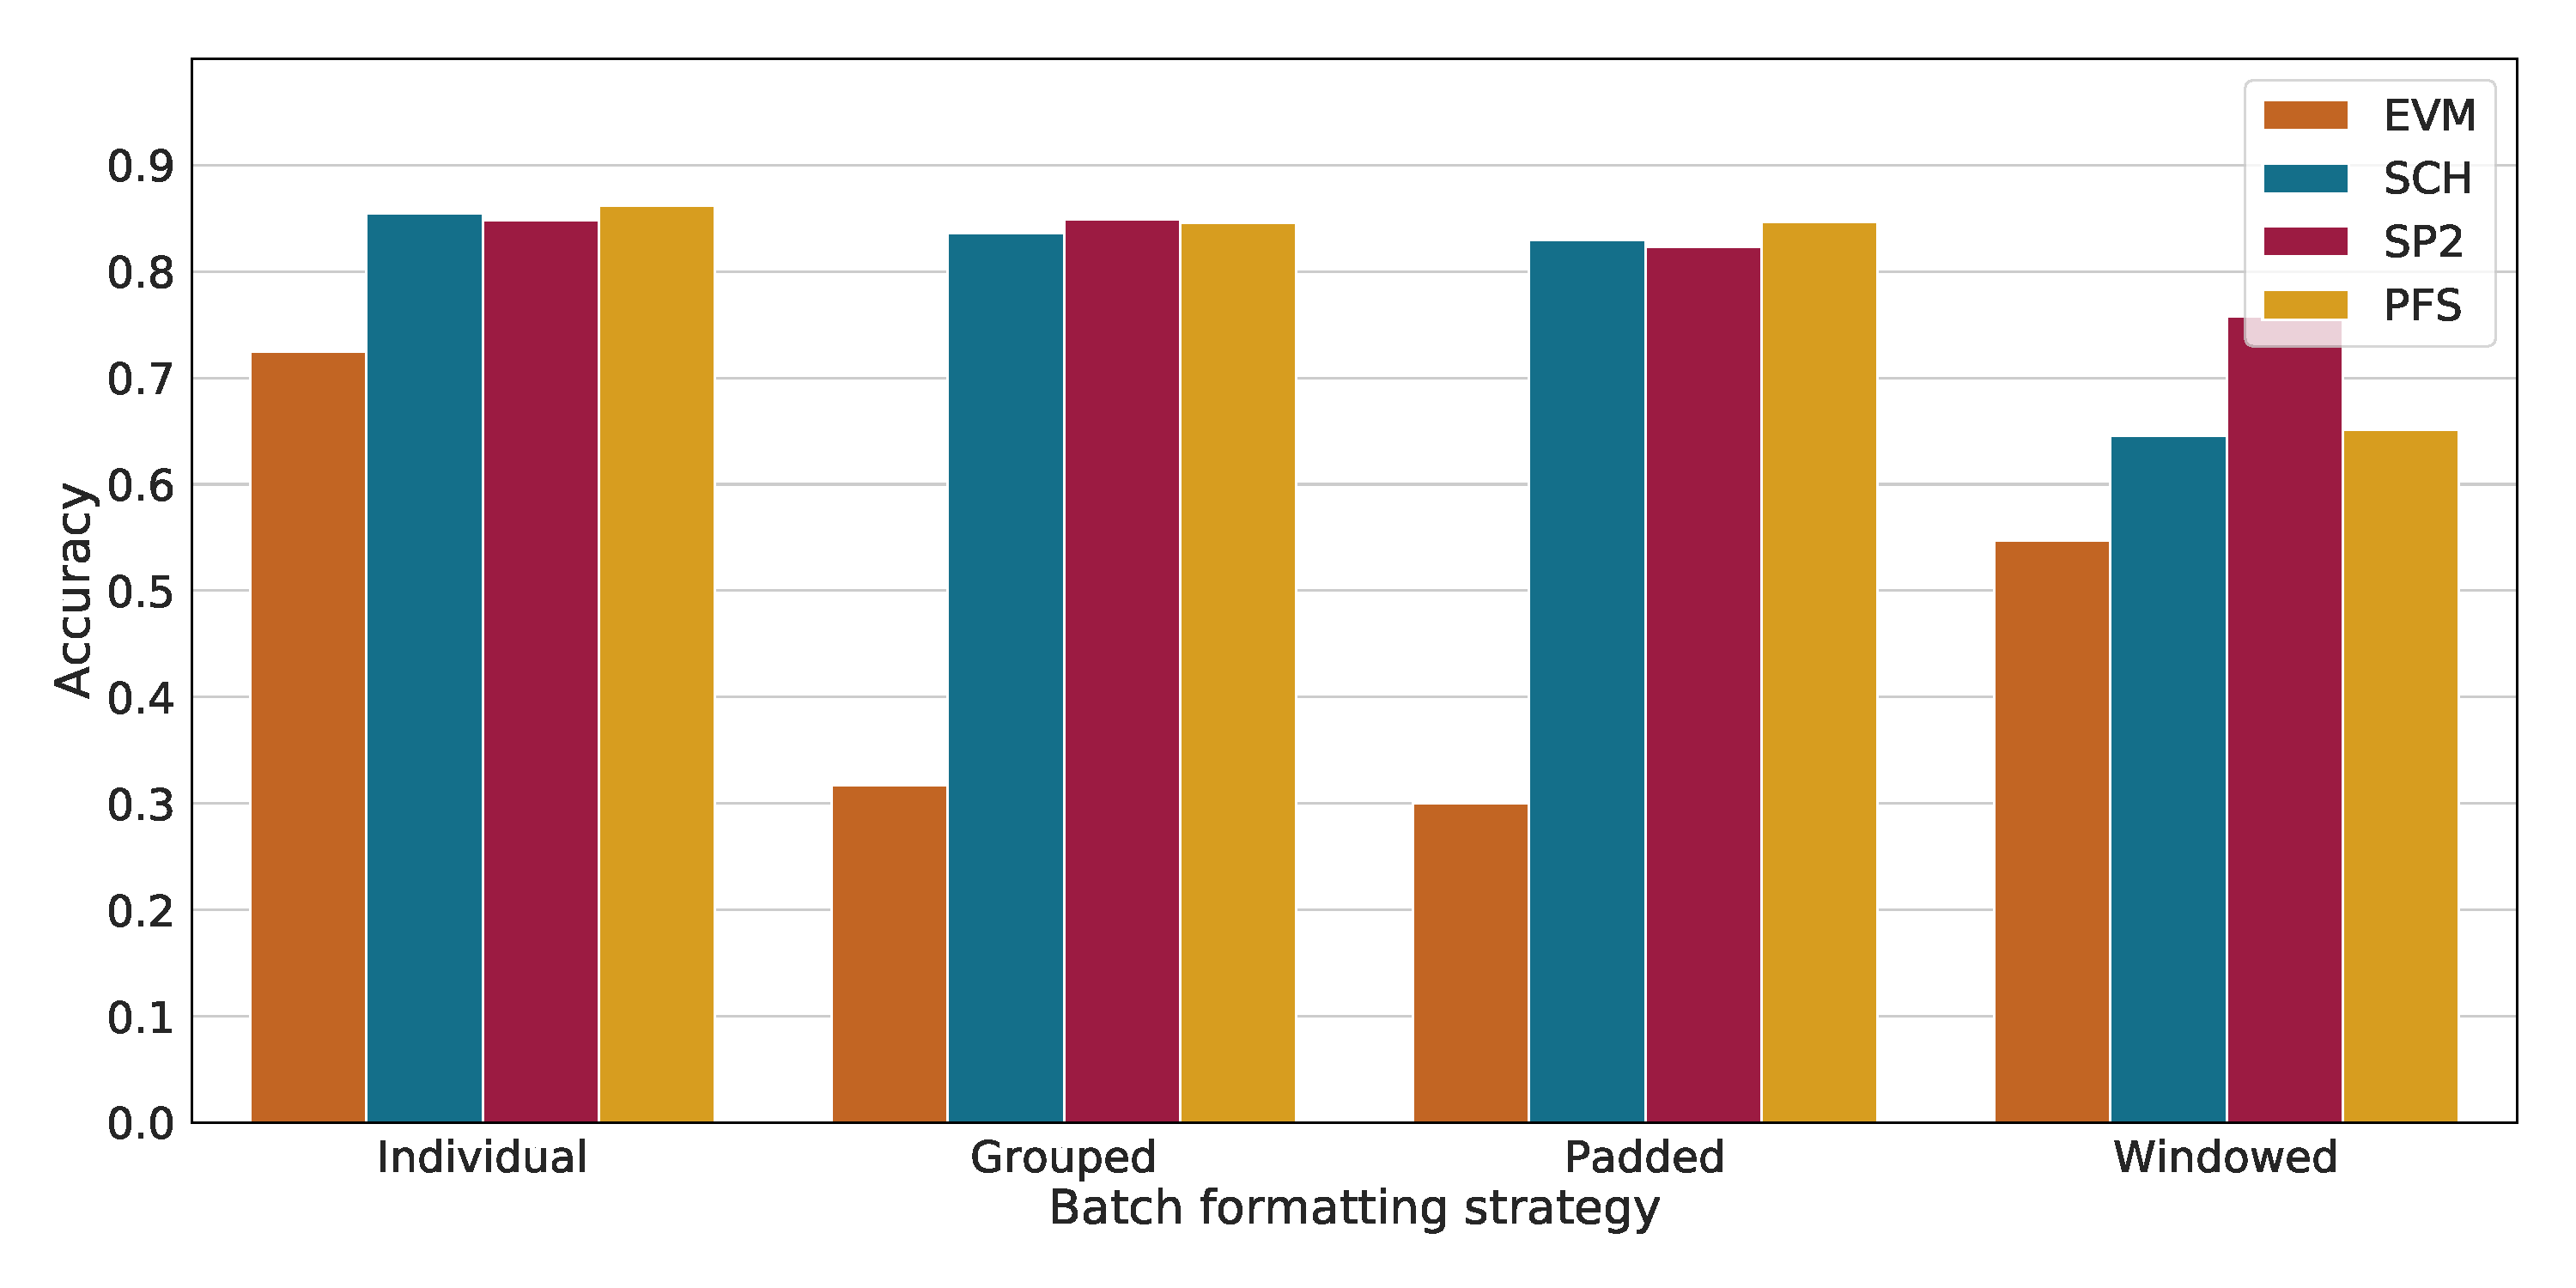
\includegraphics[width=\textwidth]{gfx/helpdesk/accuracies.pdf}
    \caption{Best accuracies on the validation set of HelpDesk}
    \label{fig:max-accuracies-helpdesk}
\end{figure}

\paragraph{Accuracy on BPIC12}
BPIC12 is a small step up in process complexity, and the accuracy measurements are visualized in \autoref{fig:max-accuracies-bpic2012}.
Again, the EVM, SCH, and SP2 models exhibit very similar accuracies for the three batching strategies that supply the complete process history.
With the individual and padding strategies, all three of them reach over $0.840$.
In the case of the grouping strategy, the three accuracies are between $0.750$ and $0.765$.
The windowing strategy leads to more significant differences between the SCH, SP2 and PFS models.
Here, the SP2 models outperform all other models.
The worst performance is again shown by the EVM model on all four strategies, while its accuracies with the individual and grouping strategies are very similar.

\begin{figure}[!htb]
    \centering
    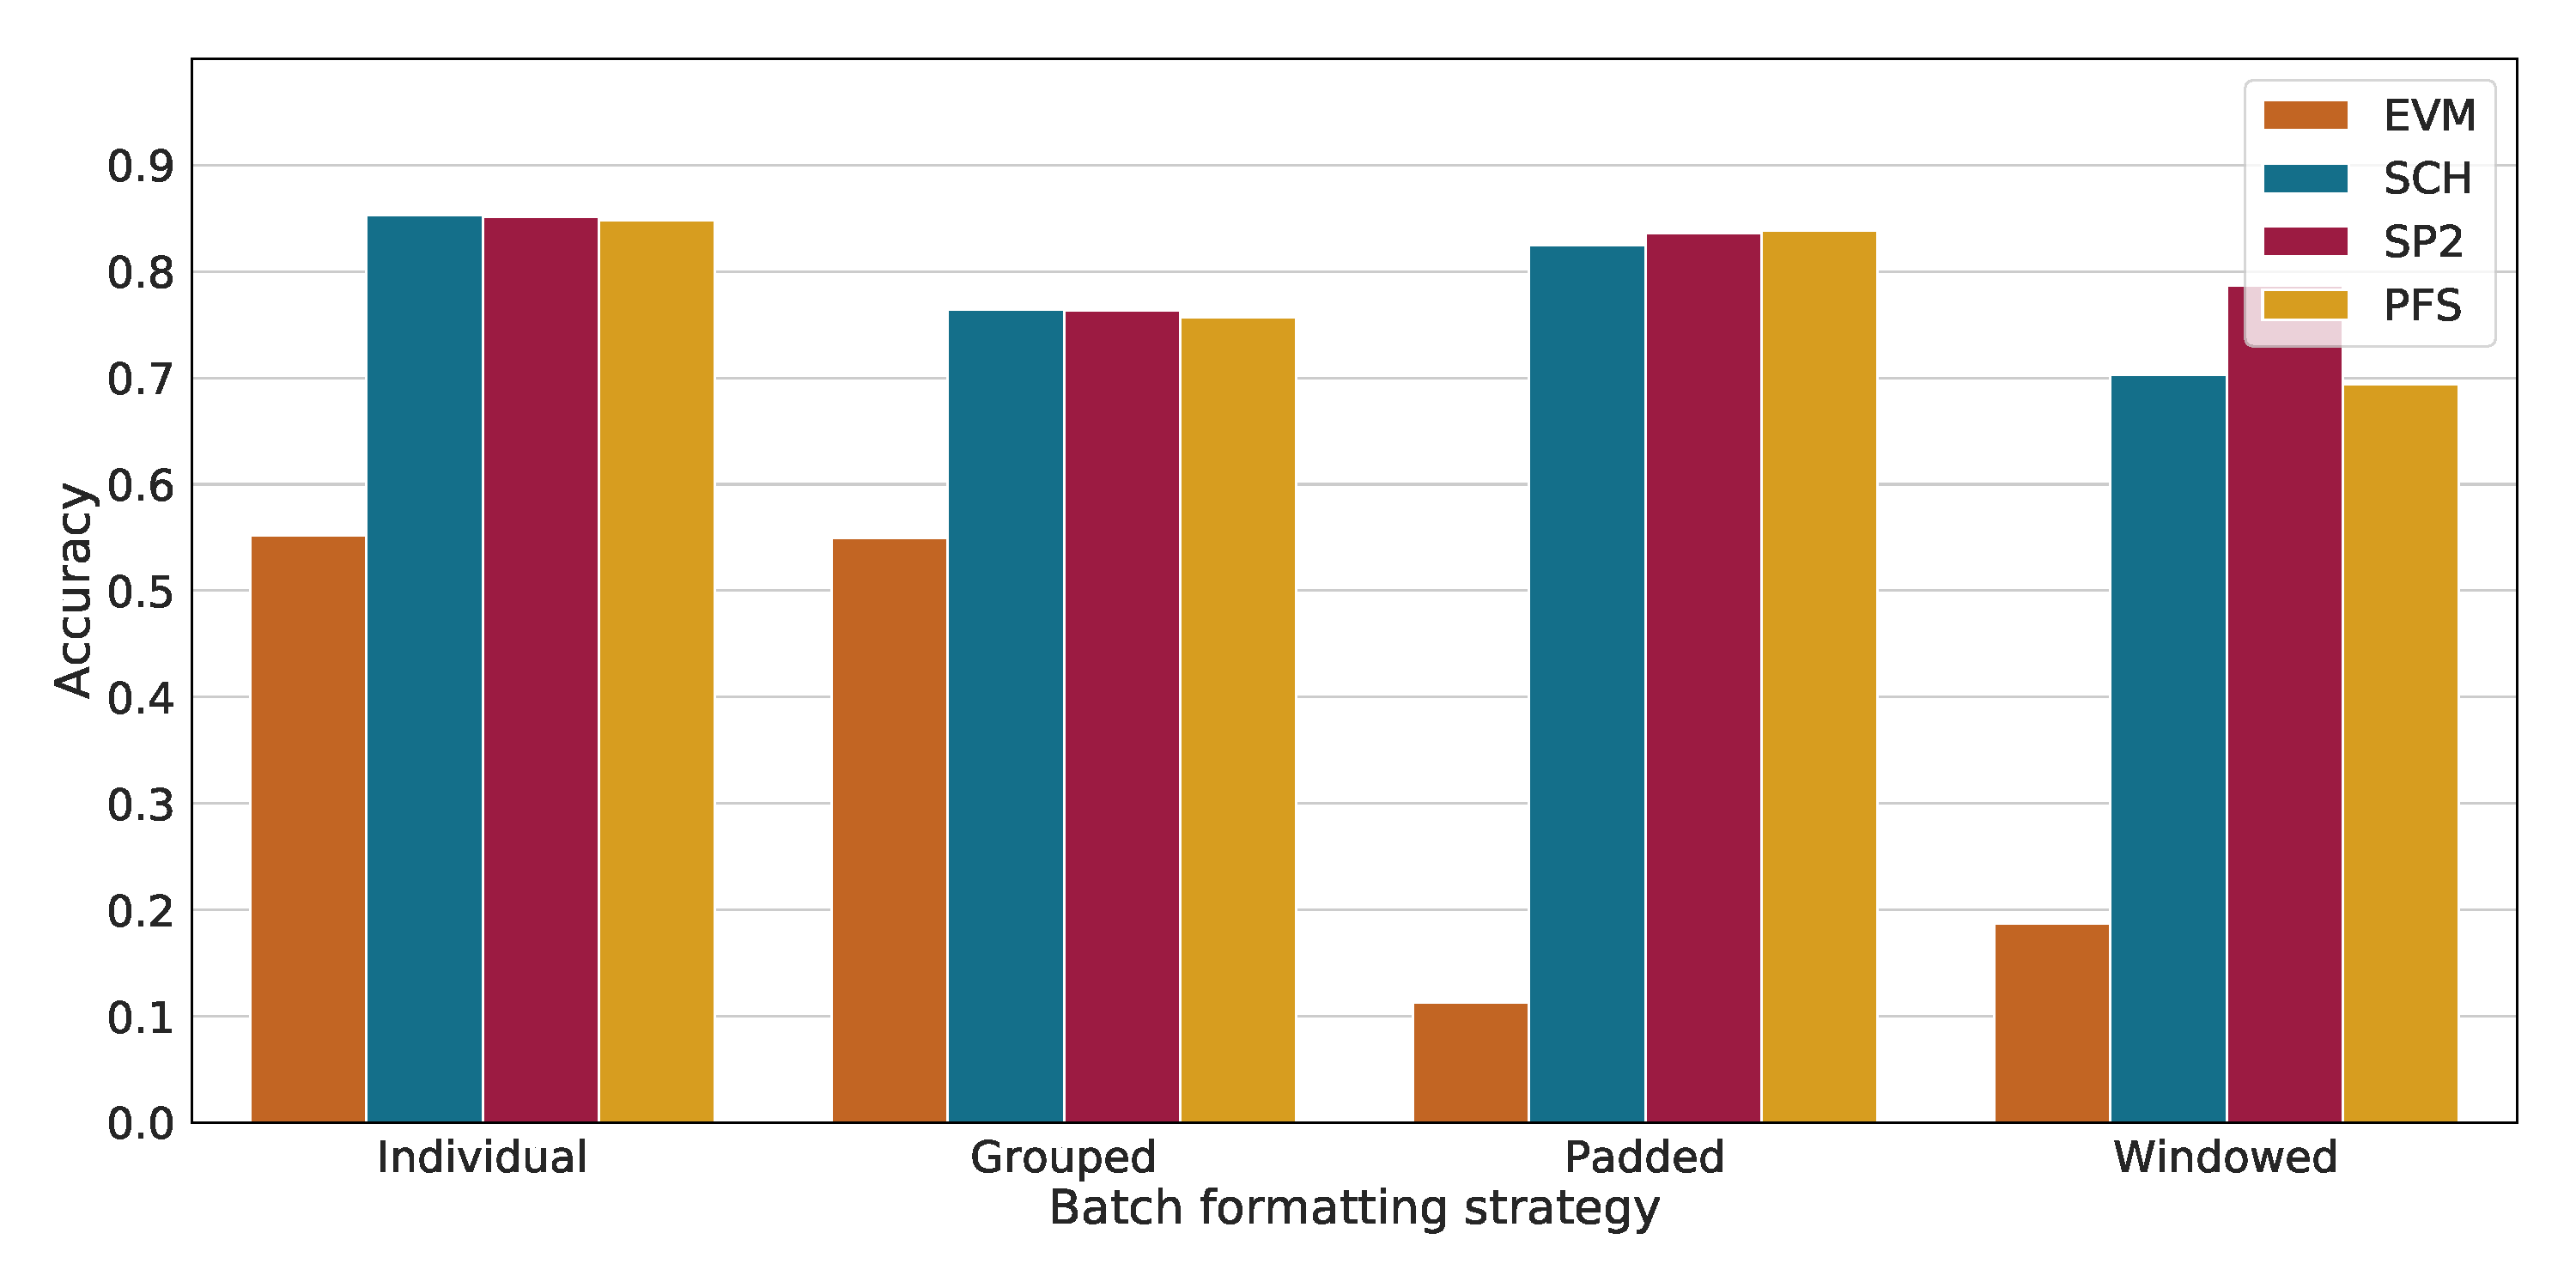
\includegraphics[width=\textwidth]{gfx/bpic2012/accuracies.pdf}
    \caption{Best accuracies on the validation set of BPIC12}
    \label{fig:max-accuracies-bpic2012}
\end{figure}

\paragraph{Accuracy on BPIC15}
The accuracies obtained on the validation sets of the BPIC15 logs are visualized in \autoref{fig:max-accuracies-bpic2015-1} to \autoref{fig:max-accuracies-bpic2015-5}.
The results are very similar, so we summarize four common themes that emerge in the plots:

First, the accuracies of the SCH, SP2 and PFS models are very similar across the individual, grouping and padding strategies.

Second, the SCH model always gives the highest accuracy of the four models with the individual strategy.

Third, the SP2 model gives the highest accuracies on all other strategies.
Also, its accuracies on the windowing strategy are the highest by far.
%We presume that this is caused by the SP-2 features which encode some of the history that was cut away during windowing.

Fourth, the EVM model accuracies are unusable. While still above $0.1$ on the individual and grouping strategies, the model completely breaks down on the others.

\begin{figure}
    \centering
    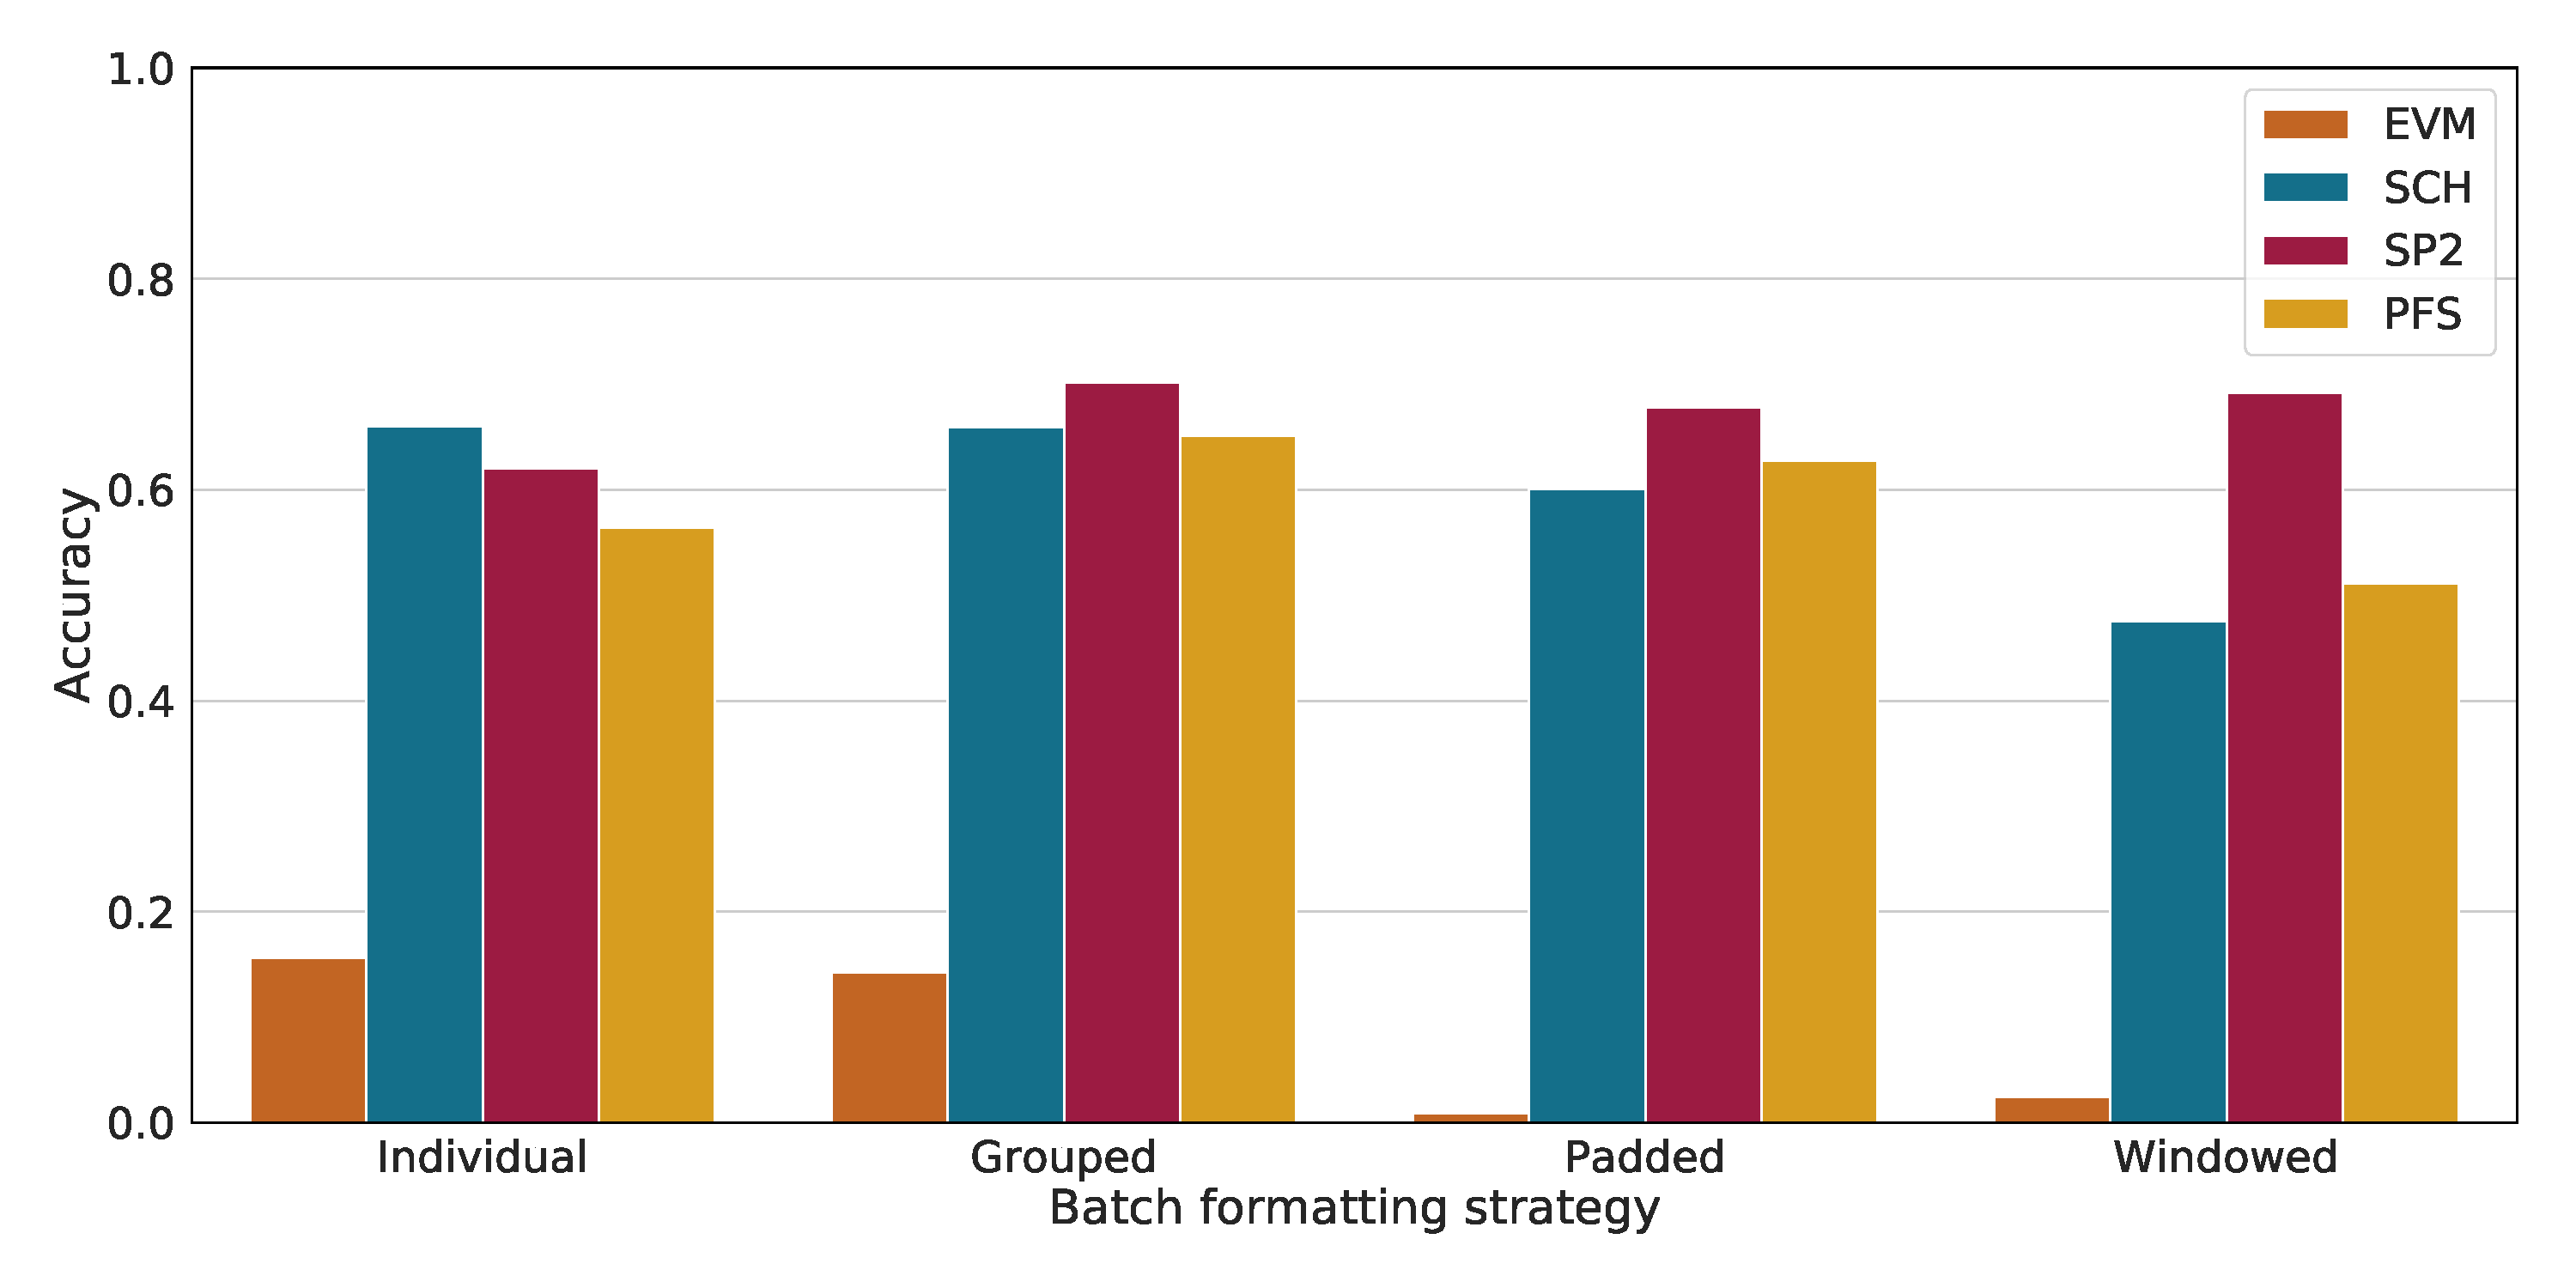
\includegraphics[width=\textwidth]{gfx/bpic2015_1/accuracies.pdf}
    \caption{Best accuracies on the validation set of BPIC15-1}
    \label{fig:max-accuracies-bpic2015-1}
\end{figure}
\begin{figure}
    \centering
    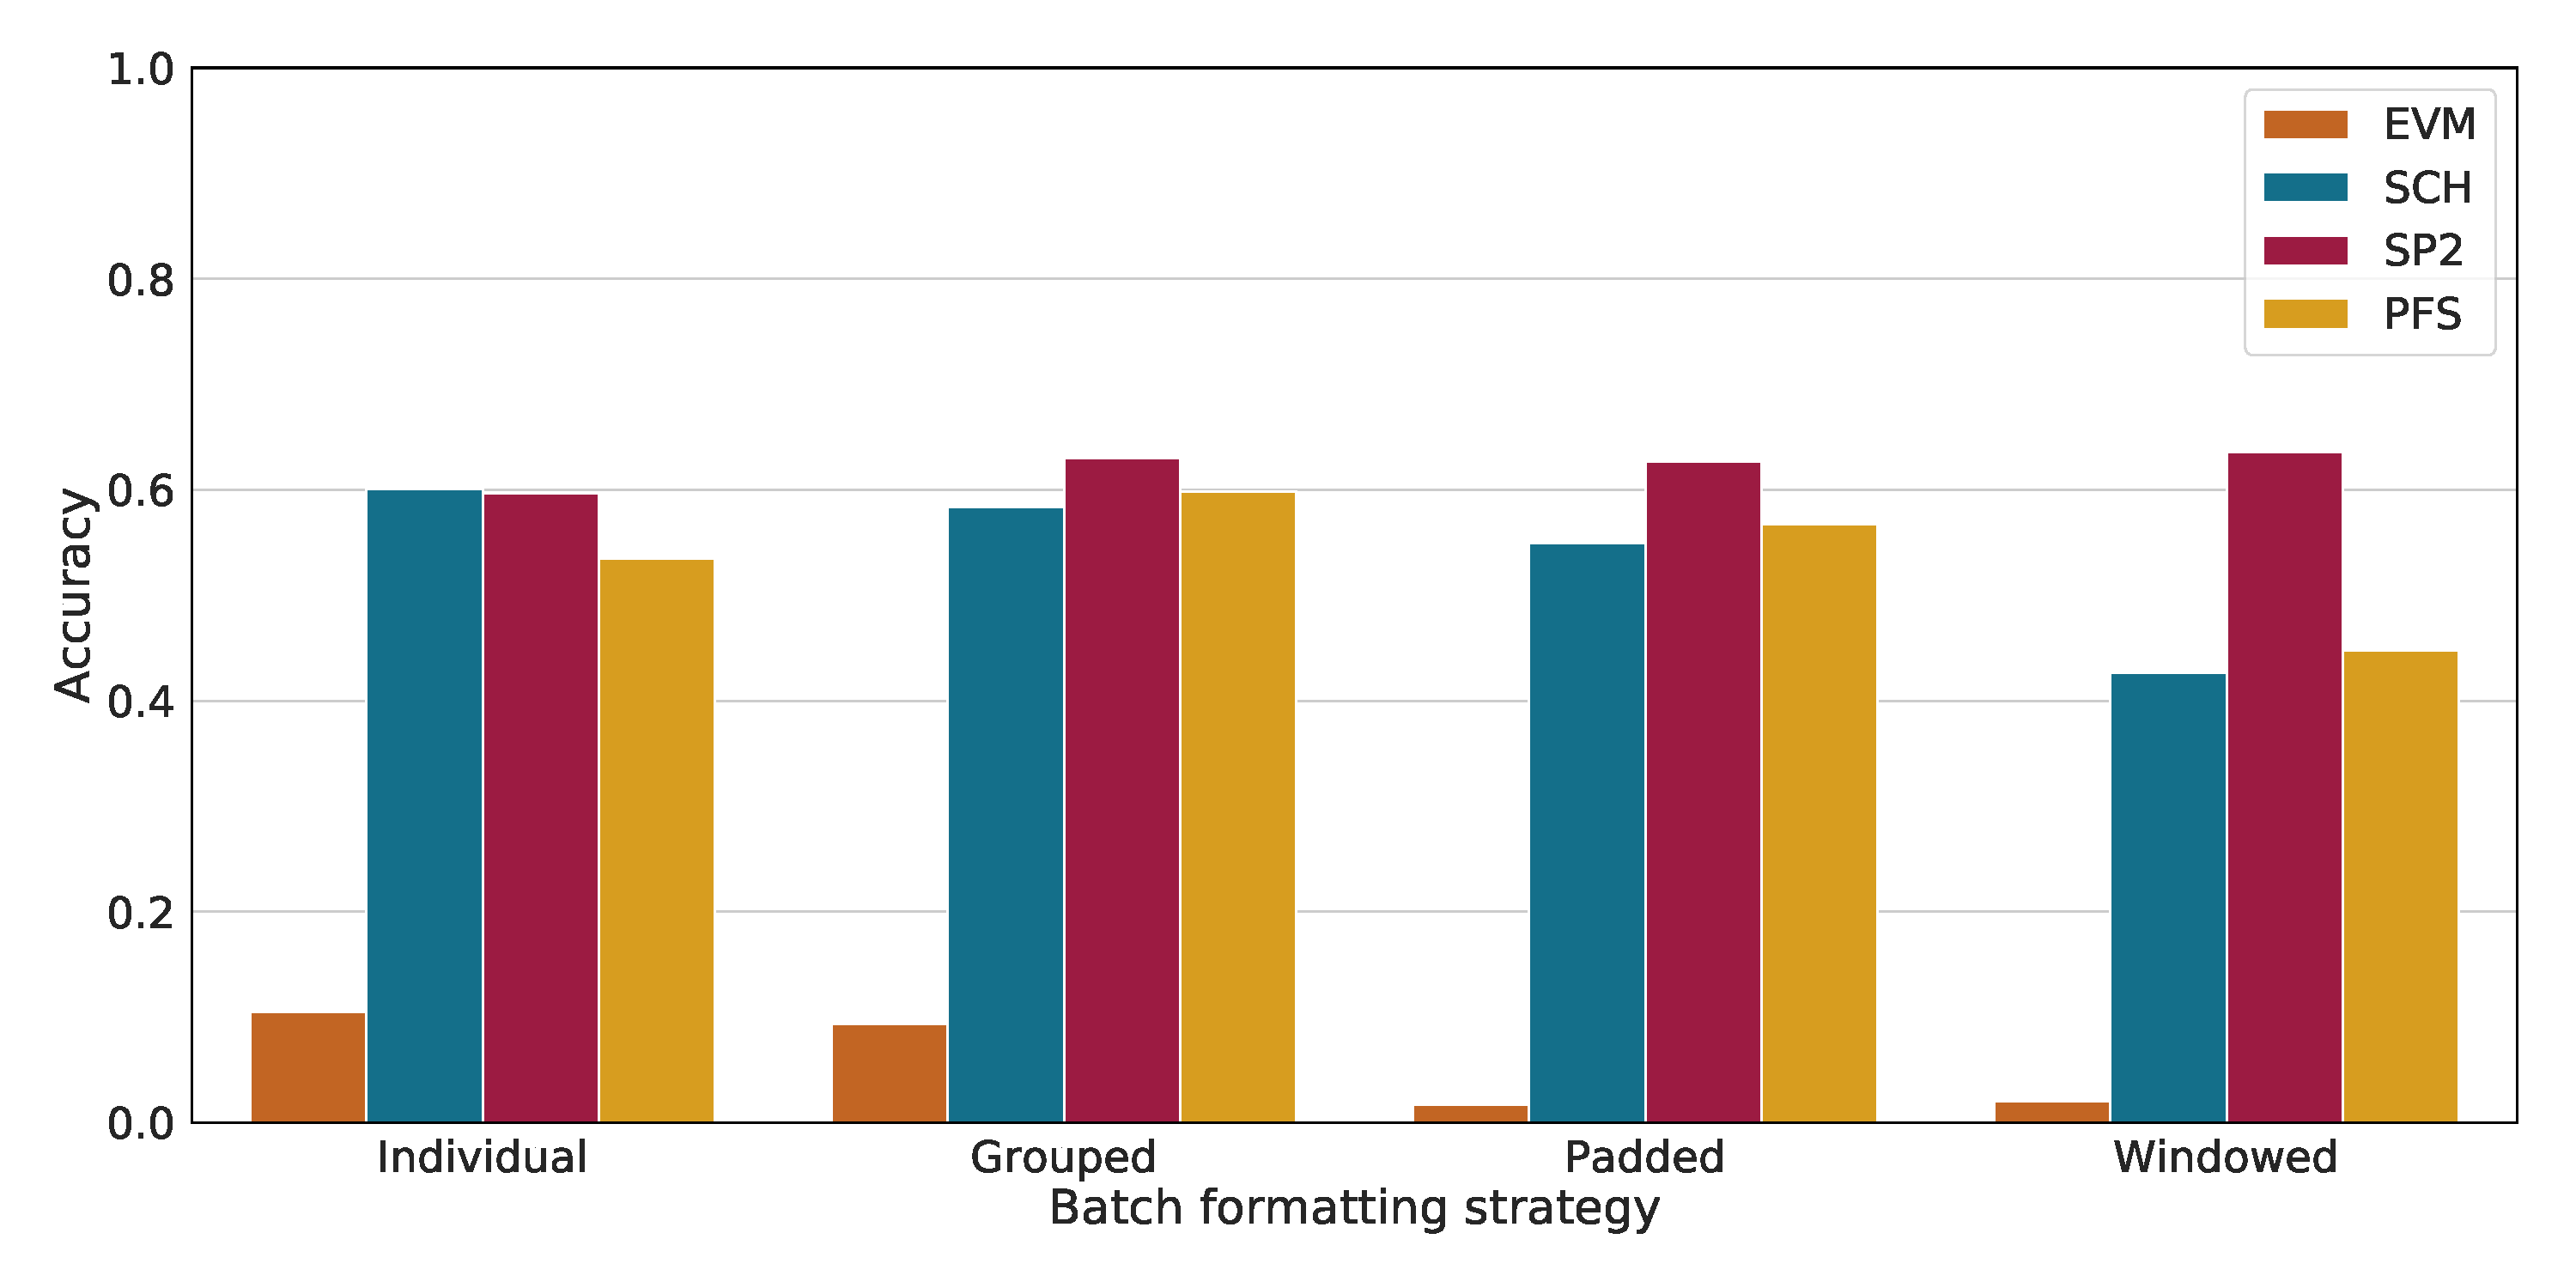
\includegraphics[width=\textwidth]{gfx/bpic2015_2/accuracies.pdf}
    \caption{Best accuracies on the validation set of BPIC15-2}
    \label{fig:max-accuracies-bpic2015-2}
\end{figure}
\begin{figure}
    \centering
    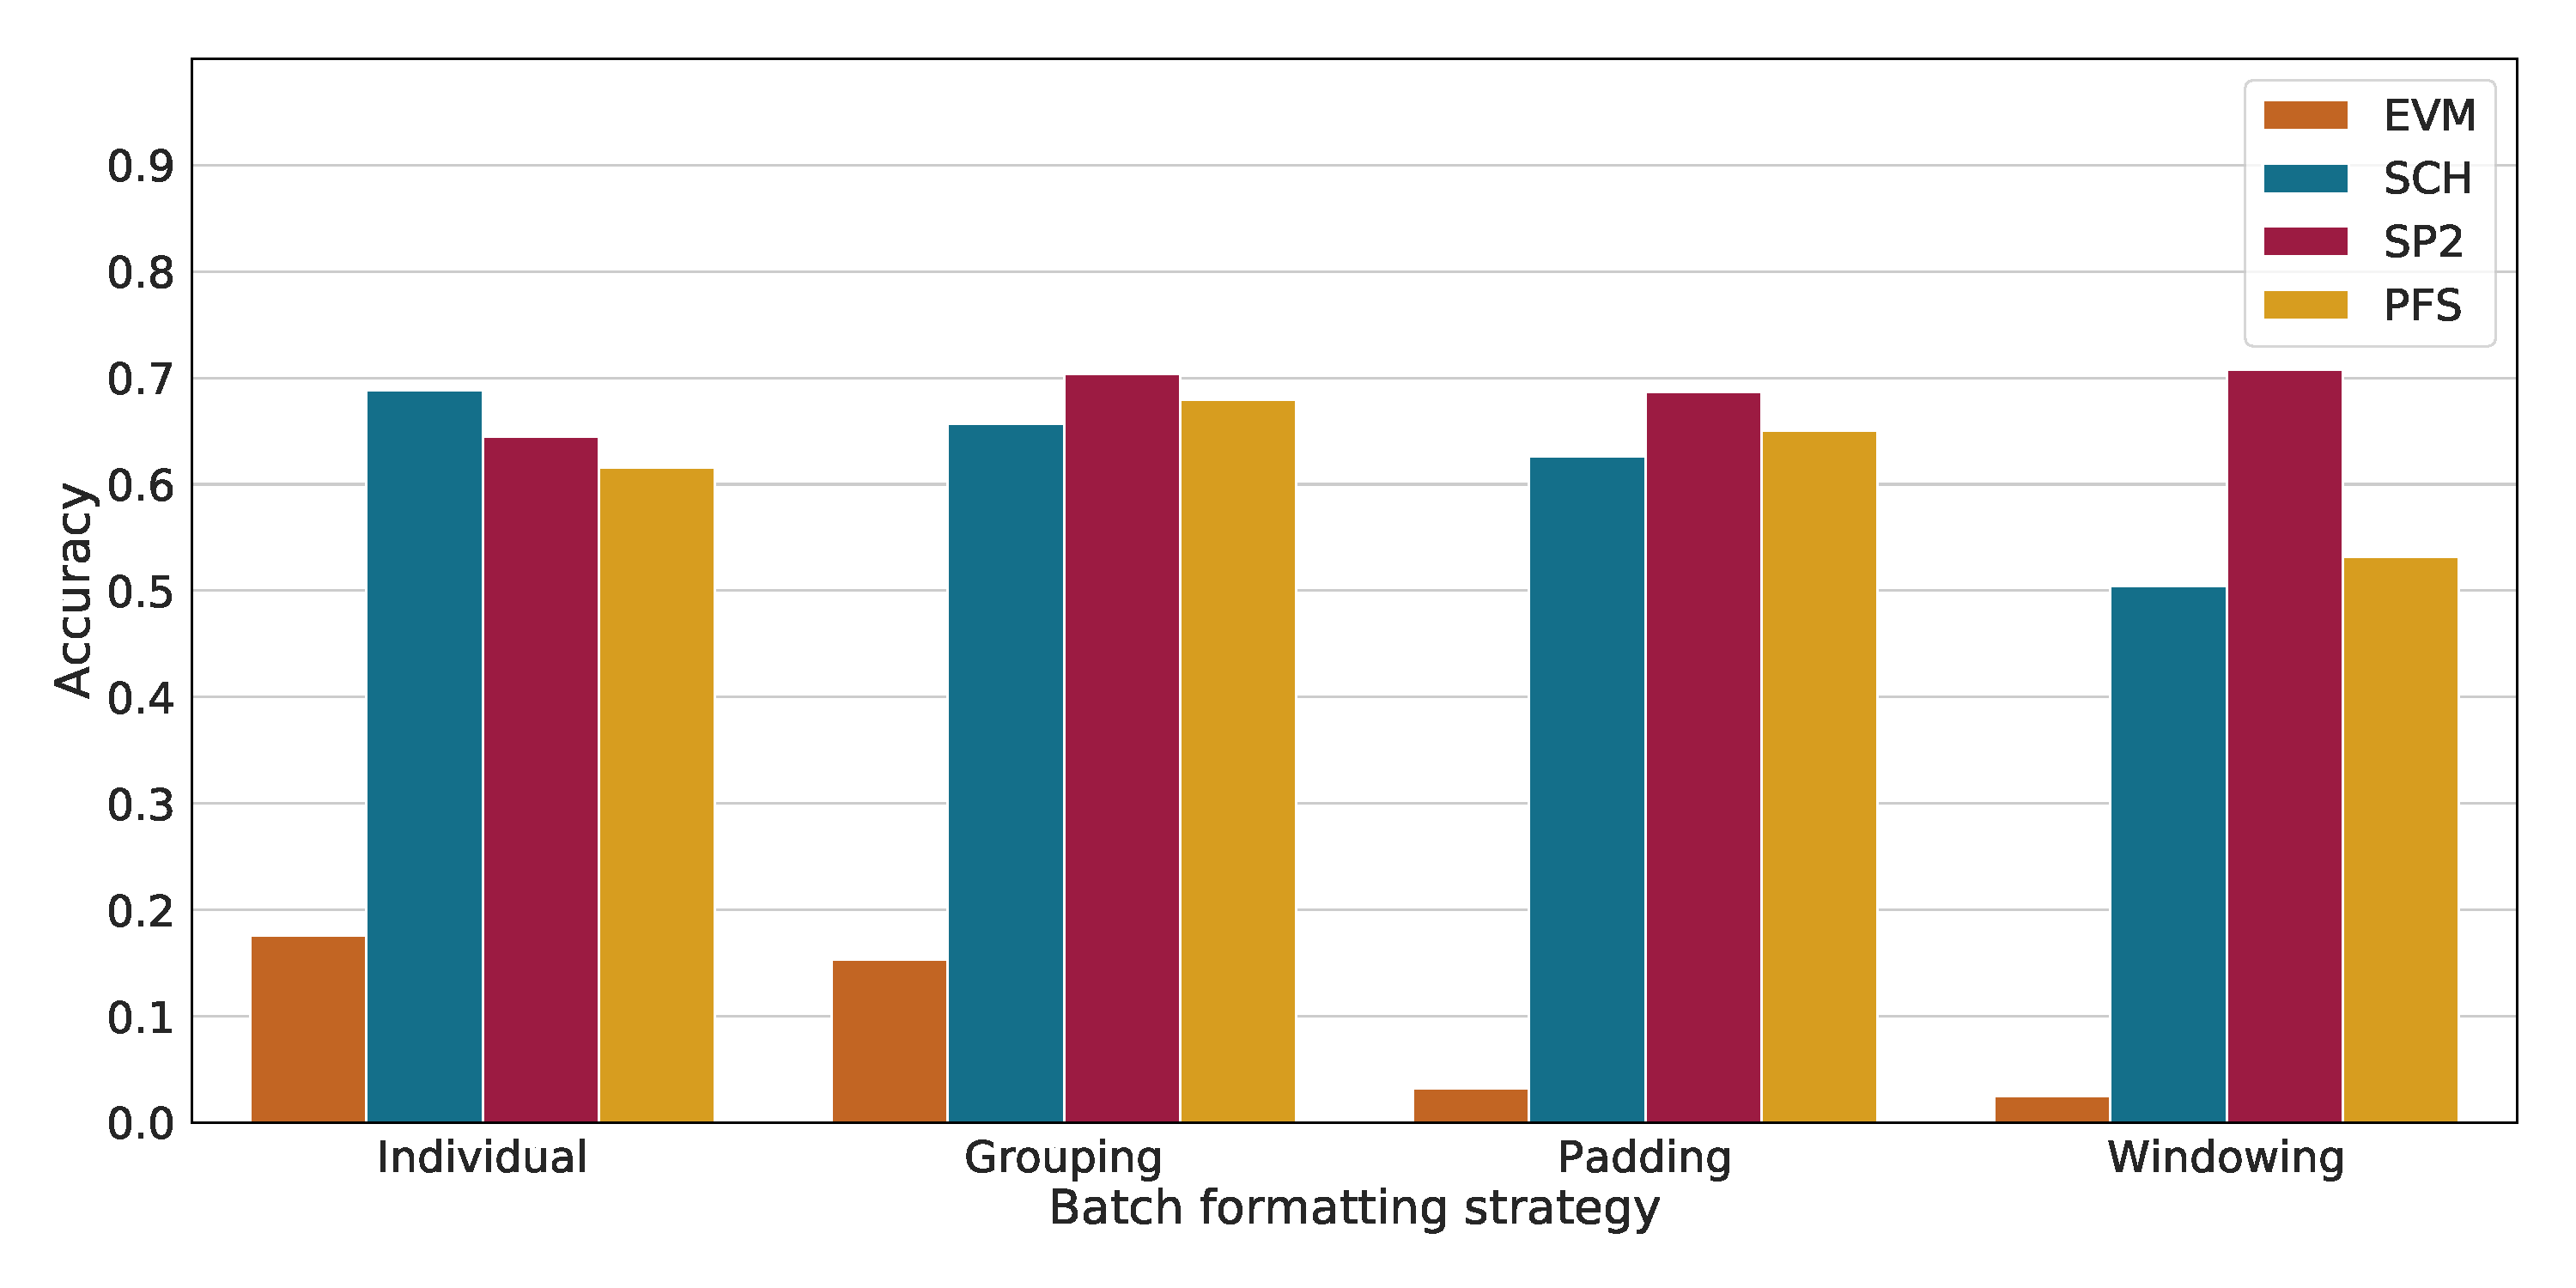
\includegraphics[width=\textwidth]{gfx/bpic2015_3/accuracies.pdf}
    \caption{Best accuracies on the validation set of BPIC15-3}
    \label{fig:max-accuracies-bpic2015-3}
\end{figure}
\begin{figure}
    \centering
    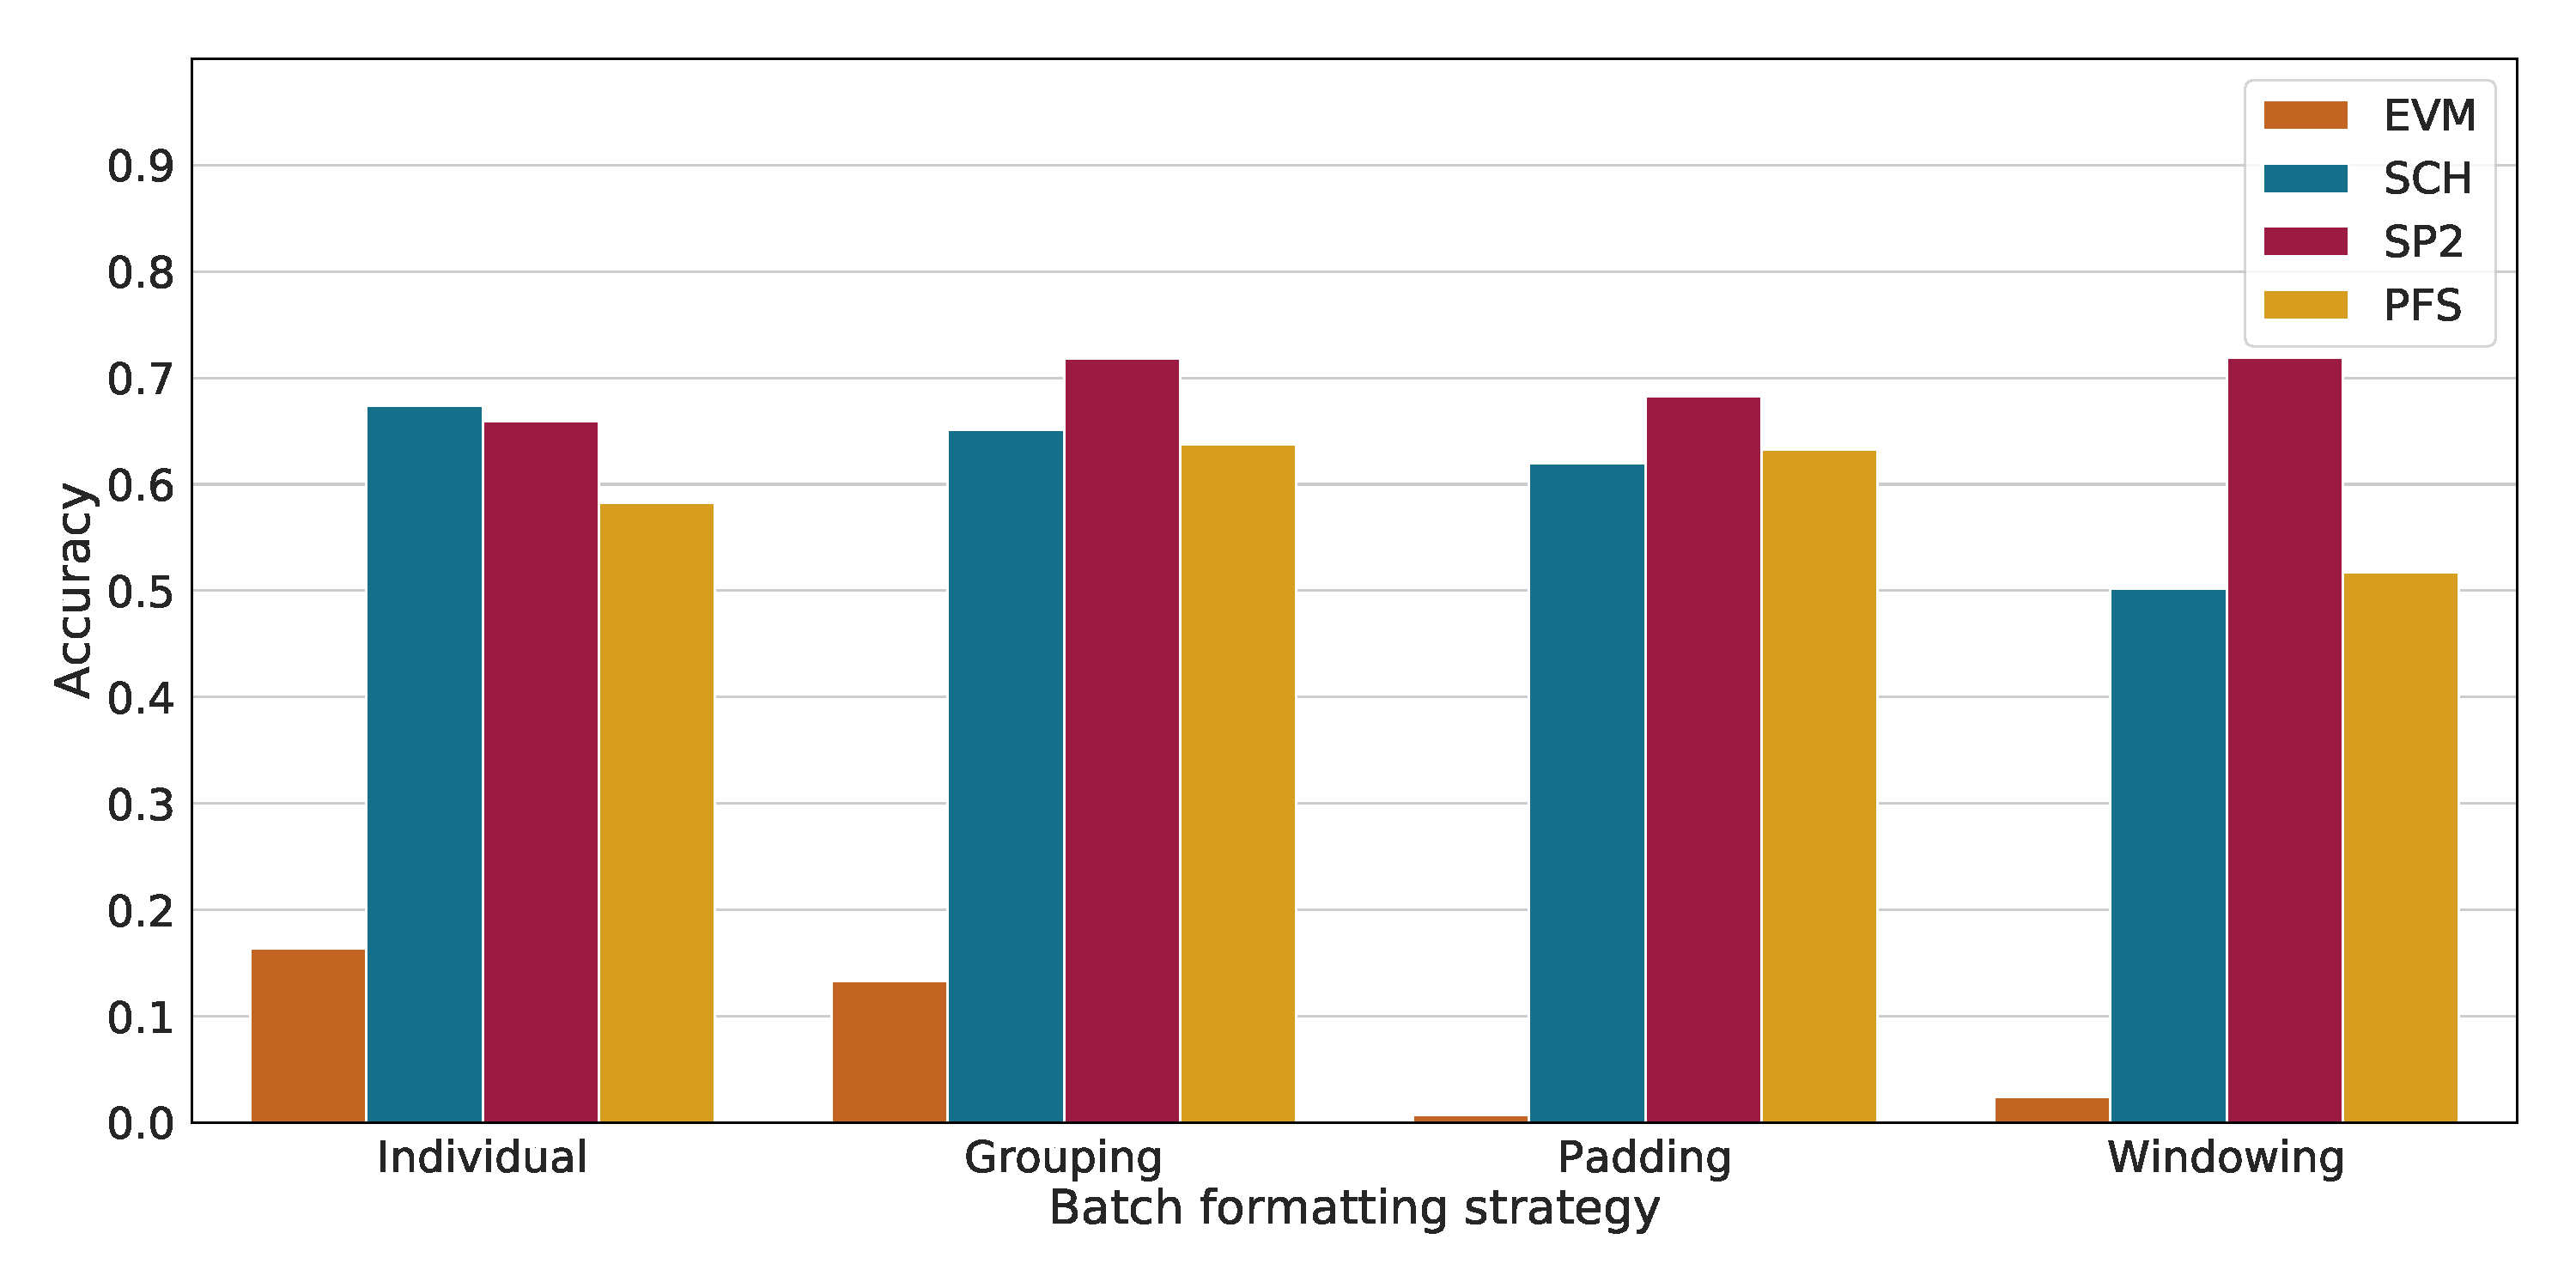
\includegraphics[width=\textwidth]{gfx/bpic2015_4/accuracies.pdf}
    \caption{Best accuracies on the validation set of BPIC15-4}
    \label{fig:max-accuracies-bpic2015-4}
\end{figure}
\begin{figure}
    \centering
    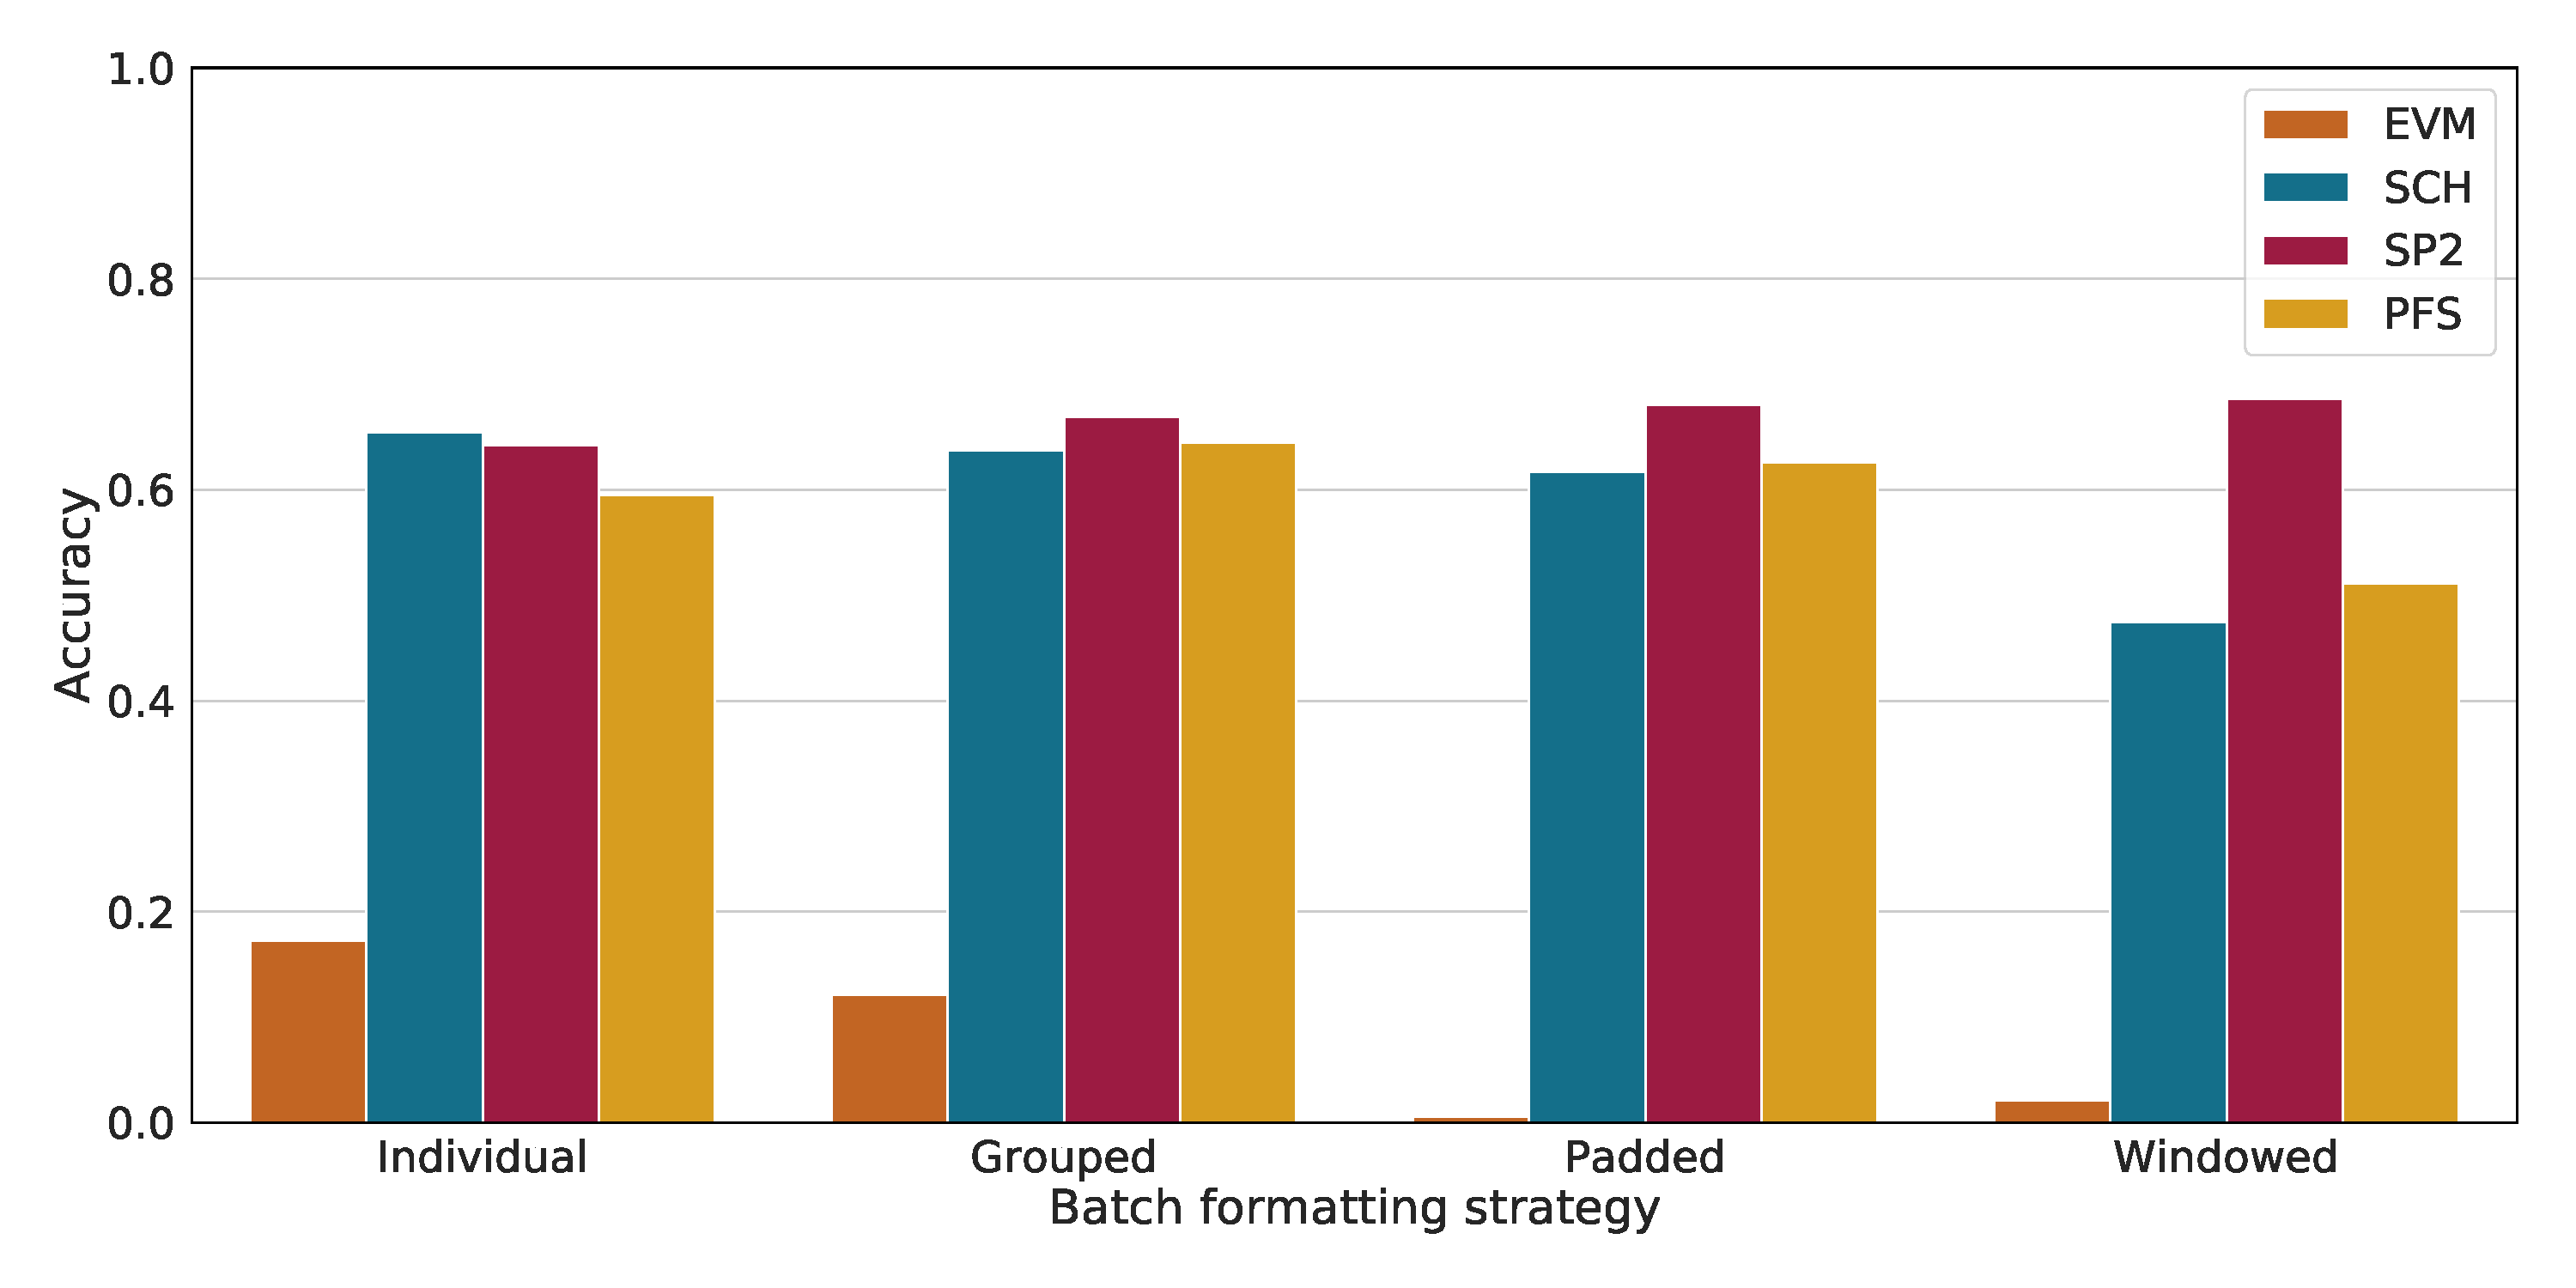
\includegraphics[width=\textwidth]{gfx/bpic2015_5/accuracies.pdf}
    \caption{Best accuracies on the validation set of BPIC15-5}
    \label{fig:max-accuracies-bpic2015-5}
\end{figure}
\FloatBarrier
\paragraph{Accuracy on BPIC11}
The most complex process is captured by BPIC11.
The validation accuracies that we obtained for this log are depicted in \autoref{fig:max-accuracies-bpic2011}.

Again, the EVM model shows subpar accuracies below $0.2$ across all batching strategies.
The SCH, SP2 and PFS models are very similar on the grouping and padding strategies, with all accuracies above $0.6$.
Only with the individual strategy does the SP2 model show a severe accuracy degradation.
On this strategy, the SCH model gives the highest accuracy with $0.682$.

\begin{figure}[!htb]
    \centering
    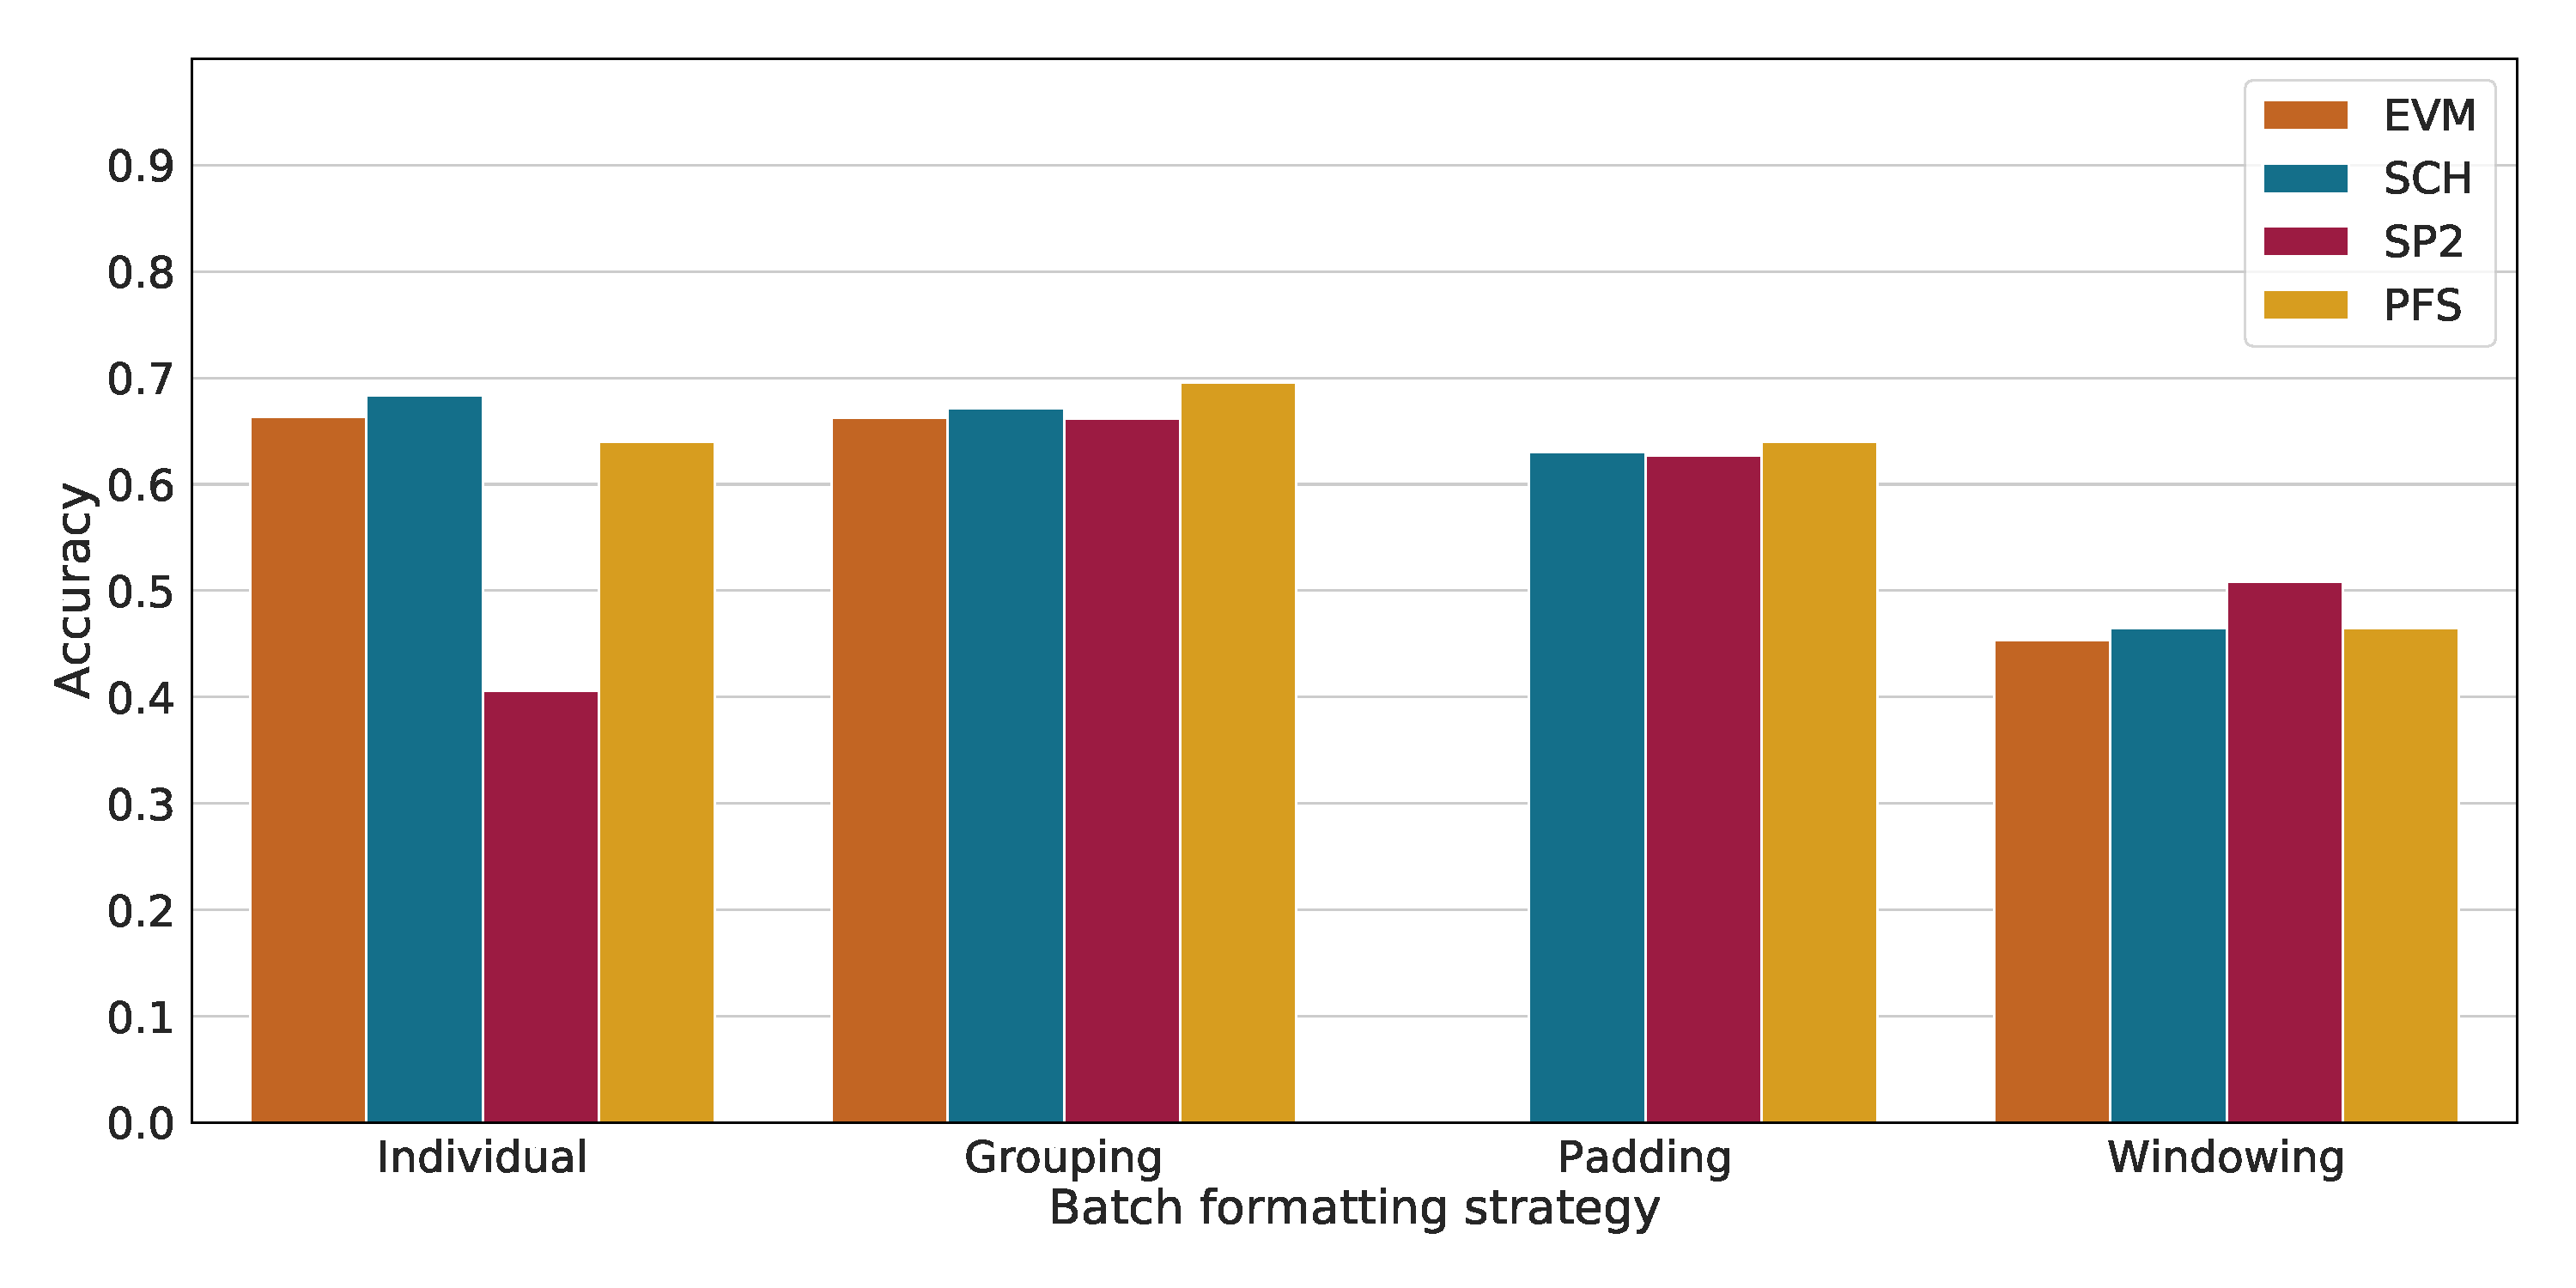
\includegraphics[width=\textwidth]{gfx/bpic2011/accuracies.pdf}
    \caption{Best accuracies on the validation set of BPIC11}
    \label{fig:max-accuracies-bpic2011}
\end{figure}

\paragraph{Verdict on accuracy}
Looking at the accuracy across all datasets, we detected five commonalities:

First, the batching strategies that supply the complete trace to the model lead to very similar results.

Second, the grouping strategy benefits high accuracies.
The mean of the top accuracies of the SCH, SP2 and PFS models on different batching strategies shows this in \autoref{tab:strategy-top-accuracies}.
The mean value is often the highest with the grouping strategy.
On BPIC12 however, the grouping strategy delivers relatively low accuracies.
We attribute the drop in accuracy to the large batch sizes that the strategy produces (cf. \autoref{tab:dataset-characteristics}).

Third, the windowing strategy always results in underperforming models.
Nonetheless, the SP2 model was able to cope with this strategy in the most efficient way, almost reaching maximum accuracies on BPIC15.

Fourth, \autoref{tab:strategy-top-accuracies} on mean accuracies also reveals that the prediction accuracy goes down with increasing complexity of the process.
The models are most accurate on the HelpDesk log, and become more inaccurate toward BPIC11.

Fifth, the EVM model always produced very low accuracies.

This concludes the presentation of the accuracy results.
We continue with the presentation of the timing measurements in the following section.

\begin{table}
\centering
\begin{tabular}{lrrrr}
\textbf{Dataset}  &  \textbf{Individual} &  \textbf{Grouping} &   \textbf{Padding} &  \textbf{Windowing}\\
\midrule
\textbf{HelpDesk} &    0.855    &  0.844    &  0.832    &  0.685    \\
\textbf{BPIC12  } &    0.850    &  0.761    &  0.833    &  0.728    \\
\textbf{BPIC15-1} &    0.614    &  0.670    &  0.635    &  0.559    \\
\textbf{BPIC15-2} &    0.577    &  0.604    &  0.581    &  0.503    \\
\textbf{BPIC15-3} &    0.649    &  0.680    &  0.654    &  0.581    \\
\textbf{BPIC15-4} &    0.638    &  0.668    &  0.645    &  0.579    \\
\textbf{BPIC15-5} &    0.630    &  0.650    &  0.640    &  0.557    \\
\textbf{BPIC11  } &    0.576    &  0.676    &  0.632    &  0.479    \\
\end{tabular}
\caption[Grouping strategy leads to best mean accuracies]{Accuracy means across the top accuracies of the SCH, SP2 and PFS models. The grouping strategy is generally the highest}
\label{tab:strategy-top-accuracies}
\end{table}
\FloatBarrier

\section{Training time}\label{sec:eval:training-time}
The training time that a model requires for an epoch is important to gauge the efficiency of its training process.
As in the previous section, we discuss the measurements per log and finish with a verdict.
For each log, a plot is shown that presents the training time per model, grouped by batching strategy.
The plots do not share the same scale on the y-axis.
During the following paragraphs, it is important to keep in mind that the batch size has a direct effect on the training time since it corresponds to the number of weight adjustments that need to be calculated.

\paragraph{Training times on HelpDesk}
How long training an epoch took with a model and a particular strategy on the HelpDesk log is shown in \autoref{fig:helpdesk-training-timings}.
Training with the grouping strategy takes the least amount of time and the most with the individual strategy.
The timings are very similar for all models on the same strategy.

\begin{figure}[!htb]
    \centering
    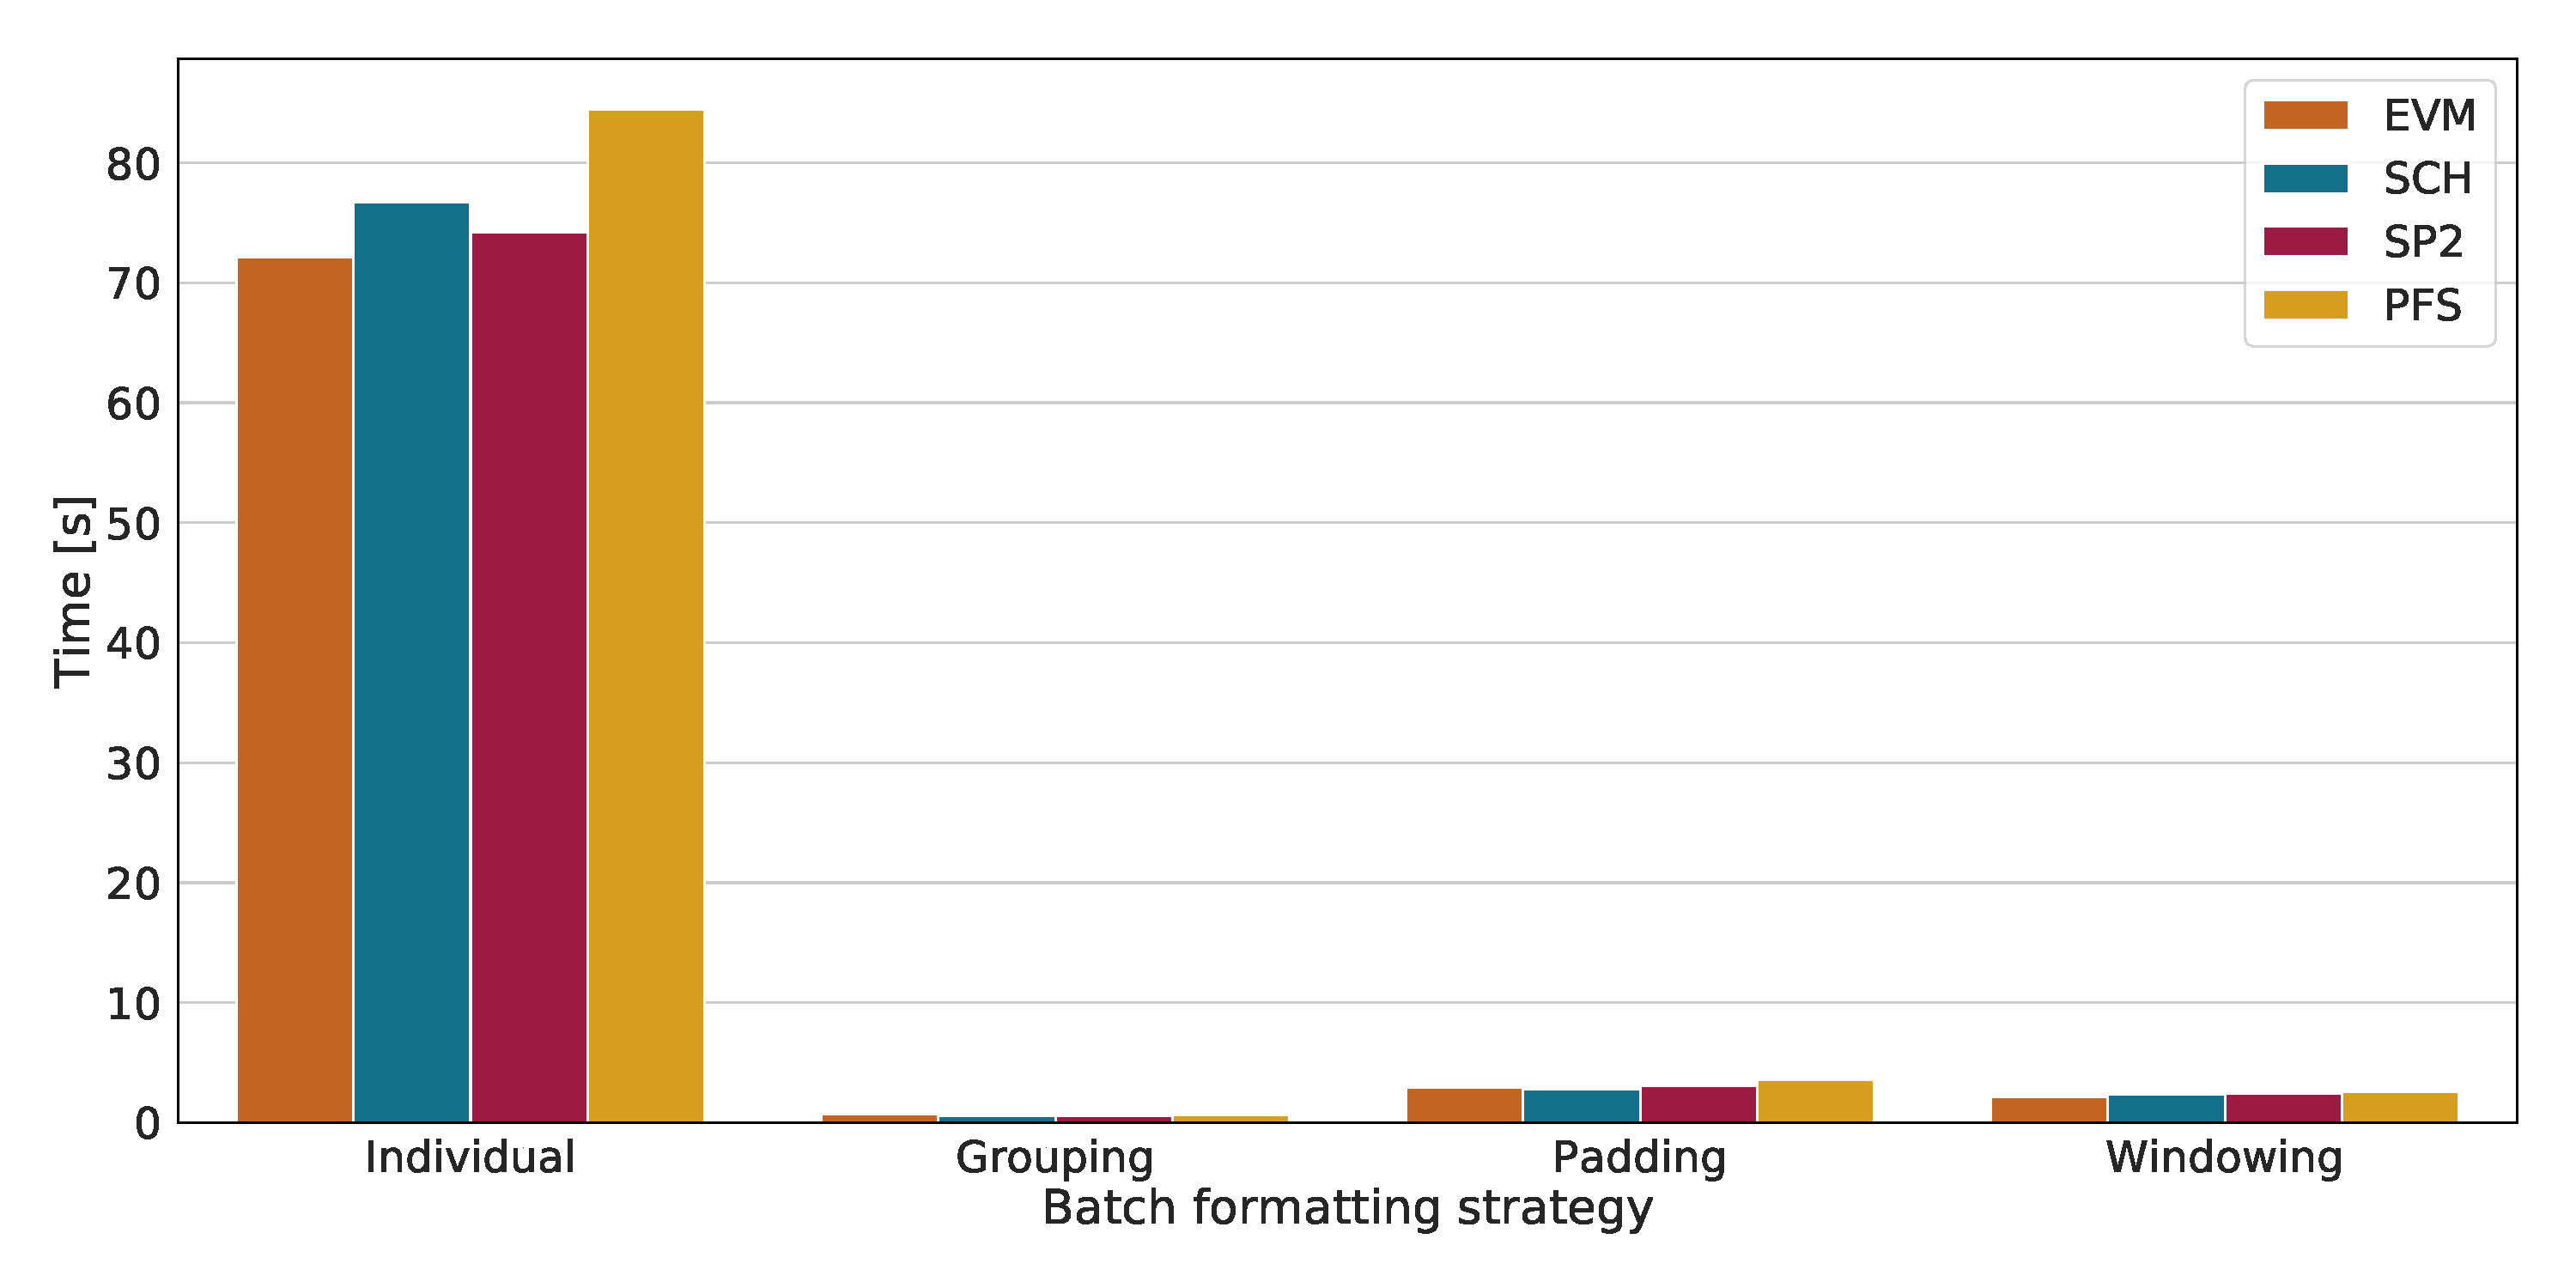
\includegraphics[width=\textwidth]{gfx/helpdesk/train_timings.pdf}
    \caption{Training times measured on HelpDesk}
    \label{fig:helpdesk-training-timings}
\end{figure}

\paragraph{Training times on BPIC12}
\autoref{fig:BPIC12-training-timings} depicts the epoch training times for BPIC12.
As for the HelpDesk log, the timings for models on the same strategy are very similar.
By far, they are the highest for each model on the individual strategy at approximately 10 minutes.
The other strategies take significantly less time.

\begin{figure}[!htb]
    \centering
    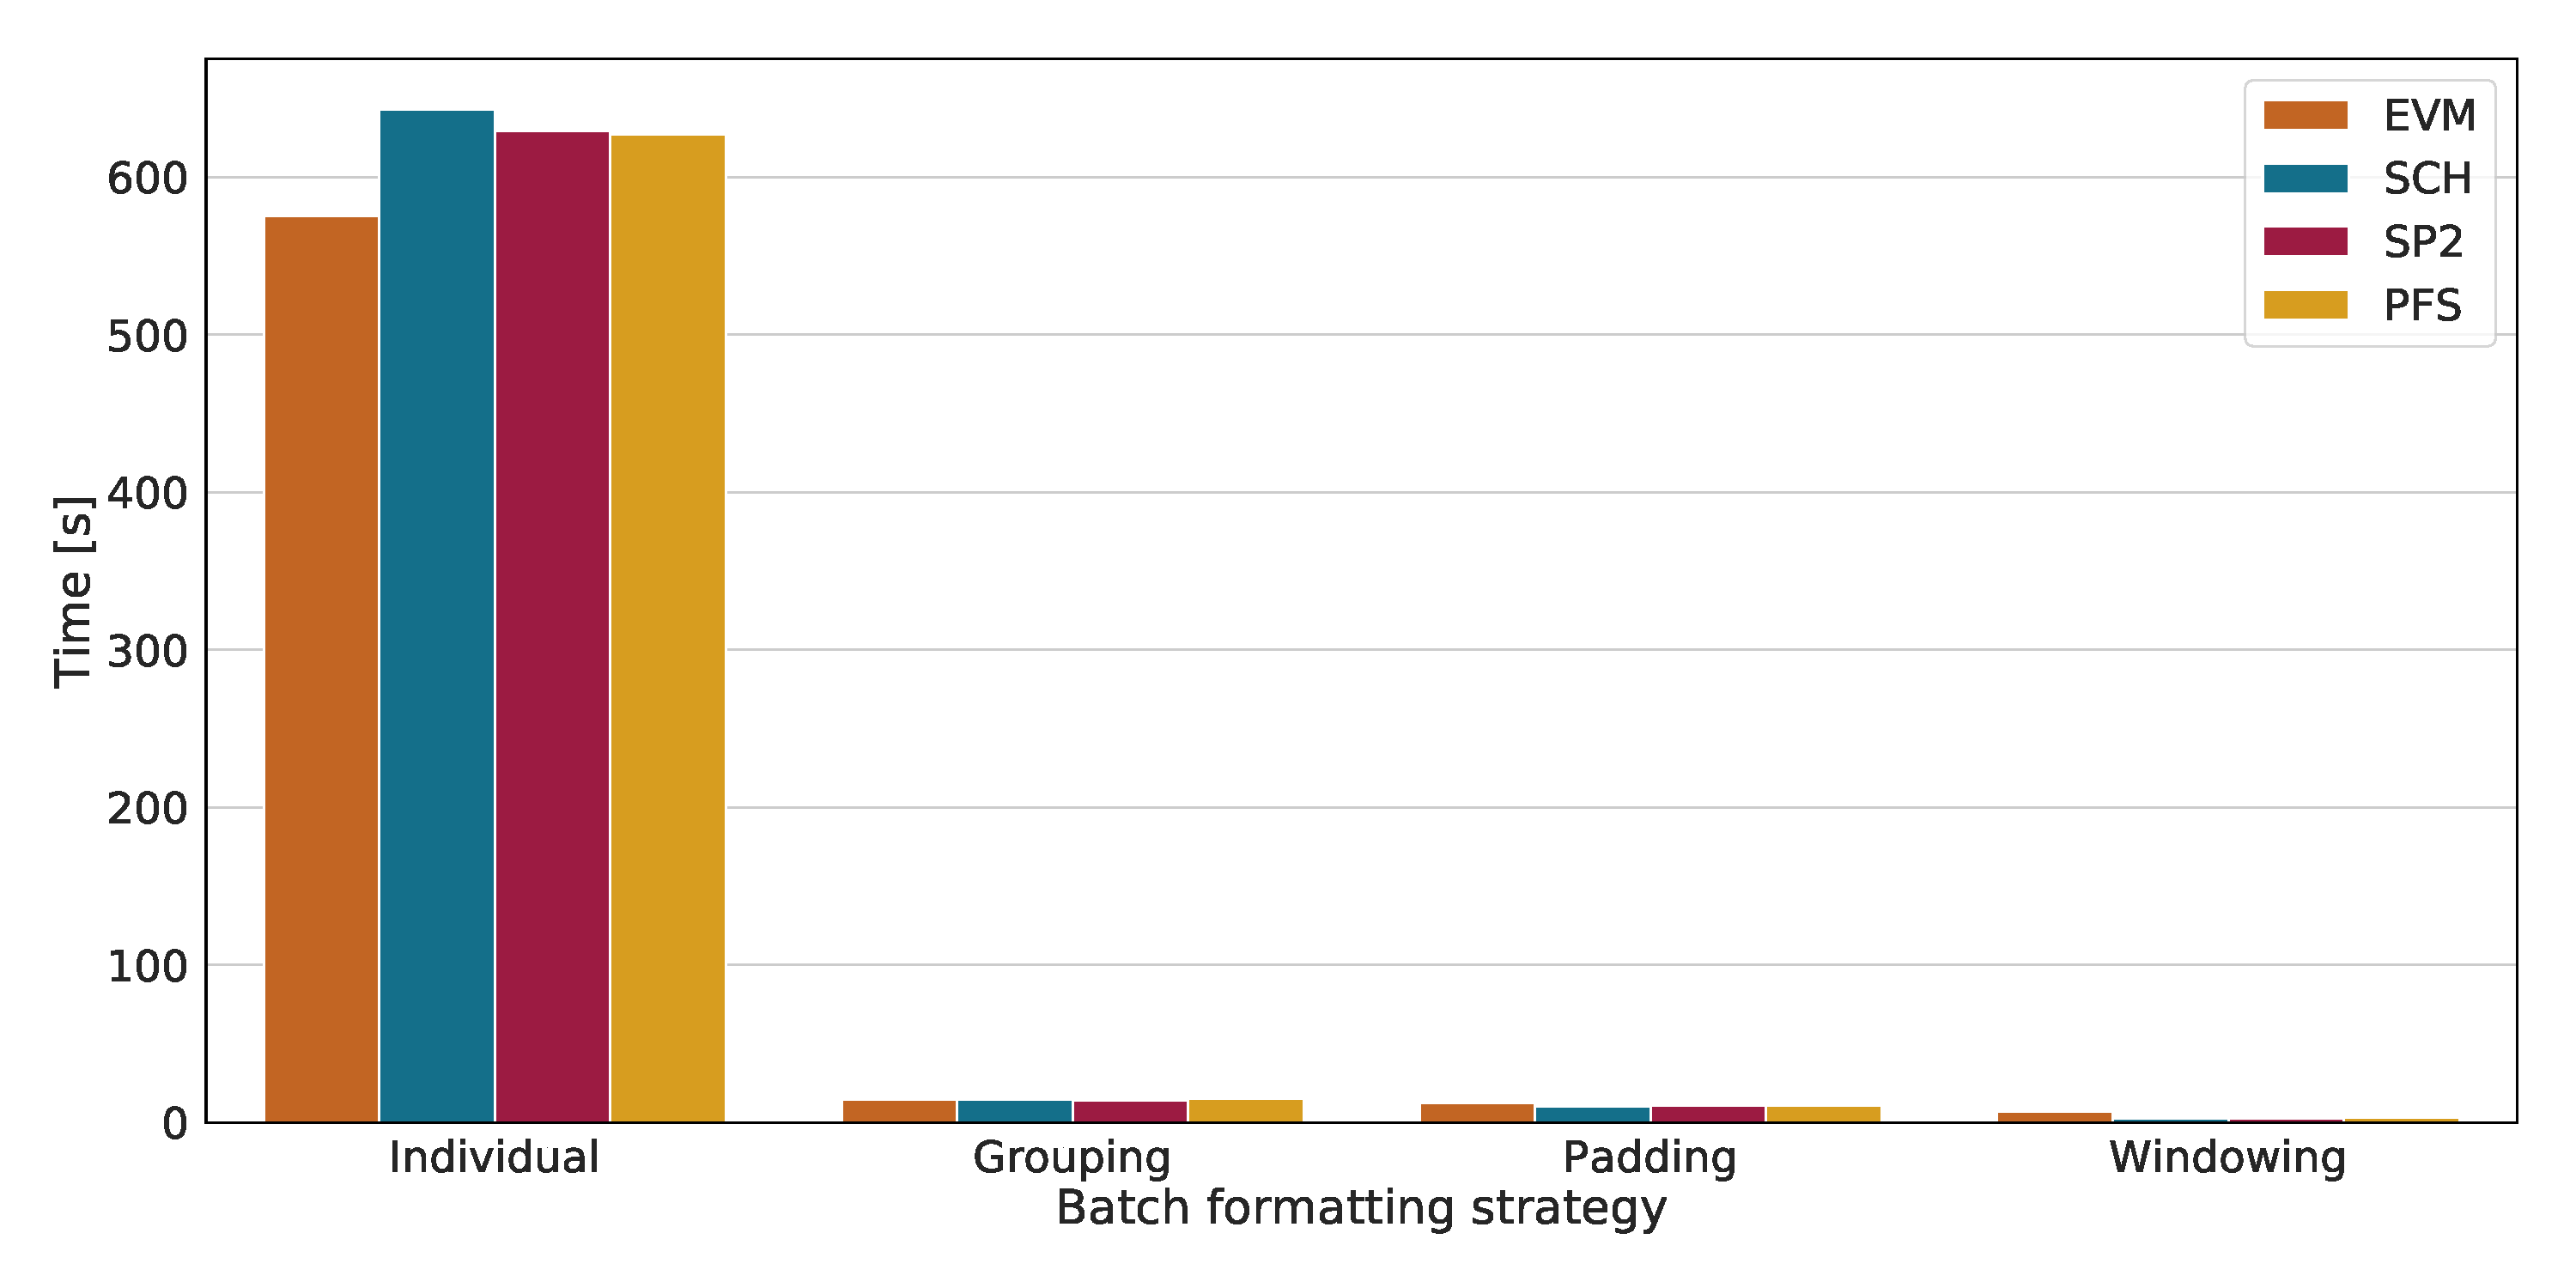
\includegraphics[width=\textwidth]{gfx/bpic2012/train_timings.pdf}
    \caption{Training times measured on BPIC12}
    \label{fig:BPIC12-training-timings}
\end{figure}

\paragraph{Training times on BPIC15}
The training timings taken during the model training on the BPIC15 log are shown in \autoref{fig:BPIC15-1-training-timings} to \autoref{fig:BPIC15-5-training-timings}.
The measurements are very similar across the five datasets in the log, which is why we explain them in a collective fashion.

The SCH, SP2 and PFS models always need a very similar amount of training time per epoch.
The EVM model often needs less than half that time.
Across all five datasets, it is also possible to see that the individual strategy takes by far the most time.
Significantly less time is needed by the padding strategy, although it still ranks third.
The grouping strategy needs a little less time, and the windowing strategy trains fastest by far.

\begin{figure}[!htb]
    \centering
    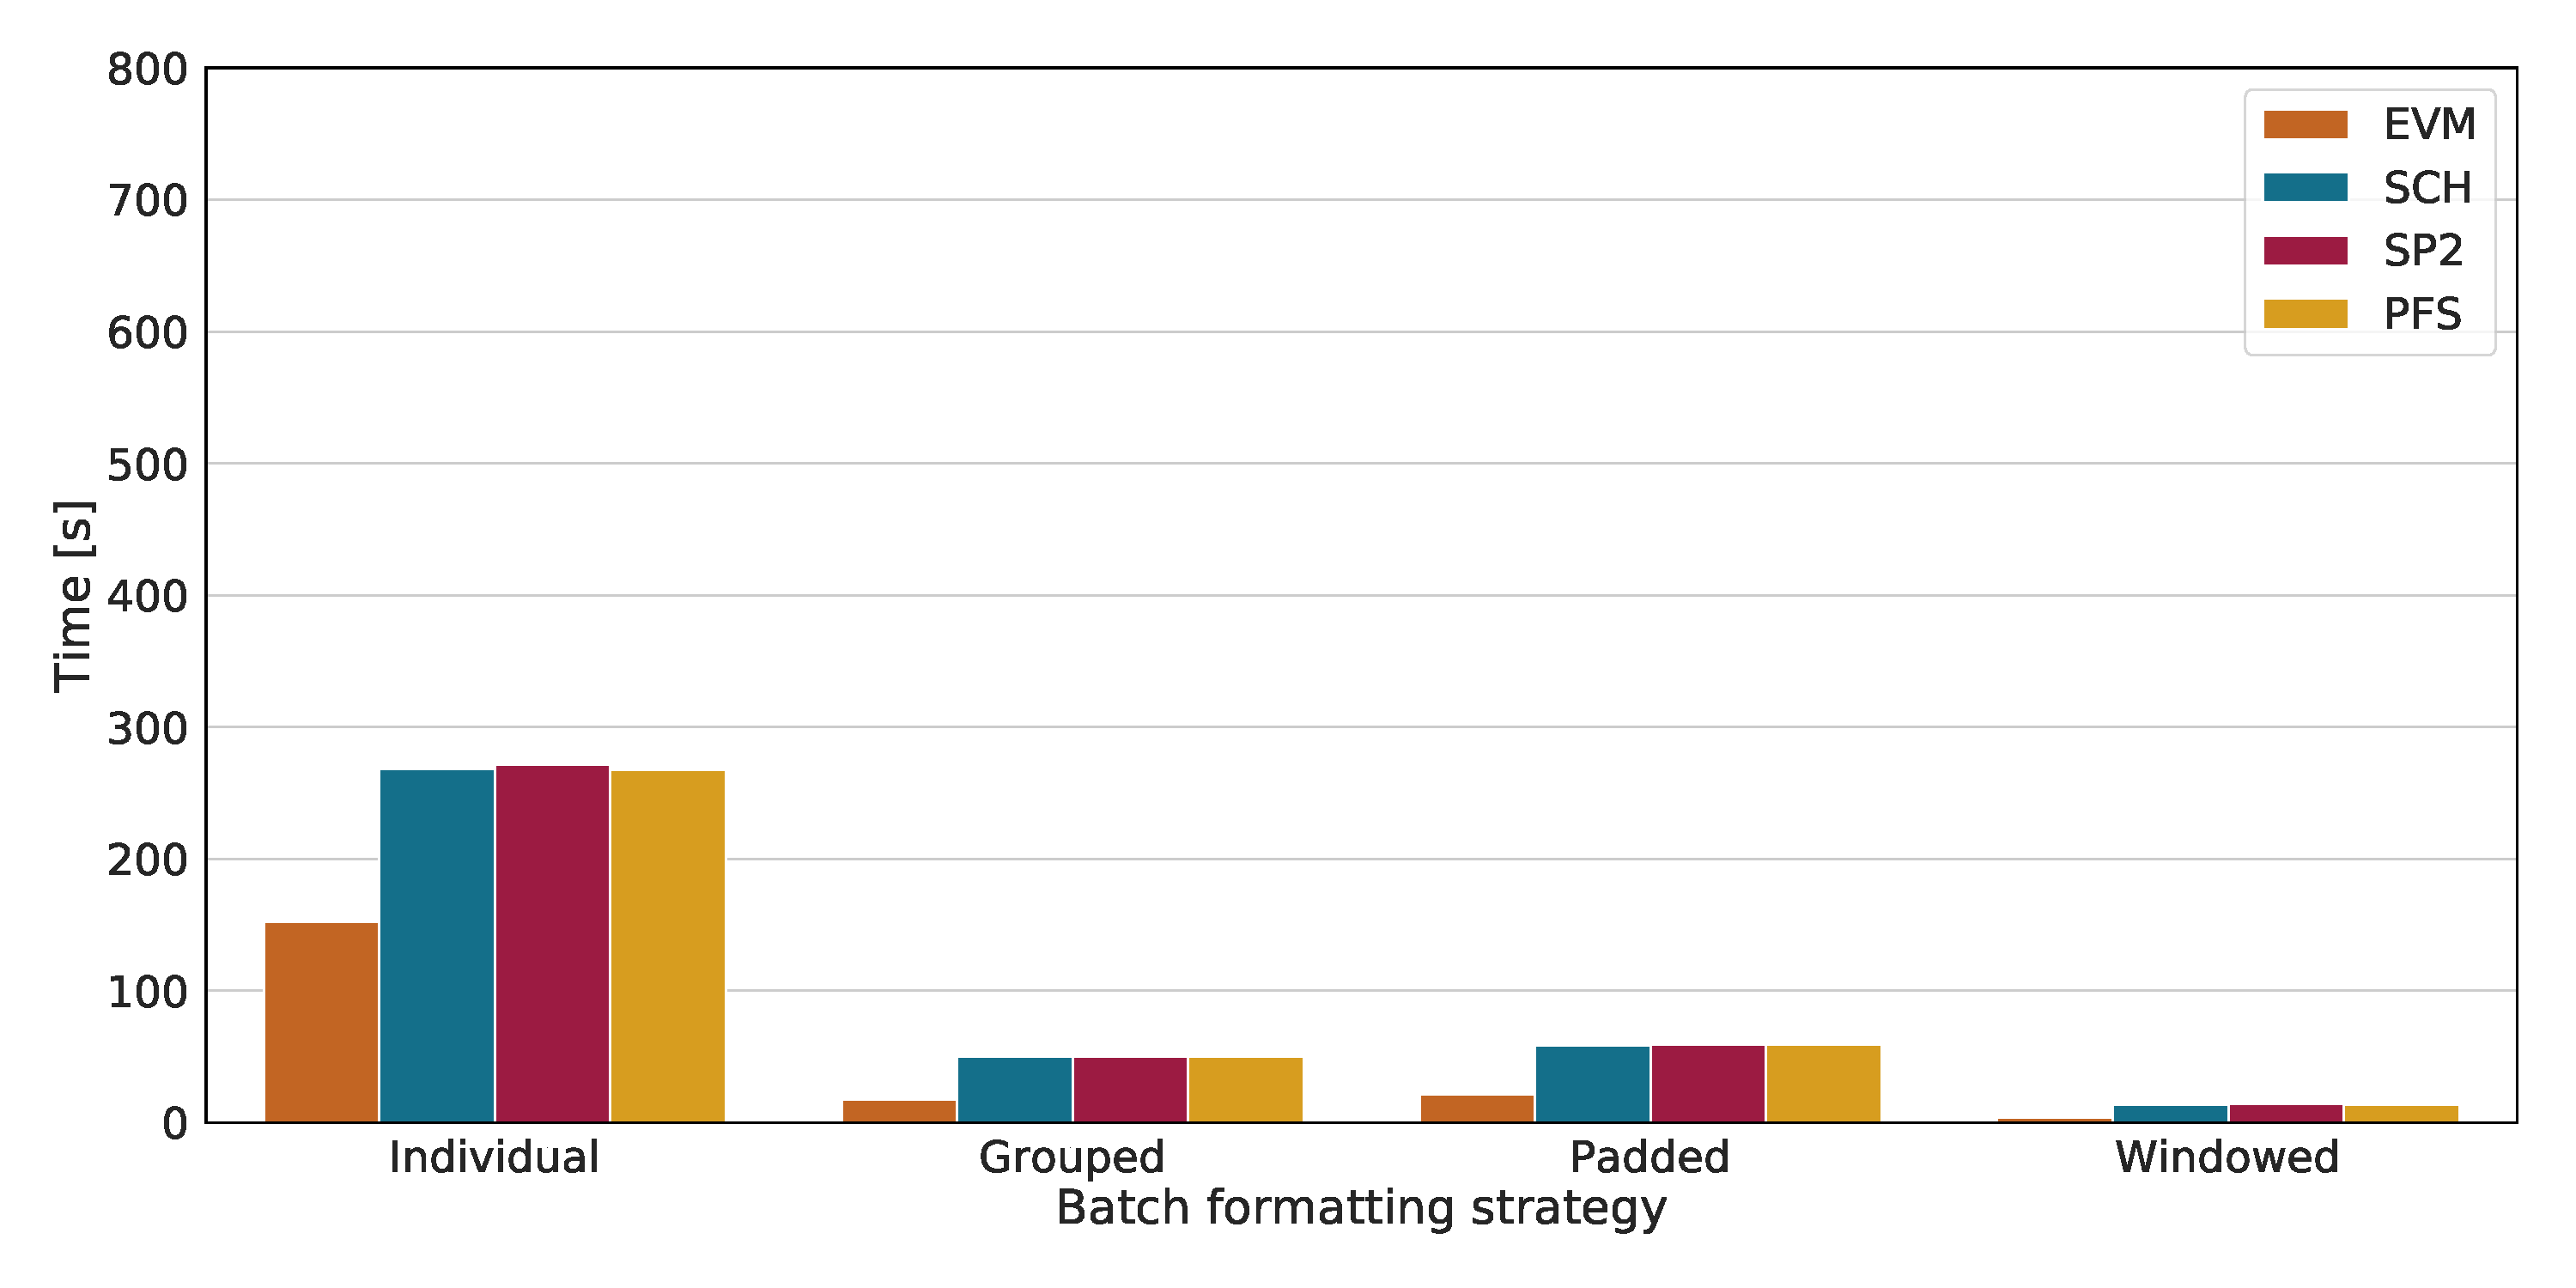
\includegraphics[width=\textwidth]{gfx/bpic2015_1/train_timings.pdf}
    \caption{Training times measured on BPIC15-1}
    \label{fig:BPIC15-1-training-timings}
\end{figure}
\begin{figure}[!htb]
    \centering
    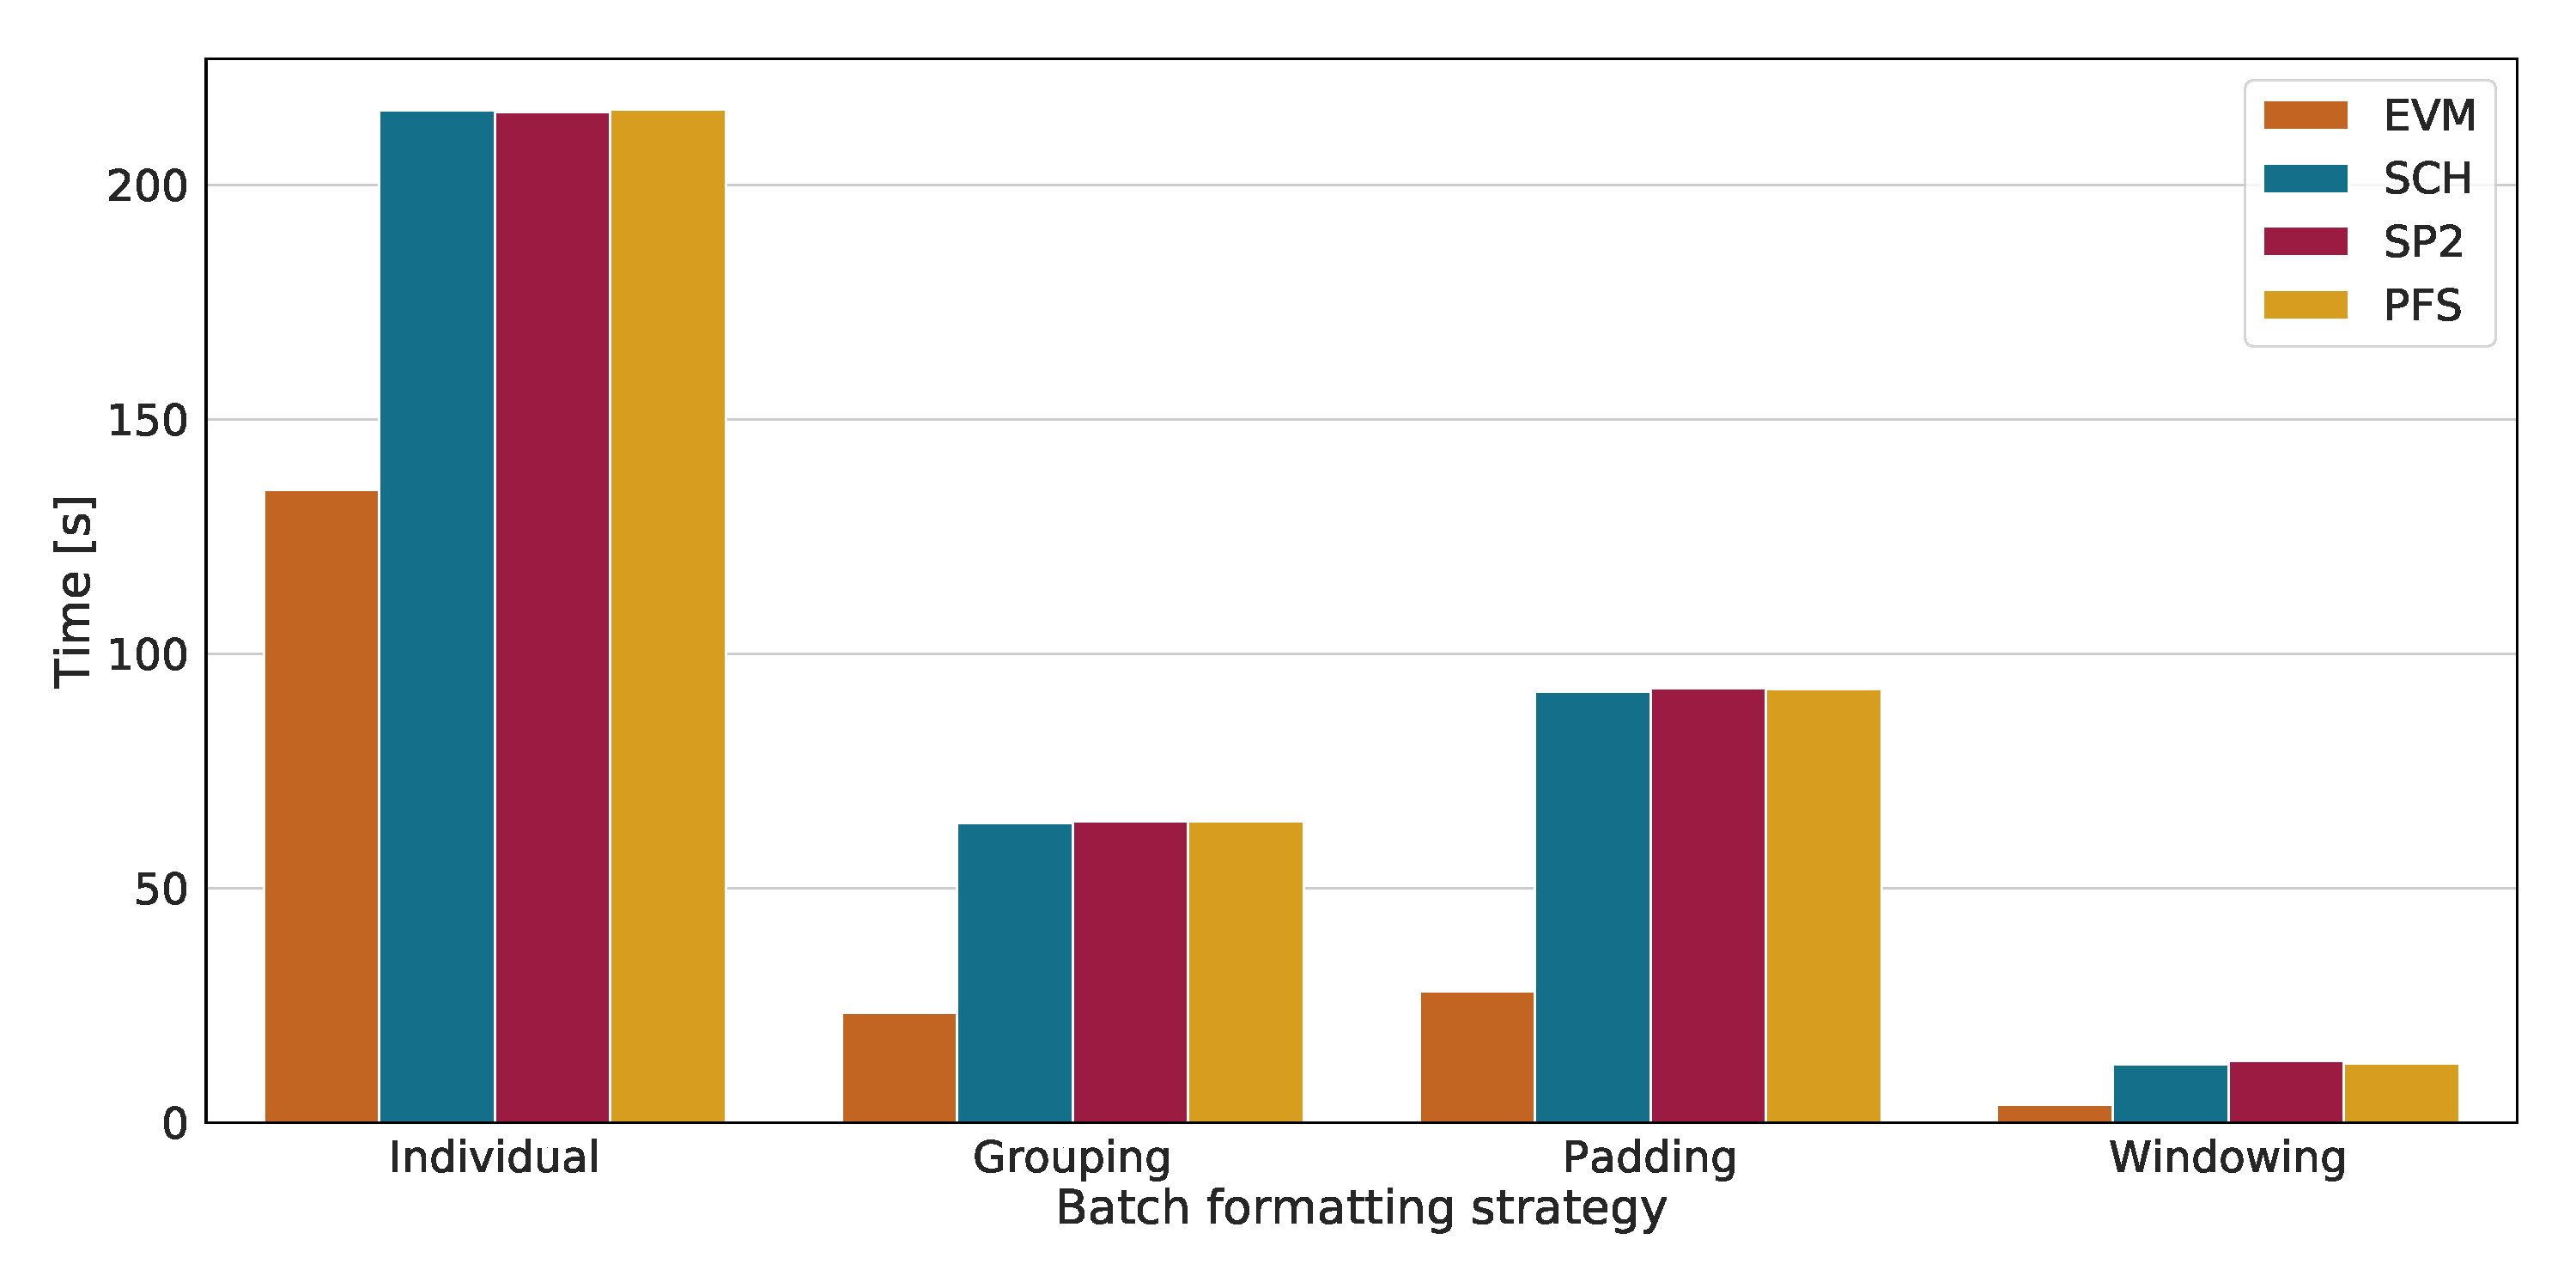
\includegraphics[width=\textwidth]{gfx/bpic2015_2/train_timings.pdf}
    \caption{Training times measured on BPIC15-2}
    \label{fig:BPIC15-2-training-timings}
\end{figure}
\begin{figure}[!htb]
    \centering
    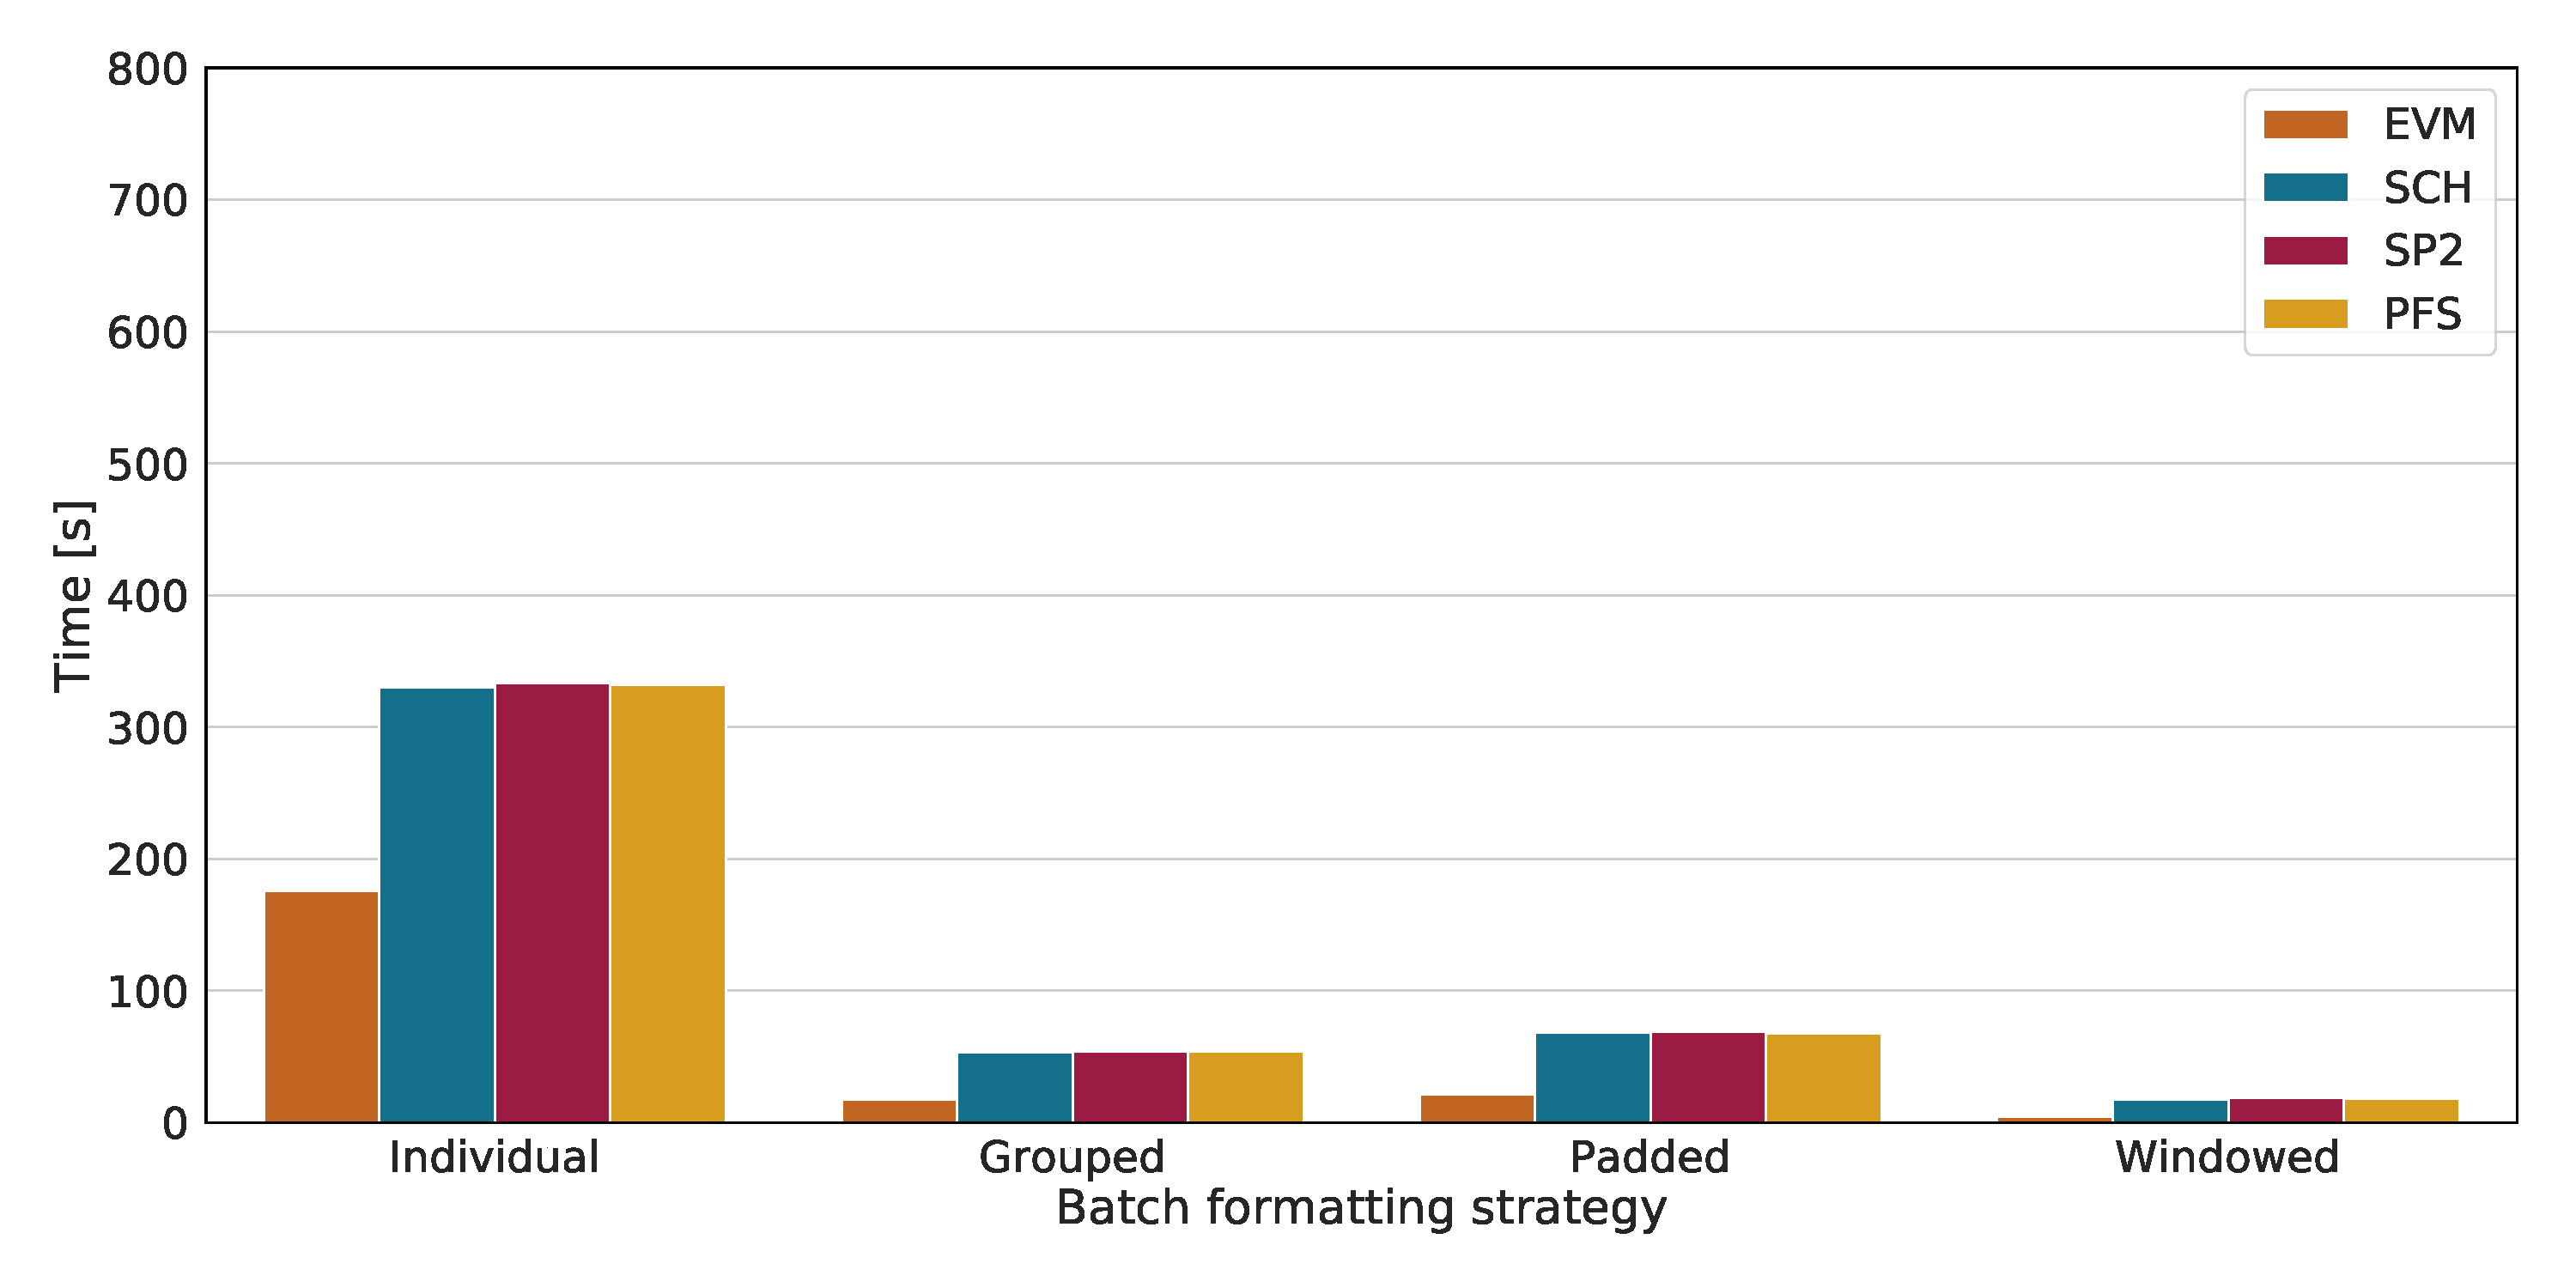
\includegraphics[width=\textwidth]{gfx/bpic2015_3/train_timings.pdf}
    \caption{Training times measured on BPIC15-3}
    \label{fig:BPIC15-3-training-timings}
\end{figure}
\begin{figure}[!htb]
    \centering
    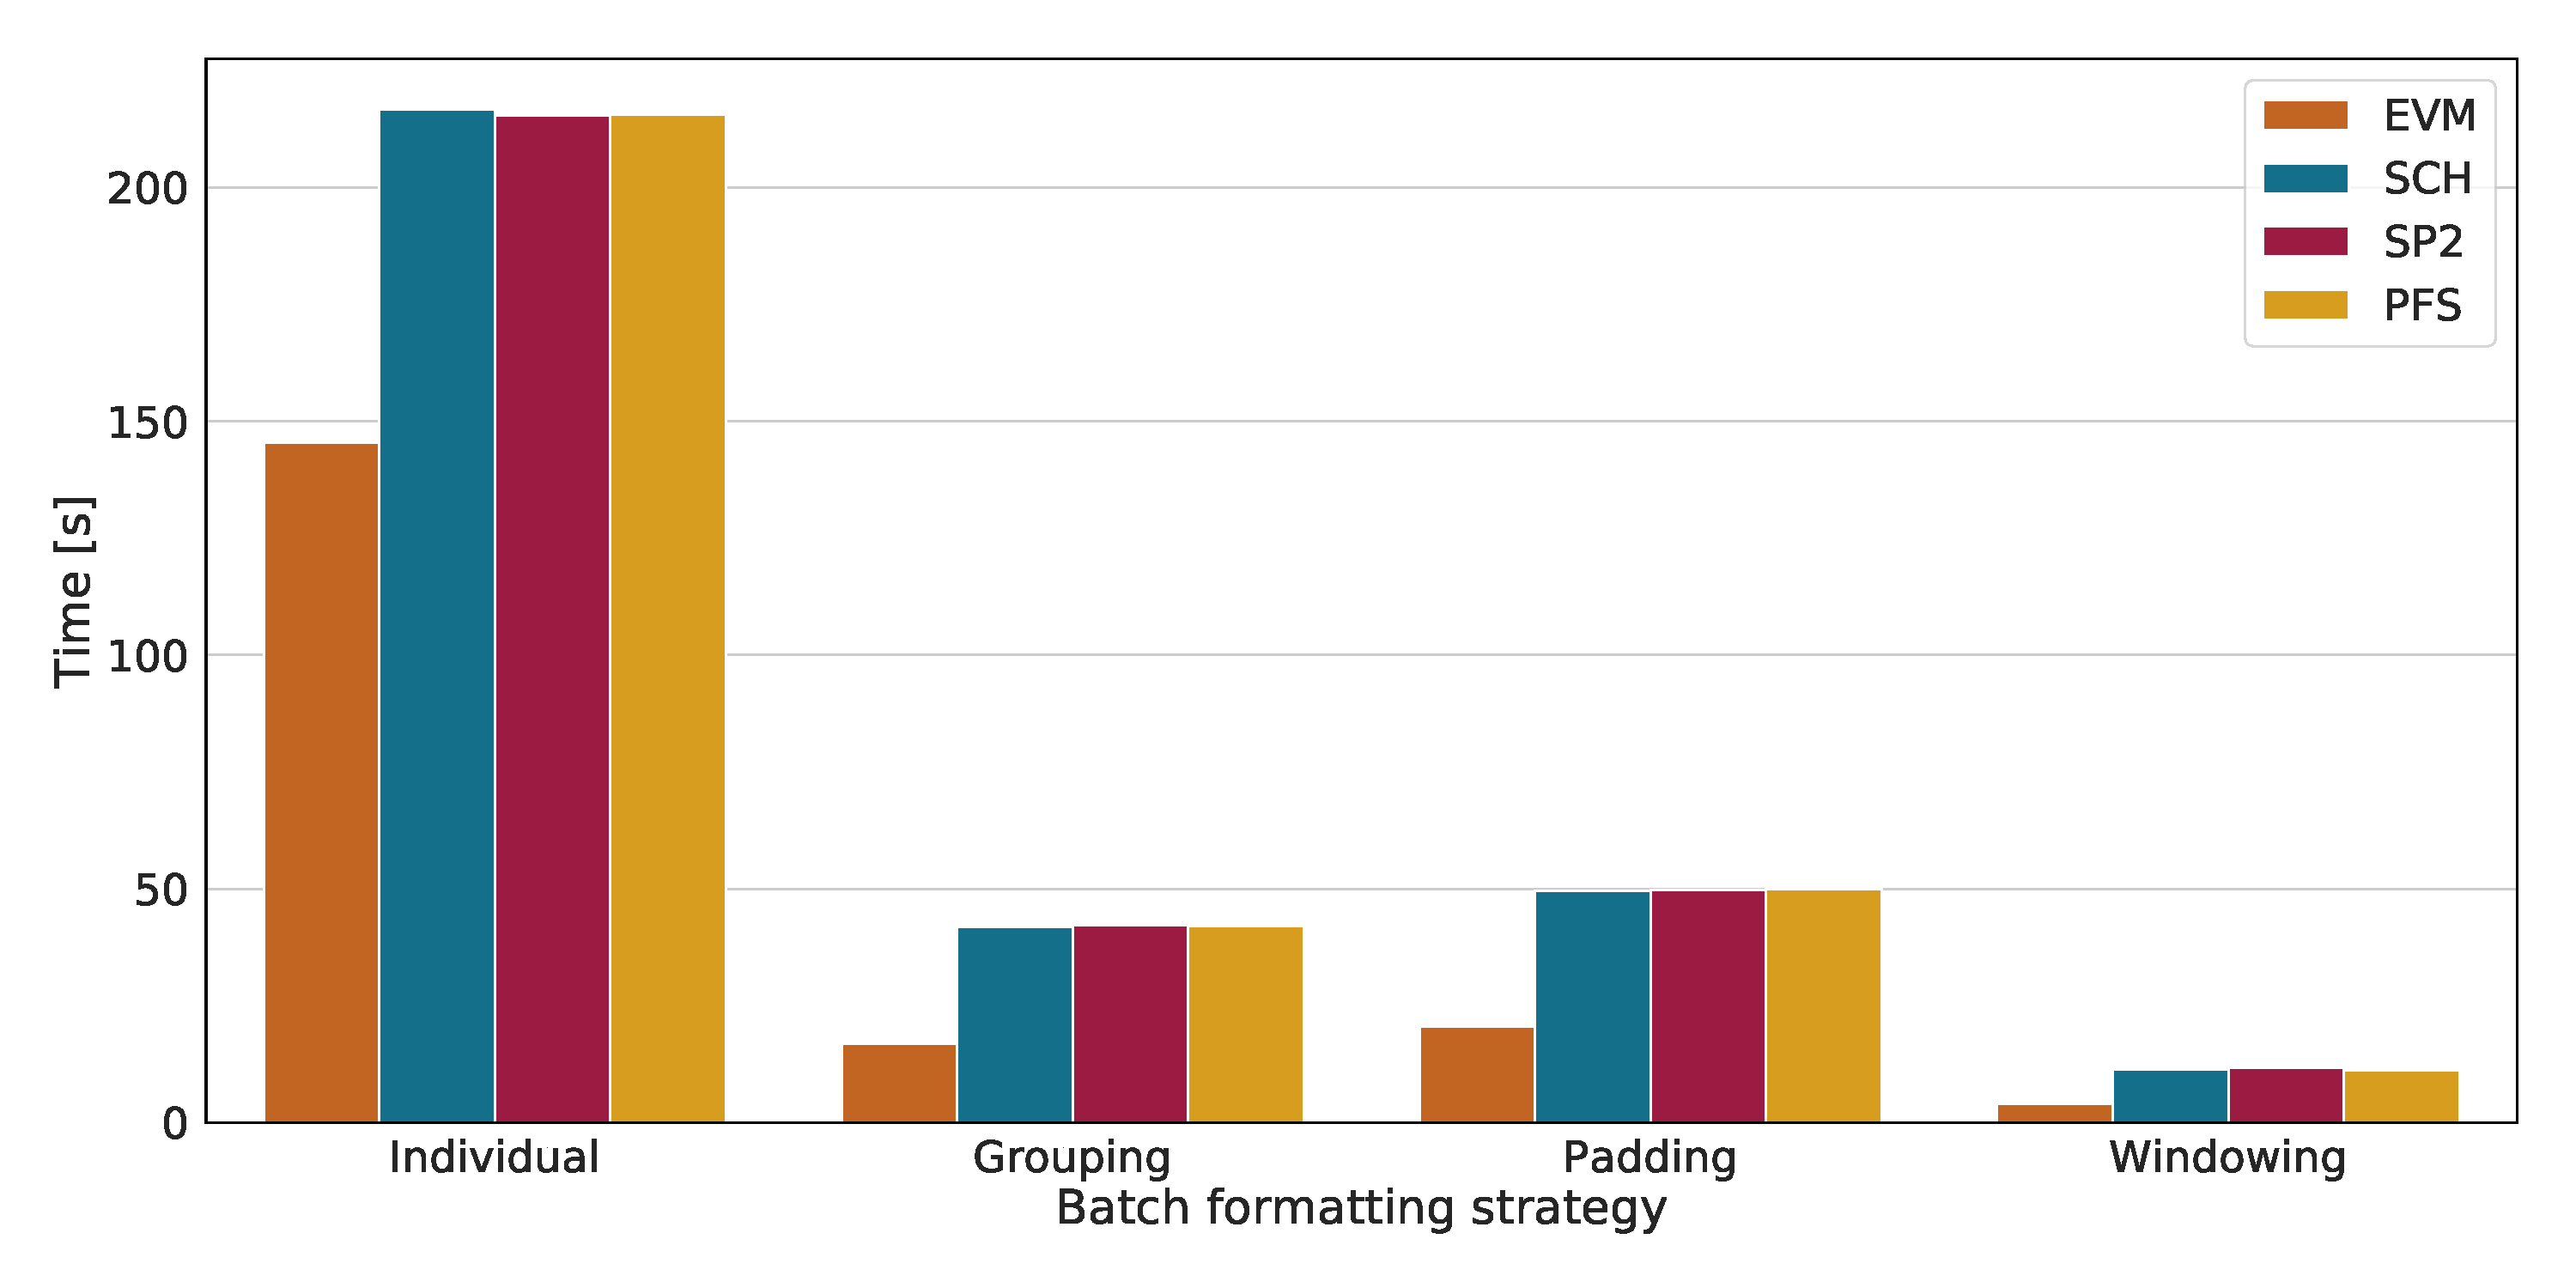
\includegraphics[width=\textwidth]{gfx/bpic2015_4/train_timings.pdf}
    \caption{Training times measured on BPIC15-4}
    \label{fig:BPIC15-4-training-timings}
\end{figure}
\begin{figure}[!htb]
    \centering
    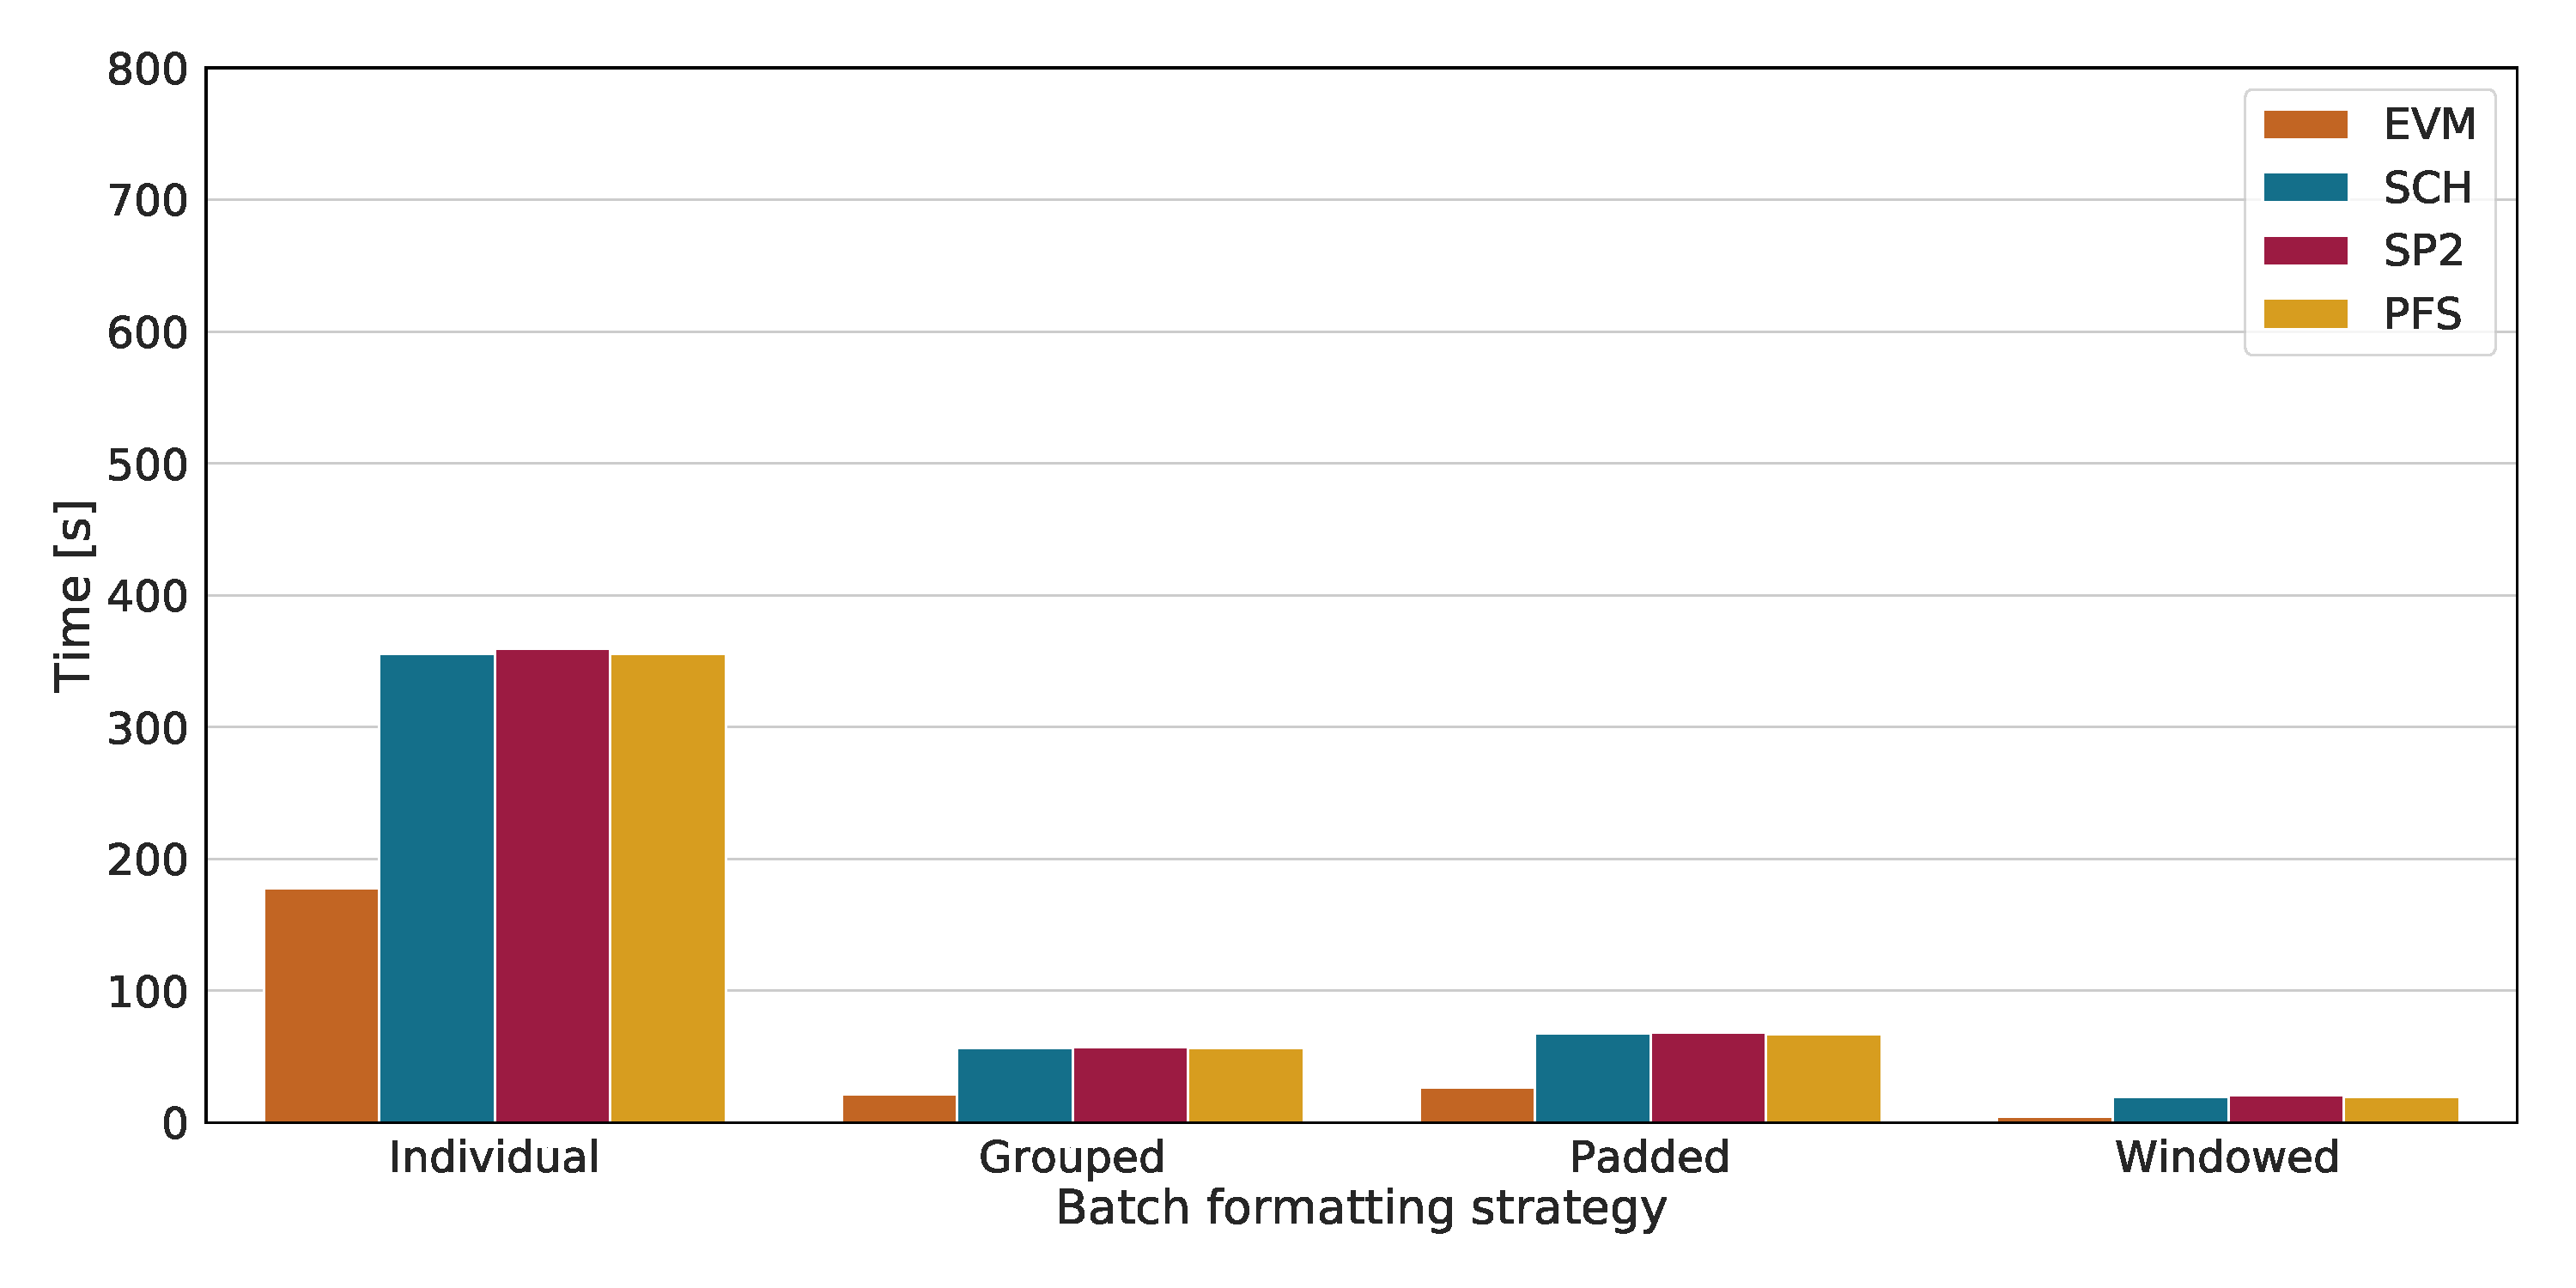
\includegraphics[width=\textwidth]{gfx/bpic2015_5/train_timings.pdf}
    \caption{Training times measured on BPIC15-5}
    \label{fig:BPIC15-5-training-timings}
\end{figure}
\FloatBarrier
\newpage
\paragraph{Training times on BPIC11}
\autoref{fig:BPIC11-training-timings} shows the training times measured on BPIC11.
On this plot, it is visible that the EVM model takes approximately half the training time of the other models.
As before, the other models require about the same time for an epoch for the same batching strategy.
The individual strategy causes the longest epochs, shortened a little by the grouping strategy.
The padding strategy incurs a big drop in training times, and the windowing strategy is the fastest, again.

\begin{figure}[!htb]
    \centering
    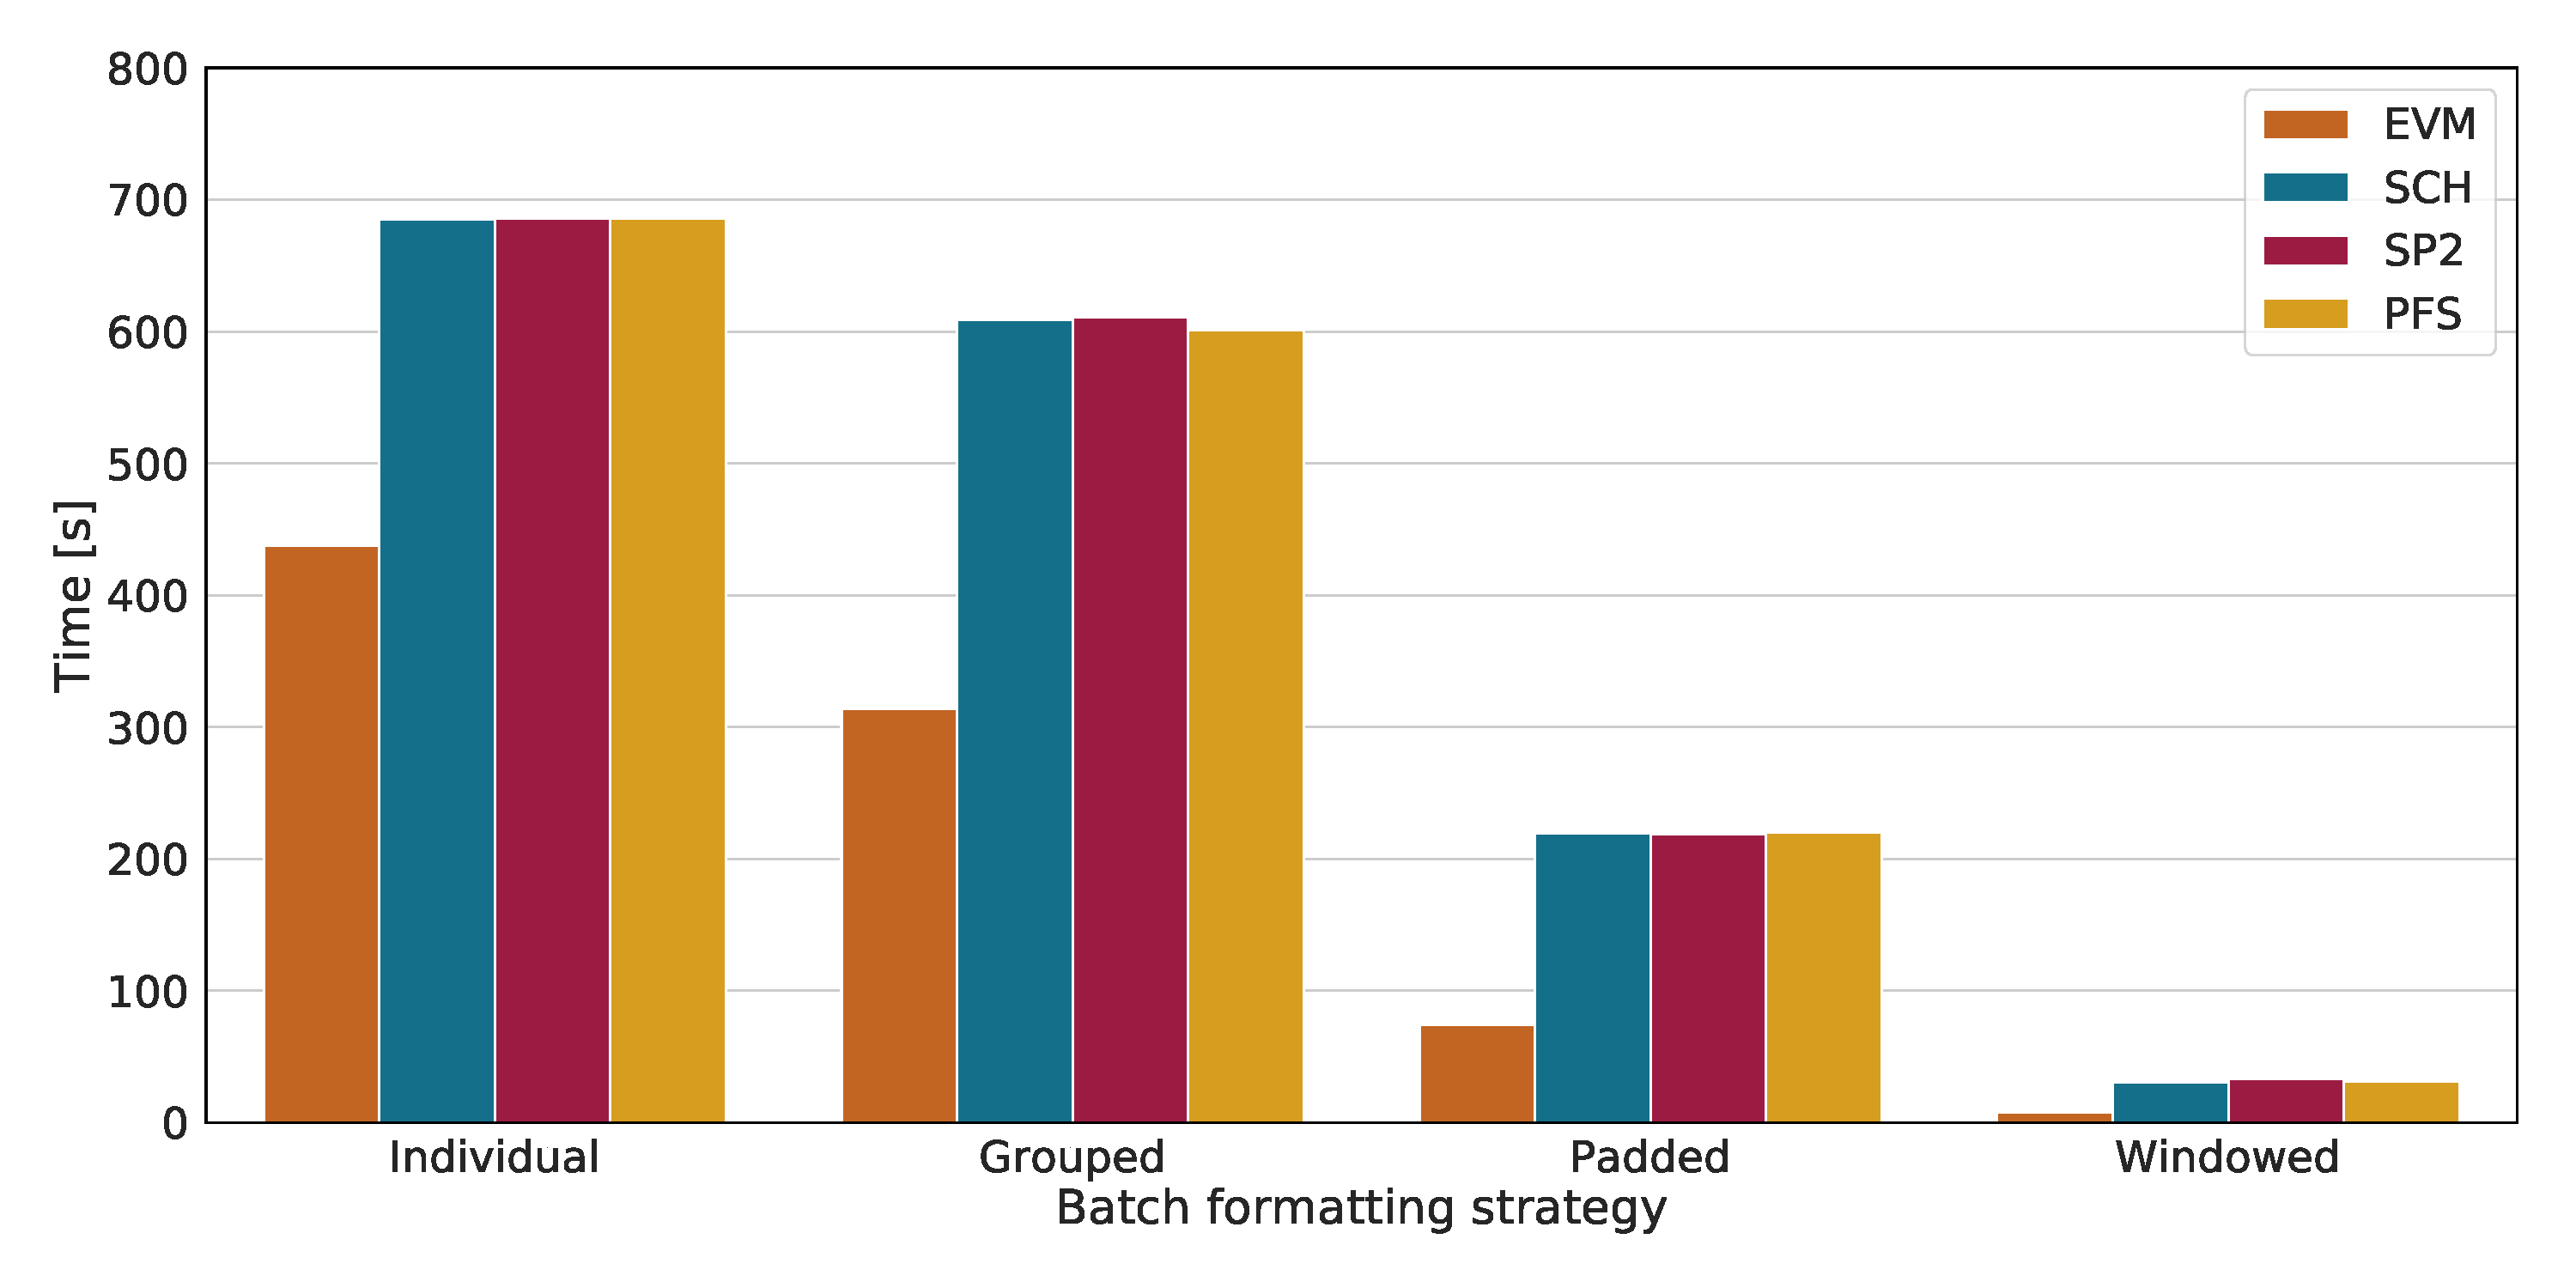
\includegraphics[width=\textwidth]{gfx/bpic2011/train_timings.pdf}
    \caption{Training times measured on BPIC11}
    \label{fig:BPIC11-training-timings}
\end{figure}

\paragraph{Verdict on training times}
Across all datasets, we gathered the following observations.
The individual strategy leads to the longest times overall.
This is not surprising, as \autoref{tab:dataset-characteristics} reveals that this strategy leads to hundreds of batches per epoch - more than any other strategy.
Each batch incurs a weight adjustment, which leads to additional required computing time.

The grouping strategy leads to significant reductions in training times, depending on how diverse the trace lengths are. \autoref{tab:dataset-characteristics} explains why the reduction is not as prominent with BPIC11: It exhibits up to 1814 different lengths, while the other datasets only exhibit $5\%$ to $10\%$ of this number.

With the padding strategy, it is possible to overcome the limitations imposed by trace lengths and construct batches out of any number of traces. This makes it easier to optimize the batch size, which can lead to faster training times.

Finally, the windowing strategy is the fastest.
It produces a constant number of timesteps and allows for arbitrary batch sizes.
The low number of timesteps additionally reduces the amount of calculation that needs to be done.
\FloatBarrier

\section{Stability}\label{sec:eval:stability}
As we stressed in the introduction, the stability of the prediction accuracy along the progress of a case can strongly impact the level of trust that users put into a model~\cite{metzger2015}.

In this section, we show the stability plots produced on each log, one for each batching strategy.
We discuss the logs in the order of increasing process complexity and finish with a verdict.
For space reasons, we only present the most informative graph per log in this section, and enclose the others in \autoref{appendix:evaluation-measurements}.

Each figure for a batching strategy and a dataset contains four curves, one for each model.
The curves show the model accuracy along the progression of all traces inside the validation set in steps of $5\%$.
The stability on the HelpDesk log was calculated in steps of $10\%$, as most cases in it are only 13 steps long.
The following paragraphs explain the curves in further detail.

\paragraph{Stability on HelpDesk}
On the HelpDesk log, it shows again that the batching strategies have a substantial impact on the accuracy in different stages.

\autoref{fig:helpdesk-individual-stability} shows the stability of each model with the individual strategy.
The four curves start around $0.8$ and then stay at that level until $60\%$ progress.
The EVM model becomes less and less accurate from the beginning.
At the $60\%$ mark, all curves show a small correction, before going up toward an accuracy of $1$ at the end.

\autoref{fig:helpdesk-grouped-stability}, \autoref{fig:helpdesk-padded-stability}, and \autoref{fig:helpdesk-windowed-stability} show the stability on the other strategies.
With the grouping strategy, the curves are very similar, except for the EVM curve.
The EVM accuracy curve starts at around $0.05$ and goes toward $1$ at the end of the trace.

The padding strategy makes all four models very unstable.
After the SCH, SP2 and PFS curves start around $0.8$, the curves see degradations and fluctuation around the $50\%$ mark, with the PFS model completely failing at $0$ accuracy at the end.
The EVM model starts at an accuracy of $0$ and rises to $1$ at the end of all traces.

The windowing strategy makes the curves very jittery.
All curves start at 0 accuracy and stay below $0.5$ accuracy until $60\%$ progress.
At this point, the curves shoot up above $0.8$ and finish at an accuracy of $1$.

\begin{figure}[!htb]
    \centering
    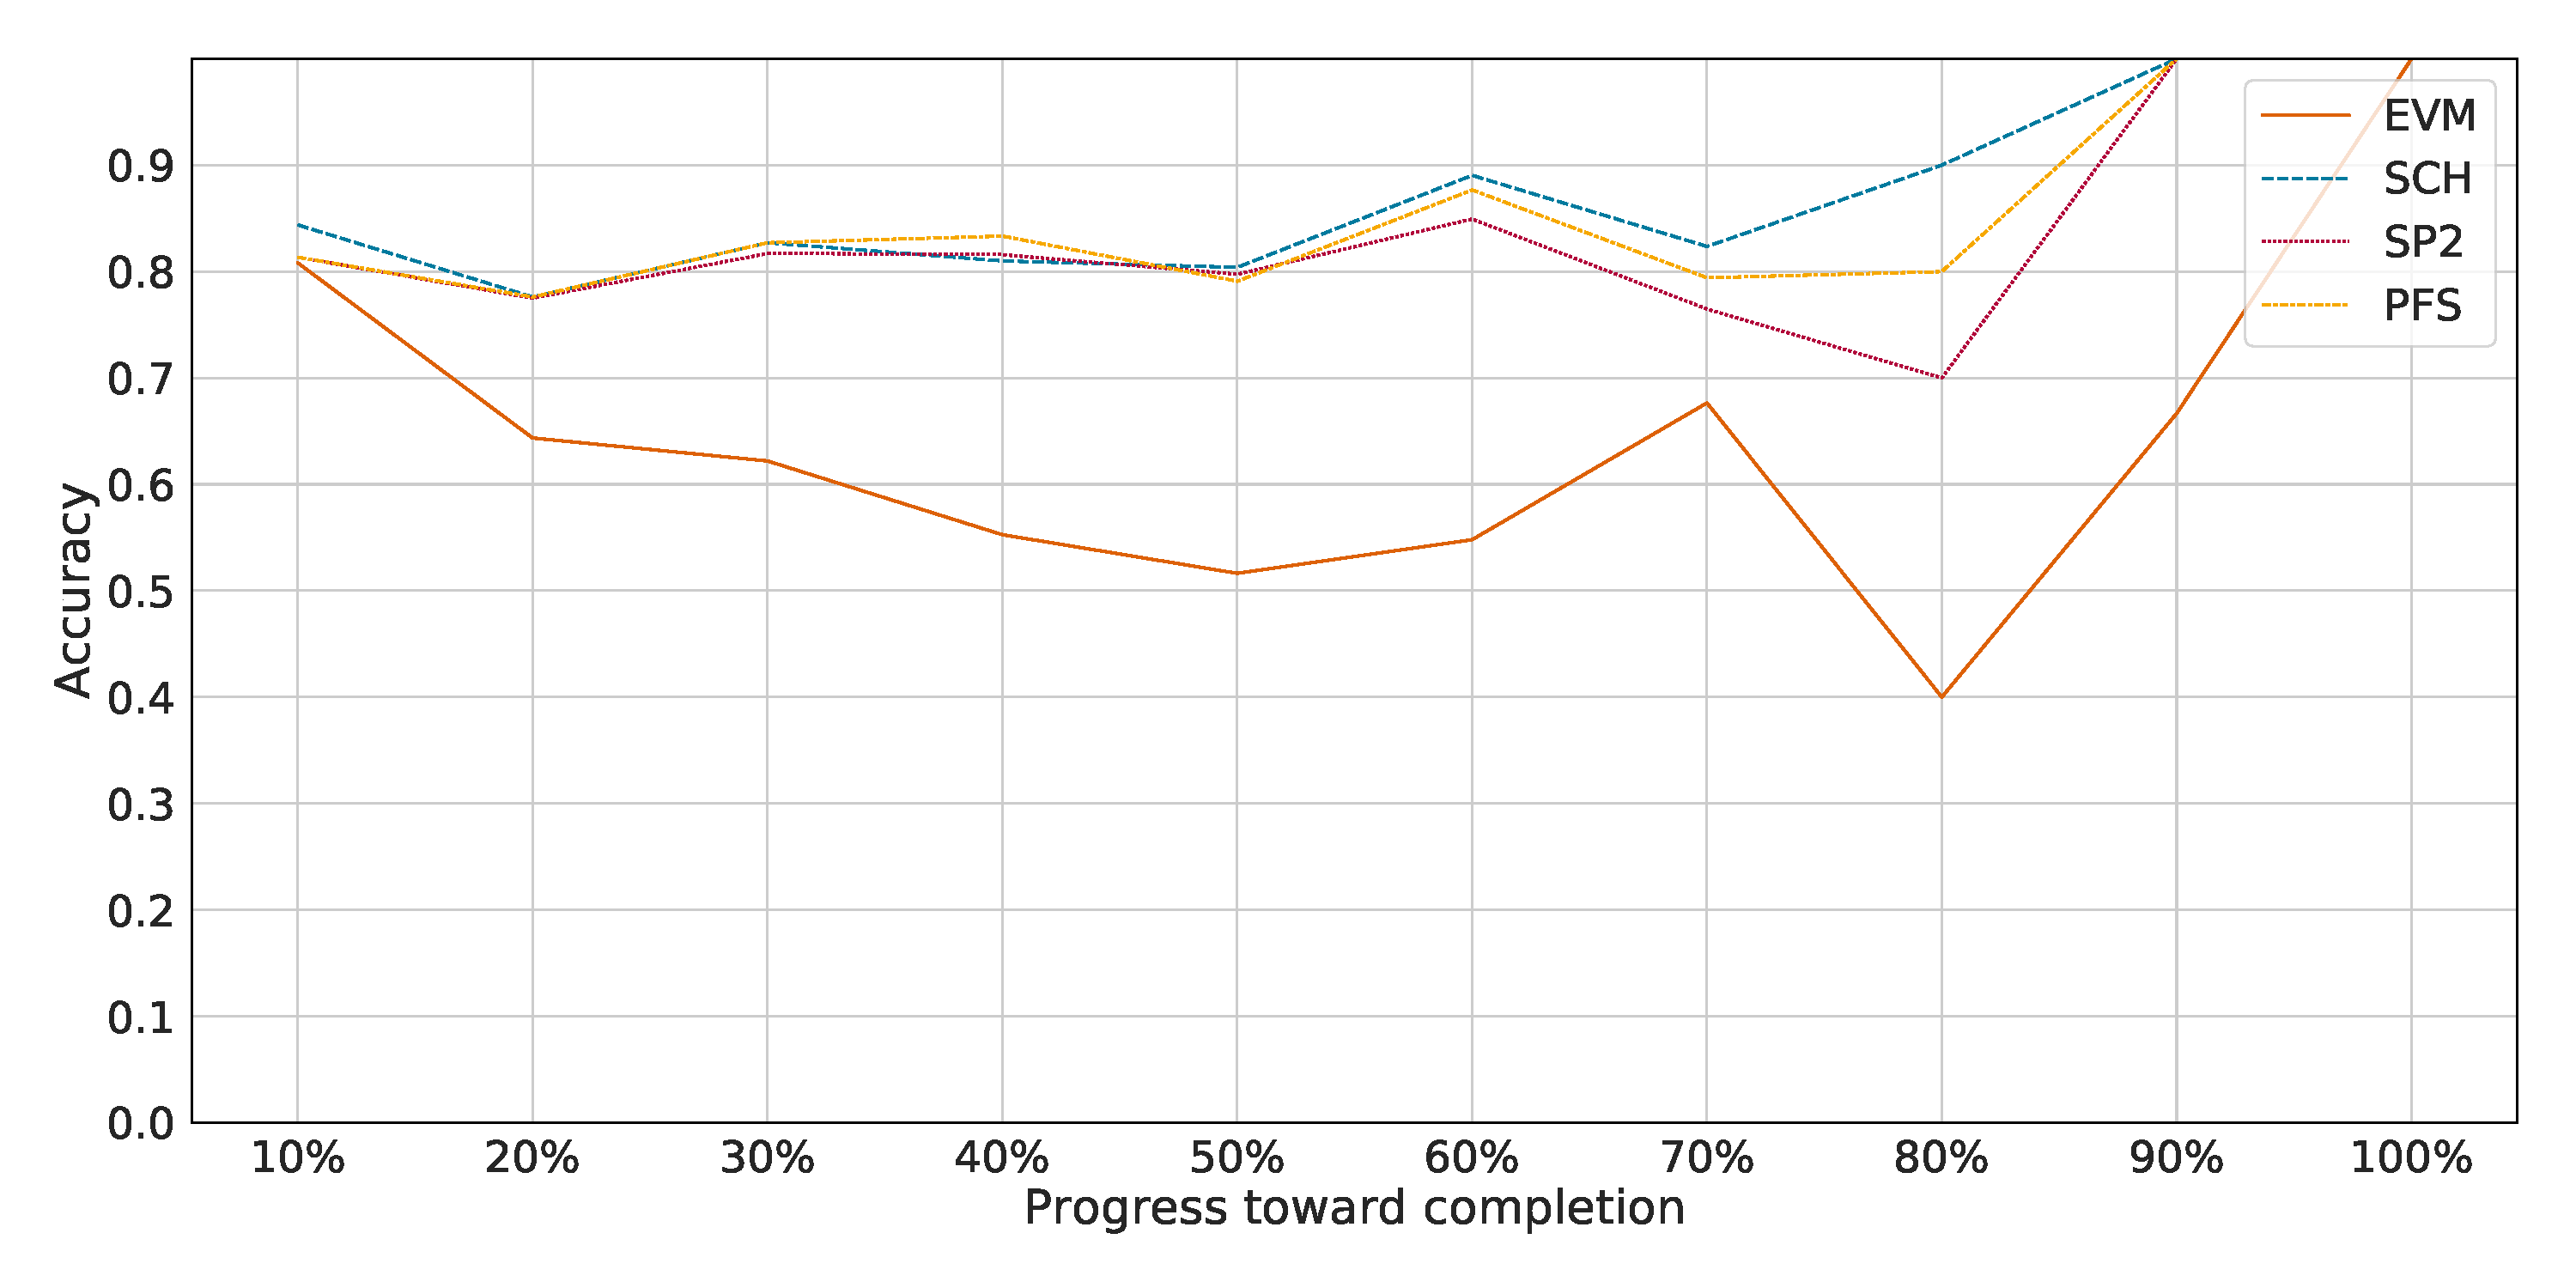
\includegraphics[width=\textwidth]{gfx/helpdesk/individual_stability.pdf}
    \caption{Model stability, individual strategy, HelpDesk}
    \label{fig:helpdesk-individual-stability}
\end{figure}

\paragraph{Stability on BPIC12}
The stability of the predictions on the BPIC12 log is discussed in this paragraph.
\autoref{fig:bpic12-individual-stability} shows the stability of each model with the individual strategy on BPIC12.
The four curves start around $0.8$ and immediately drop by $0.2$.
The EVM curve does not recover from the drop, constantly stays around $0.4$, and finishes around $0.1$.
The other three curves rise back up to $0.9$ at $35\%$ progress.
Then, all three slowly sink toward $0.7$ at $85\%$ and rise sharply toward $1$ at the end.

\autoref{fig:bpic12-grouped-stability} shows the stability of the grouping strategy.
The trajectories of all four curves are mostly as described for the individual strategy.
A small, but notable difference is that the curves of the SCH, SP2 and PFS models are much closer together, and indicate nearly the same values.

In \autoref{fig:bpic12-padded-stability}, the stability for the padding strategy is shown.
The curve trajectories are again very similar to the two aforementioned stability plots, but the overall accuracies are lower.
The EVM model now starts at $0$ accuracy, shortly reaches $0.3$ around $25\%$ and then tapers off back into $0$ accuracy at the end.
The other three curves show a stronger depression around the $75\%$ mark, dropping down to an accuracy of $0.5$, before recovering to $1$ at the end.

Finally, the stability plot of the windowing strategy in \autoref{fig:bpic12-windowed-stability} reveals entirely new curve trajectories.
The EVM curve starts again at $0$, slowly rises to $0.3$, and then edges back down to $0$ in the end.
The SP2 curve starts at $0.8$, drops by $0.1$, and recovers back to $0.9$ until $50\%$ progress.
At this point, there is a sharp decline to $0.7$.
The curve recovers just as sharply, and slowly degrades to $0.6$, and shoots up to $1$ in the end.
The SCH and PFS curves show a similar trajectory as the SP2 curve, albeit less accurate by around $0.150$.

\begin{figure}[!htb]
    \centering
    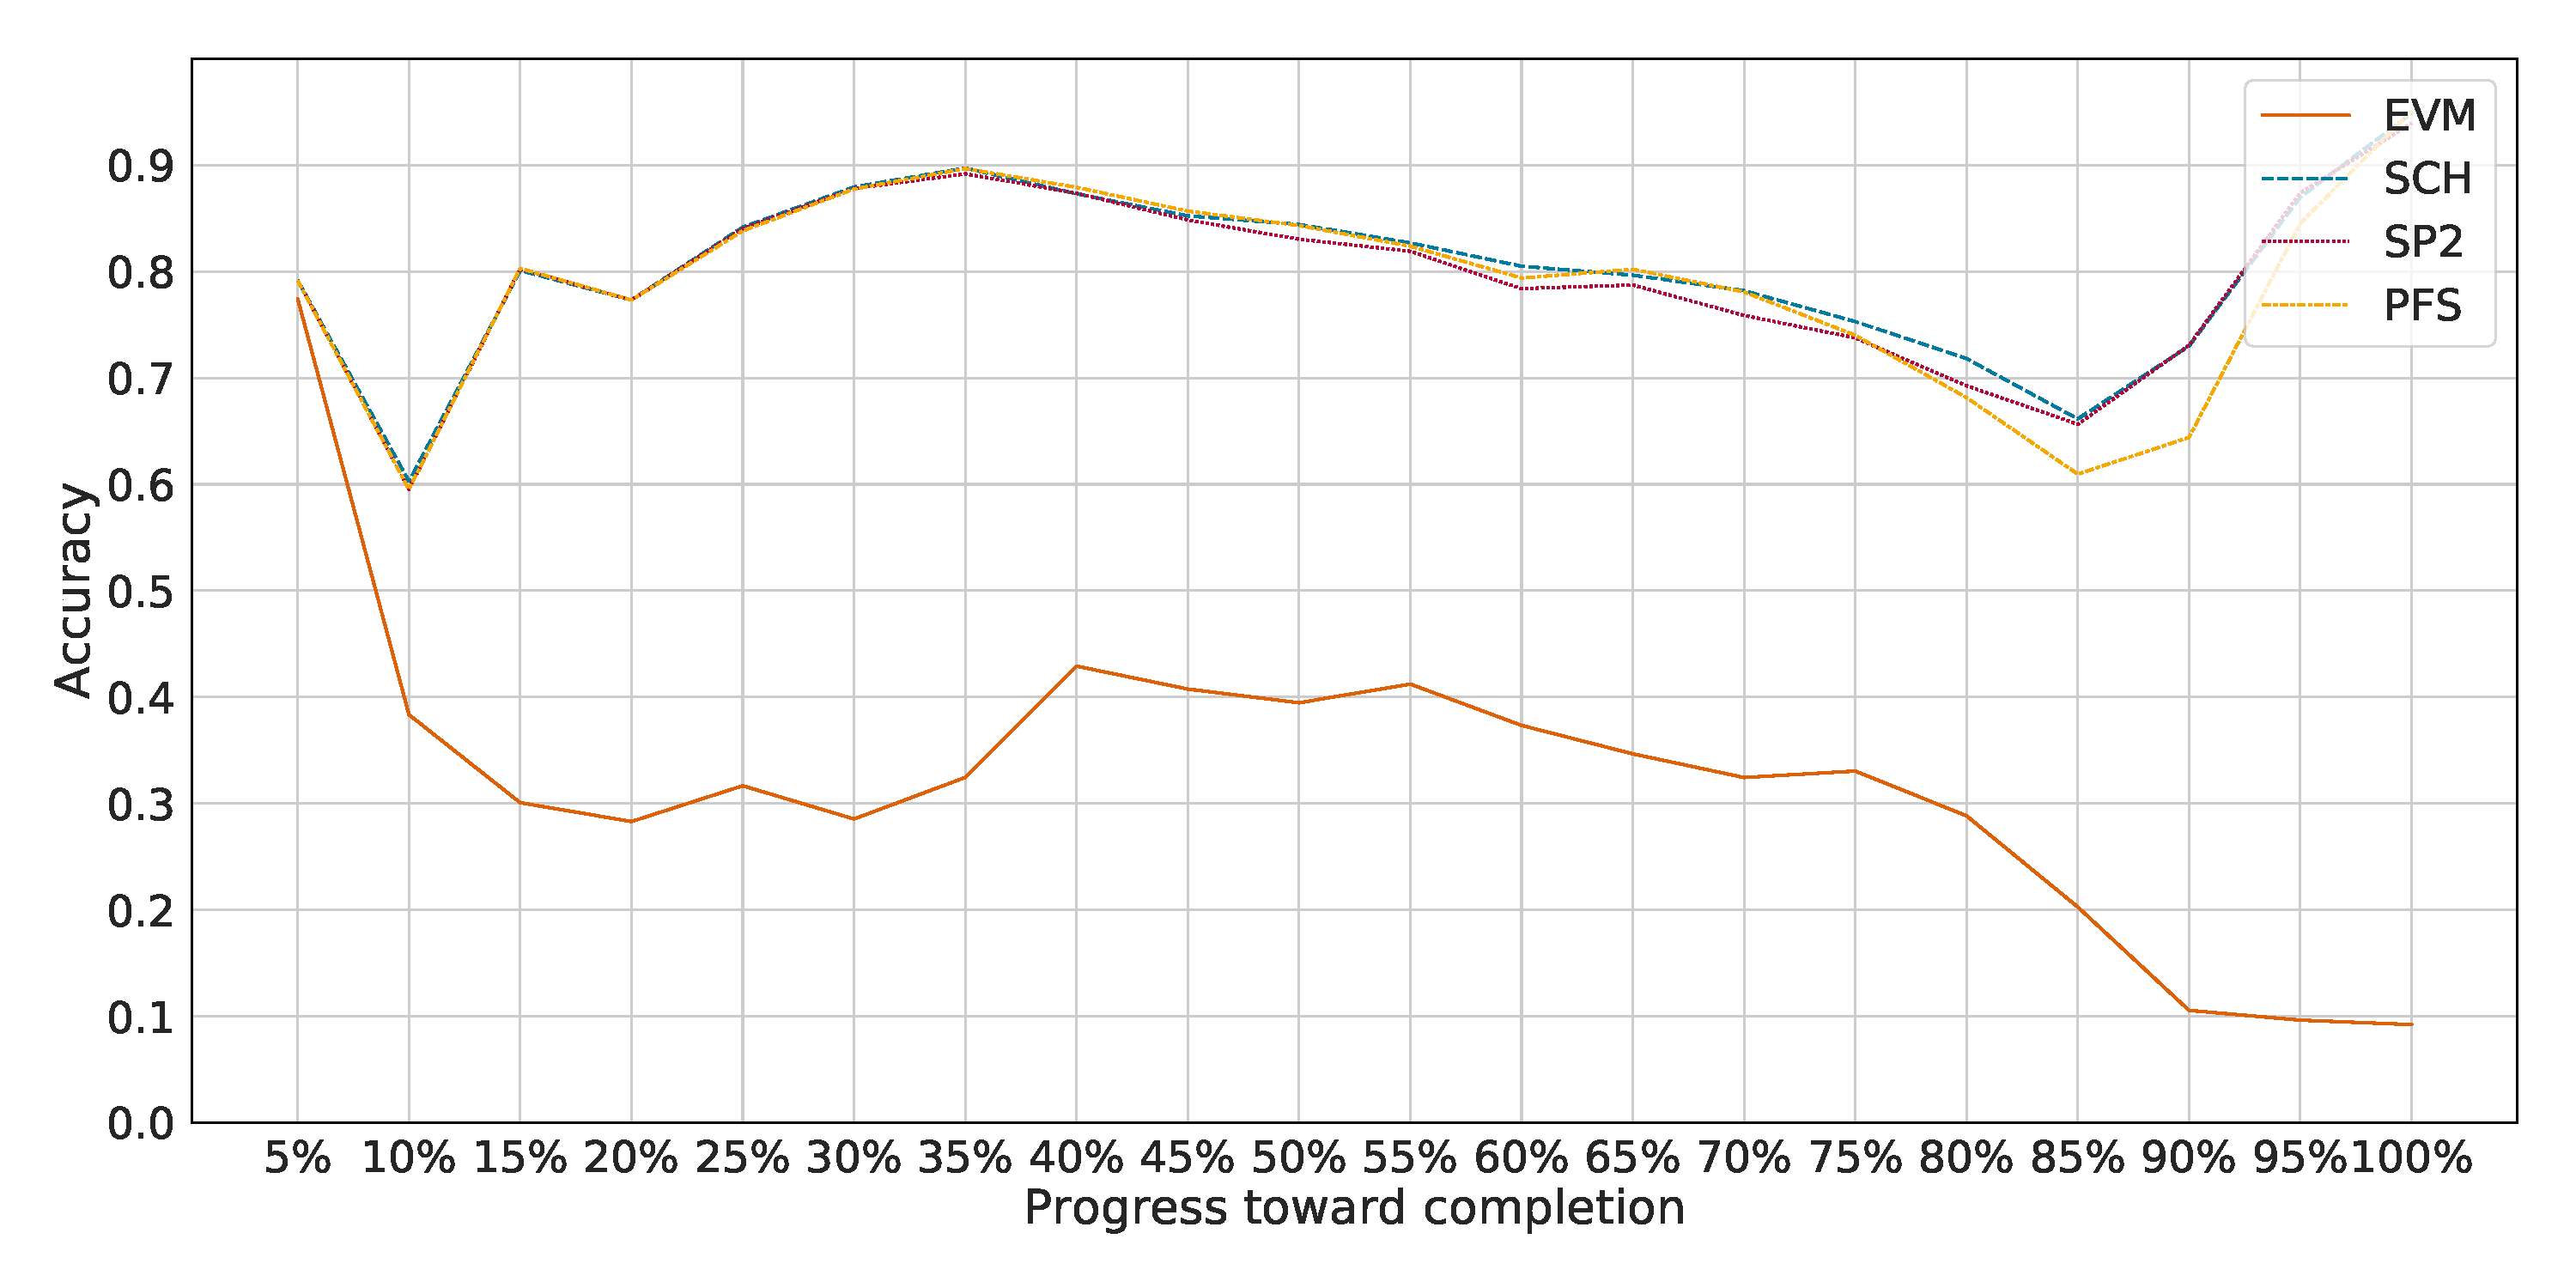
\includegraphics[width=\textwidth]{gfx/bpic2012/individual_stability.pdf}
    \caption{Model stability, individual strategy, BPIC12}
    \label{fig:bpic12-individual-stability}
\end{figure}

\paragraph{Stability on BPIC15}
The BPIC15 log with its five datasets is discussed in this paragraph.
The figures \autoref{fig:bpic15-5-individual-stability} and \autoref{fig:bpic15-5-grouped-stability} show the stabilities for the individual and grouping strategies on BPIC15-5.
In the appendix, \autoref{fig:bpic15-1-individual-stability} to \autoref{fig:bpic15-5-windowed-stability} illustrate the remaining curves for the remainder of the log.
The curves across BPIC15-1 to BPIC15-5 are very similar within a specific strategy, which is why we give a general description of the observations for each strategy in the following.

In the stability plot of the individual strategy in \autoref{fig:bpic15-5-individual-stability}, the EVM curve shows a very low accuracy.
Similar to the two logs before, the curve starts with a steep decline from $0.5$ to $0.1$ and then stays around this accuracy. In the end, the curve shoots up to $0.35$.
The SCH, SP2 and PFS curves all start at $0.7$ and slowly sink to around $0.5$ at $80\%$.
Then, all three curves see an increase of $0.2$, with the SP2 curve ending at $0.75$.
The SCH curve ends at $0.7$, and the PFS curve at $0.6$.

The stability plot for the grouping strategy in \autoref{fig:bpic15-5-grouped-stability} shows very similar curve trajectories.
In contrast to the individual strategy, the SCH, SP2 and PFS curves are a lot closer together, and the PFS model does not see as sharp a drop.
This is a theme that is visible on the other BPIC15 datasets, too.

The stability plots for the padding strategy show steadily declining curves for SCH, SP2 and PFS models from $0.7$ at the beginning towards an accuracy of $0.4$ around $90\%$ progress.
Then, the curves jump up by $0.2$ to $0.3$ to finish around $0.7$.
The EVM curve barely surfaces above $0$.
For BPIC15-1 and BPIC15-4, the SCH curve also dips down after the start.
On BPIC15-1, the PFS curve also dips down, leaving the SP2 curve as the sole remainder on the steadily declining trajectory previously described.

The plots for the windowing strategy show a simple picture.
The EVM curve is stuck at 0.
The SCH and PFS curves start around $0.6$, and descend toward $0.3$, spiking up toward $0.5$ at the end.
The SP2 curve hovers above, starting around $0.7$, and linearly descends to $0.5$ until $90\%$ progress.
Then, it also jumps up by $0.3$ at the end of the plot.

\begin{figure}[!htb]
    \centering
    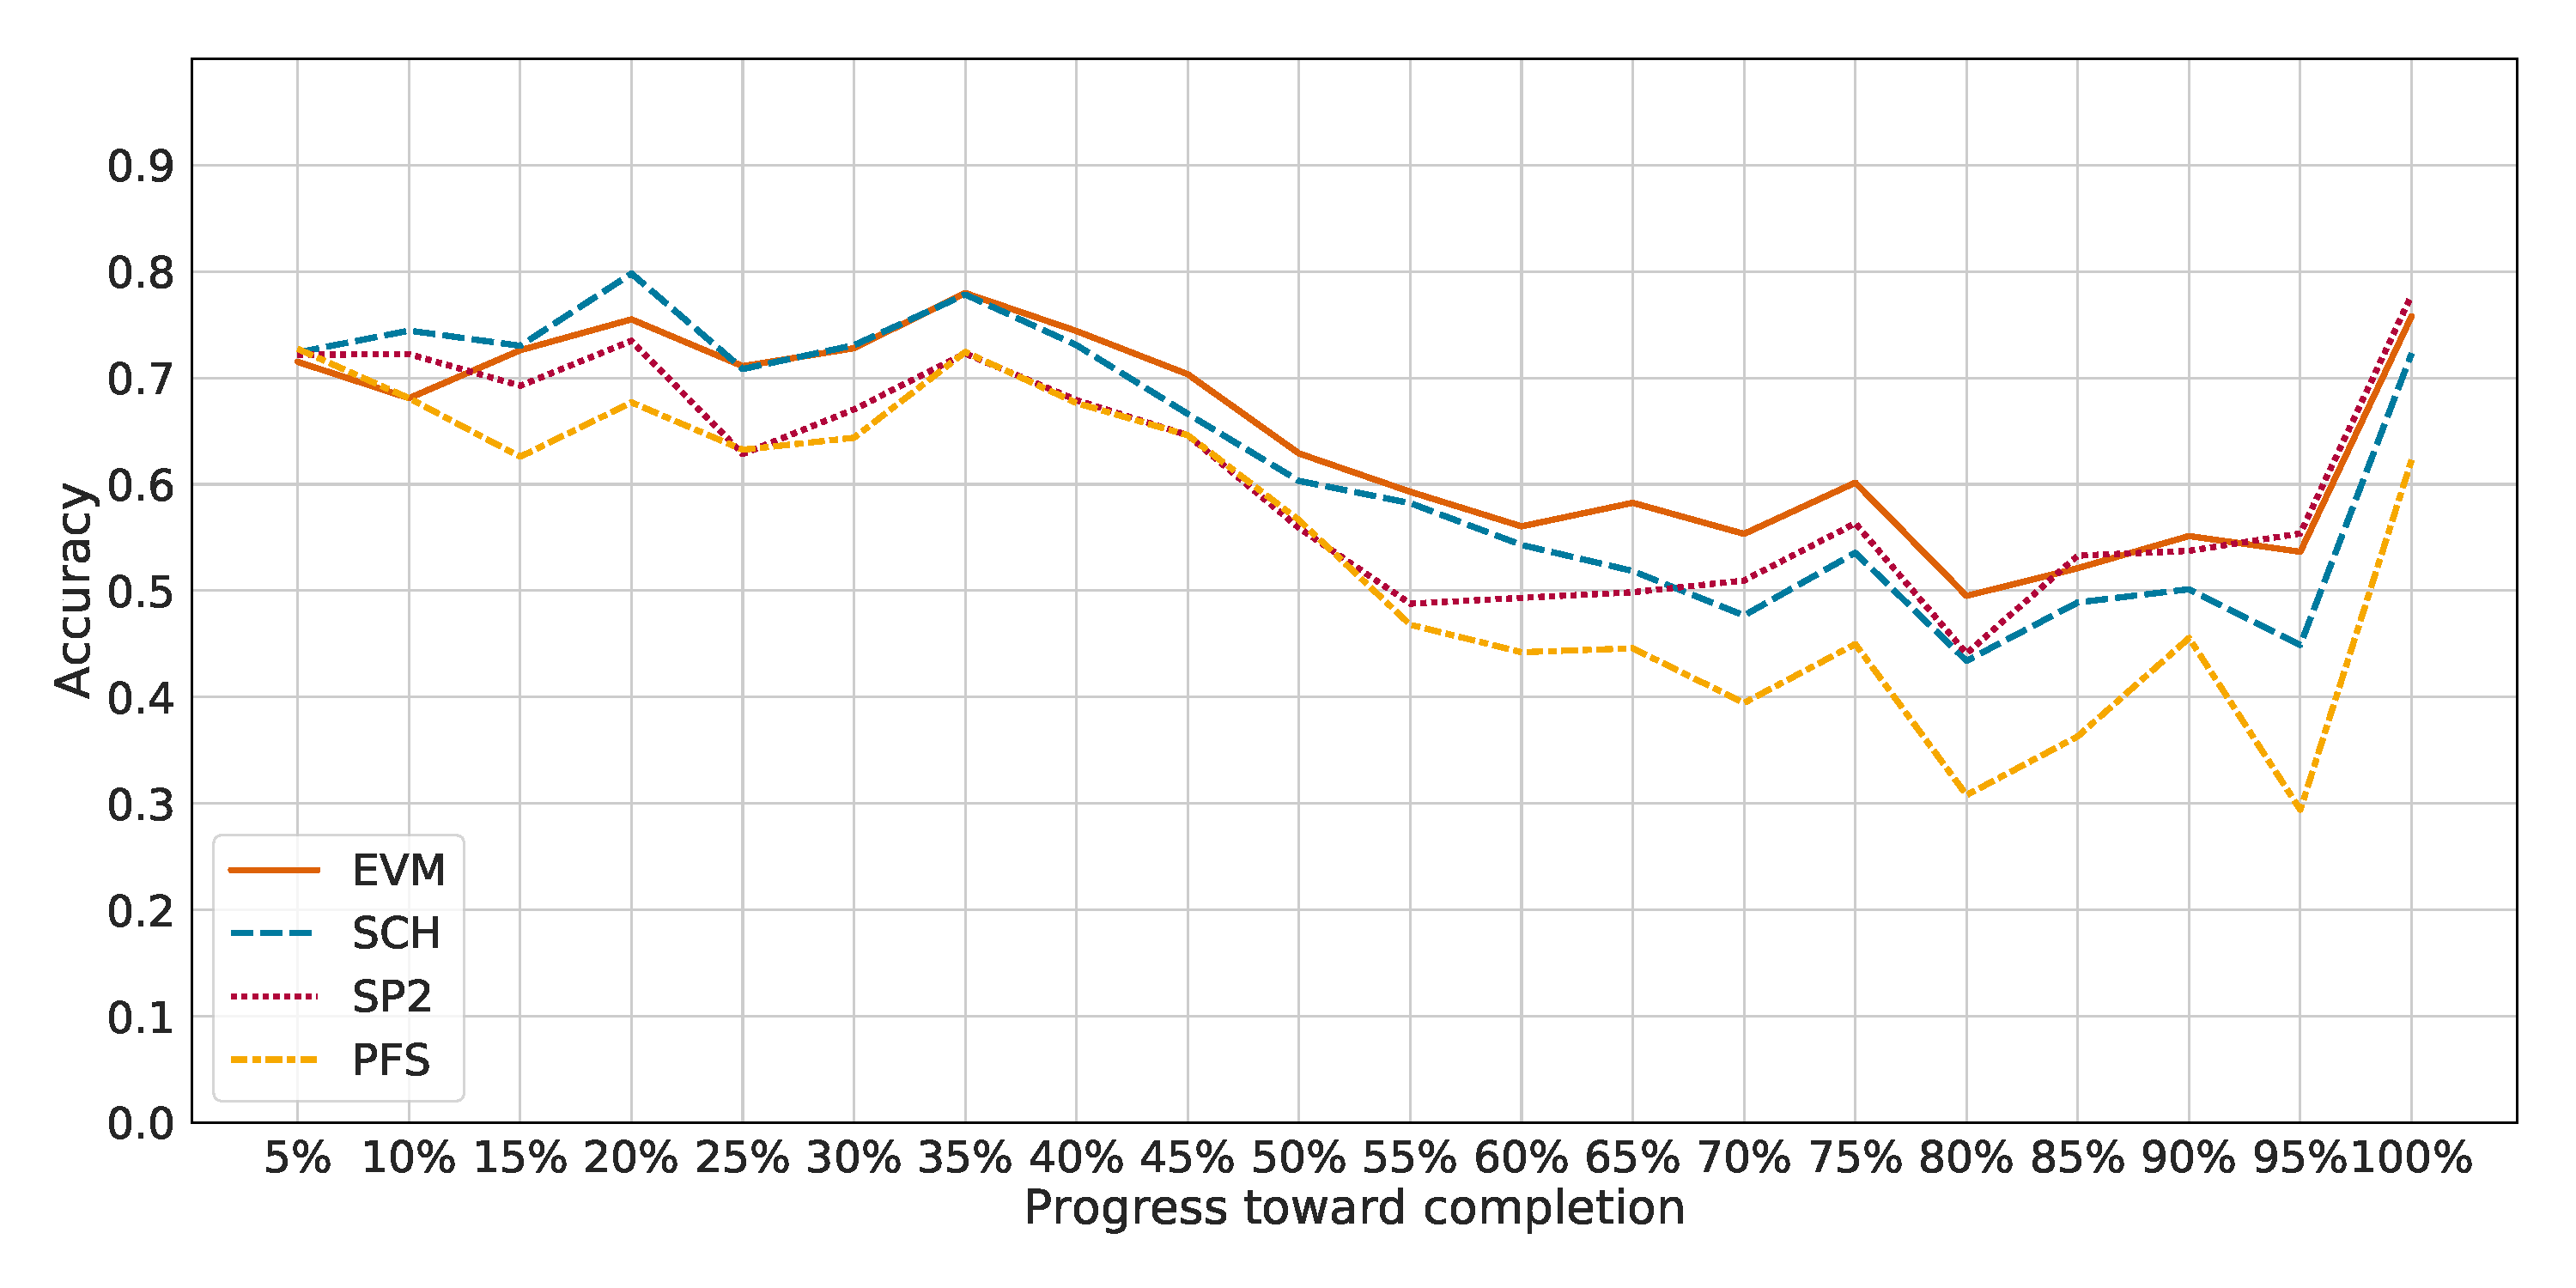
\includegraphics[width=\textwidth]{gfx/bpic2015_5/individual_stability.pdf}
    \caption{Model stability, individual strategy, BPIC15-5}
    \label{fig:bpic15-5-individual-stability}
\end{figure}
\begin{figure}[!htb]
    \centering
    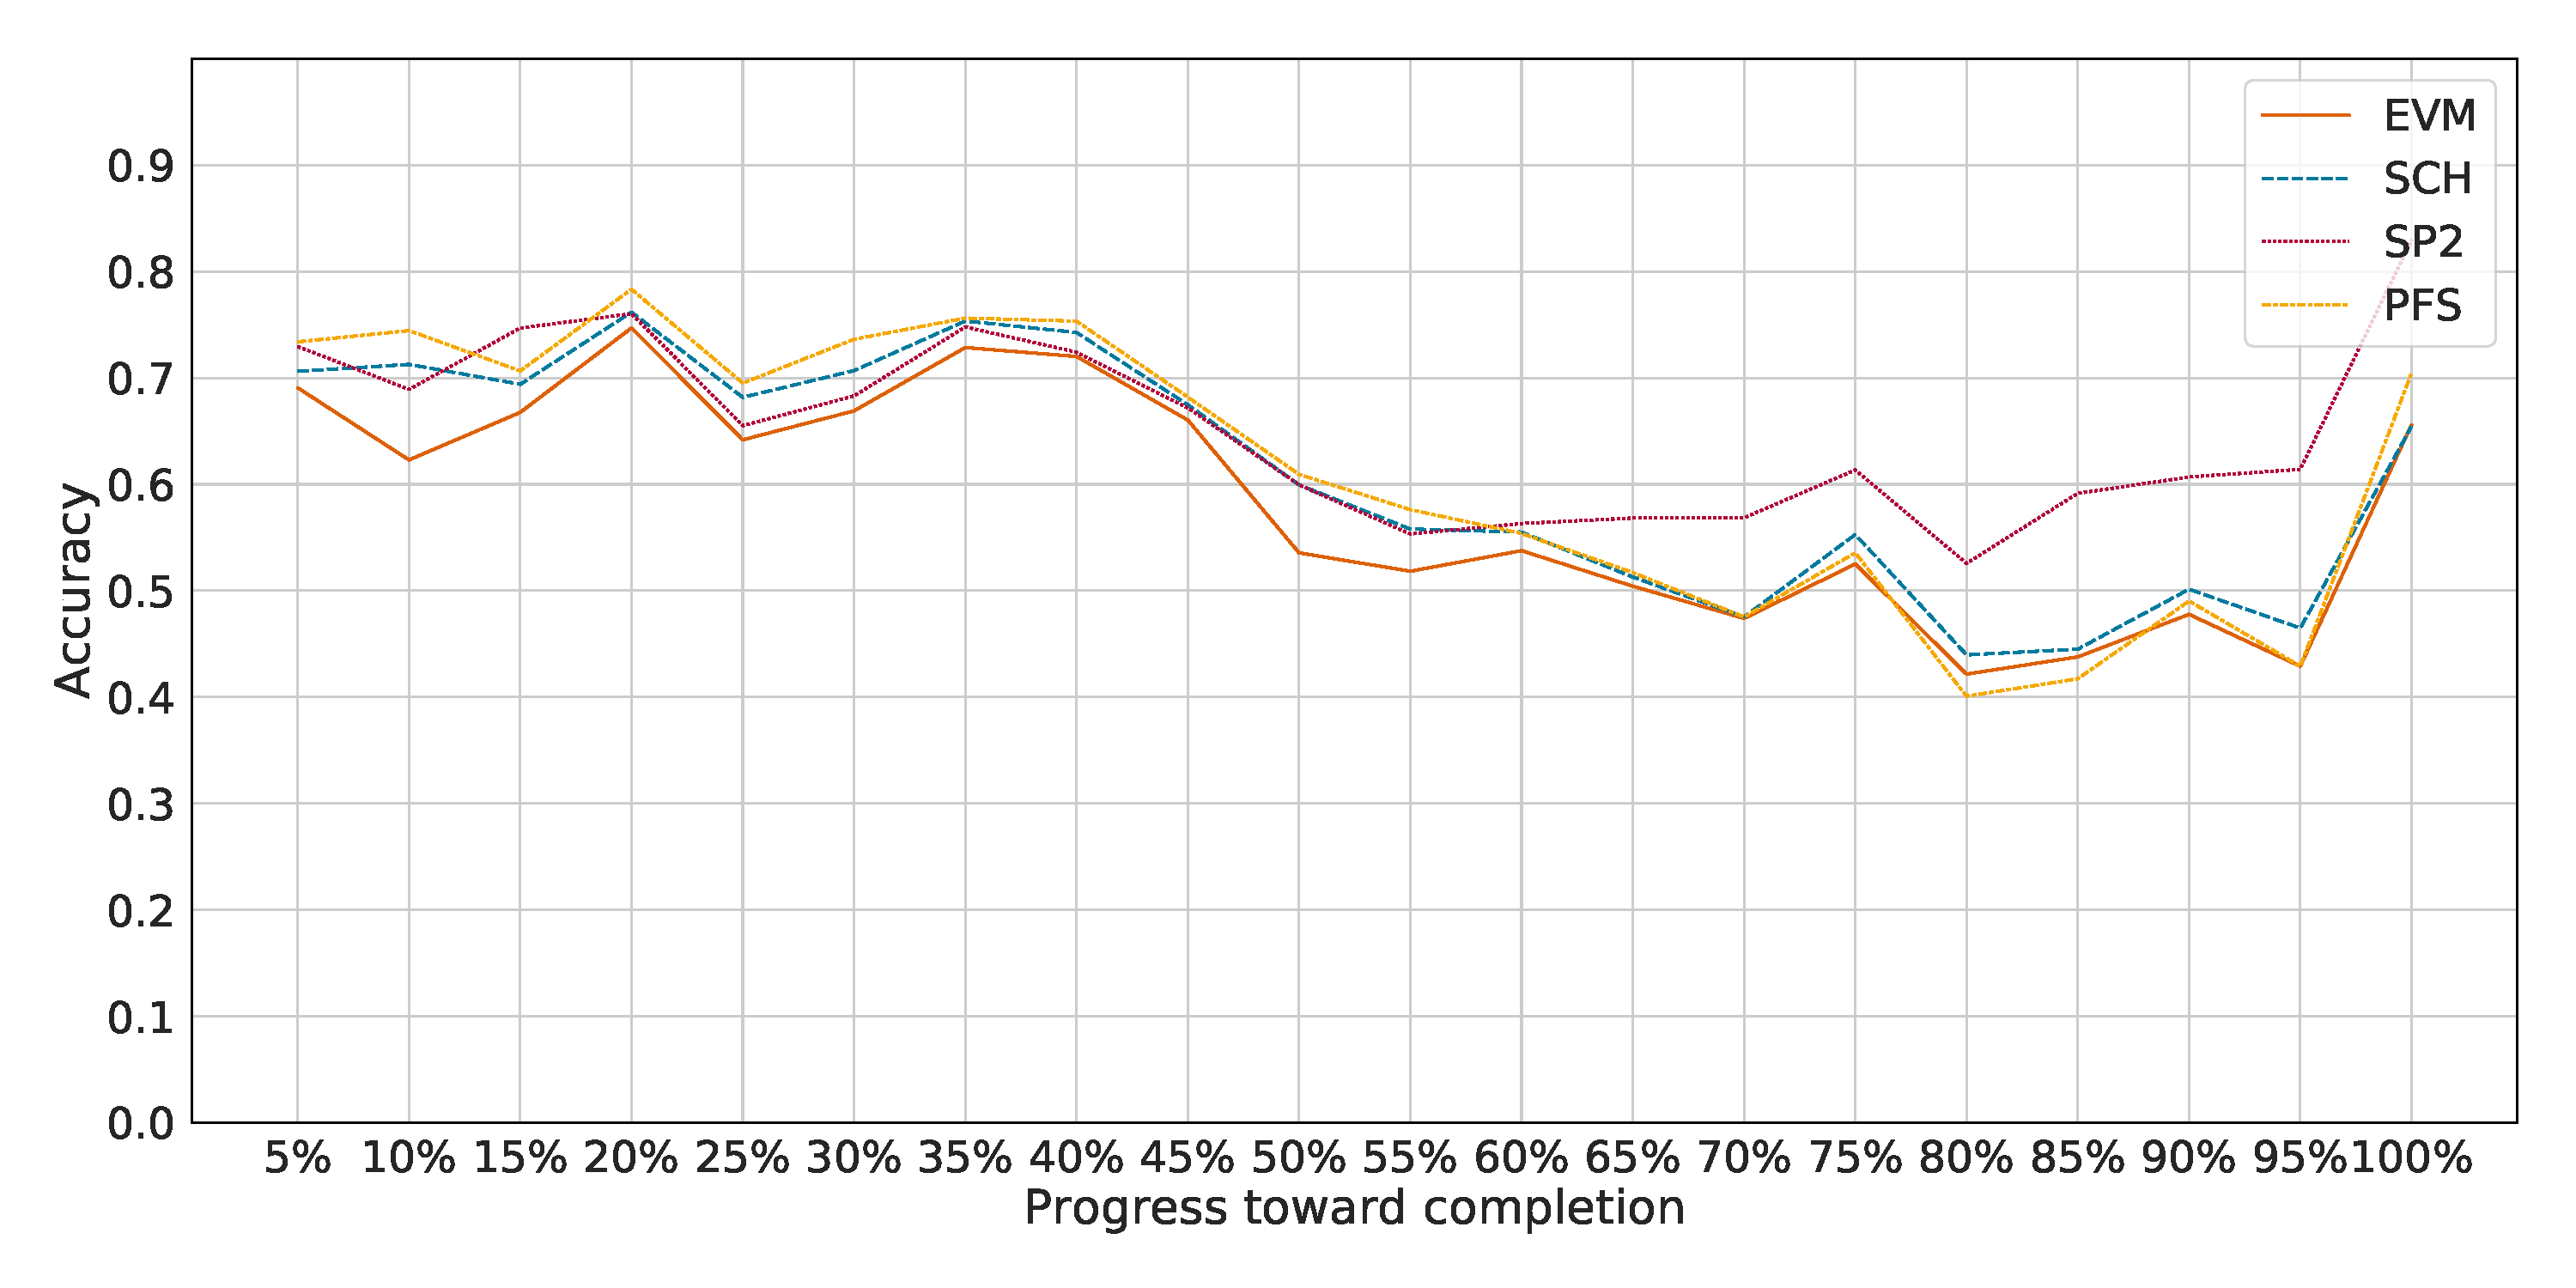
\includegraphics[width=\textwidth]{gfx/bpic2015_5/grouped_stability.pdf}
    \caption{Model stability, grouping strategy, BPIC15-5}
    \label{fig:bpic15-5-grouped-stability}
\end{figure}
\newpage
\paragraph{Stability on BPIC11}
This paragraph covers accuracy stability on the BPIC11 log.
The most informative plot for this dataset is shown in \autoref{fig:bpic11-grouped-stability} for the grouping strategy.
It illustrates how the accuracy is relatively constant for the SCH, SP2 and PFS models around $0.7$.
It does not drop in the beginning, nor does it spike at the end of the process.
Also, the plot illustrates well how close the curves of the three models are.
The EVM model stays constant at around $0.10$ accuracy.

Little do the curves change for the individual strategy.
Only two minor differences surface: The SCH and PFS curves are further apart, and the SP2 curve drops asymptotically from $0.65$ in the beginning to $0.1$ at the end.

With the padding strategy, the SCH, SP2 and PFS curves start around $0.75$, drop to approximately $0.55$ and stay constant until the end of the process.
The EVM curve starts at $0$ and slowly grows until $0.1$ at the end.

The windowing strategy makes the drop of the SCH, SP2 and PFS curves more pronounced from $0.75$ in the beginning to just above $0.4$ from $35\%$ onwards.
From there on, the curves stay constant.
The EVM curve constantly hovers at $0.1$.

\begin{figure}[!htb]
    \centering
    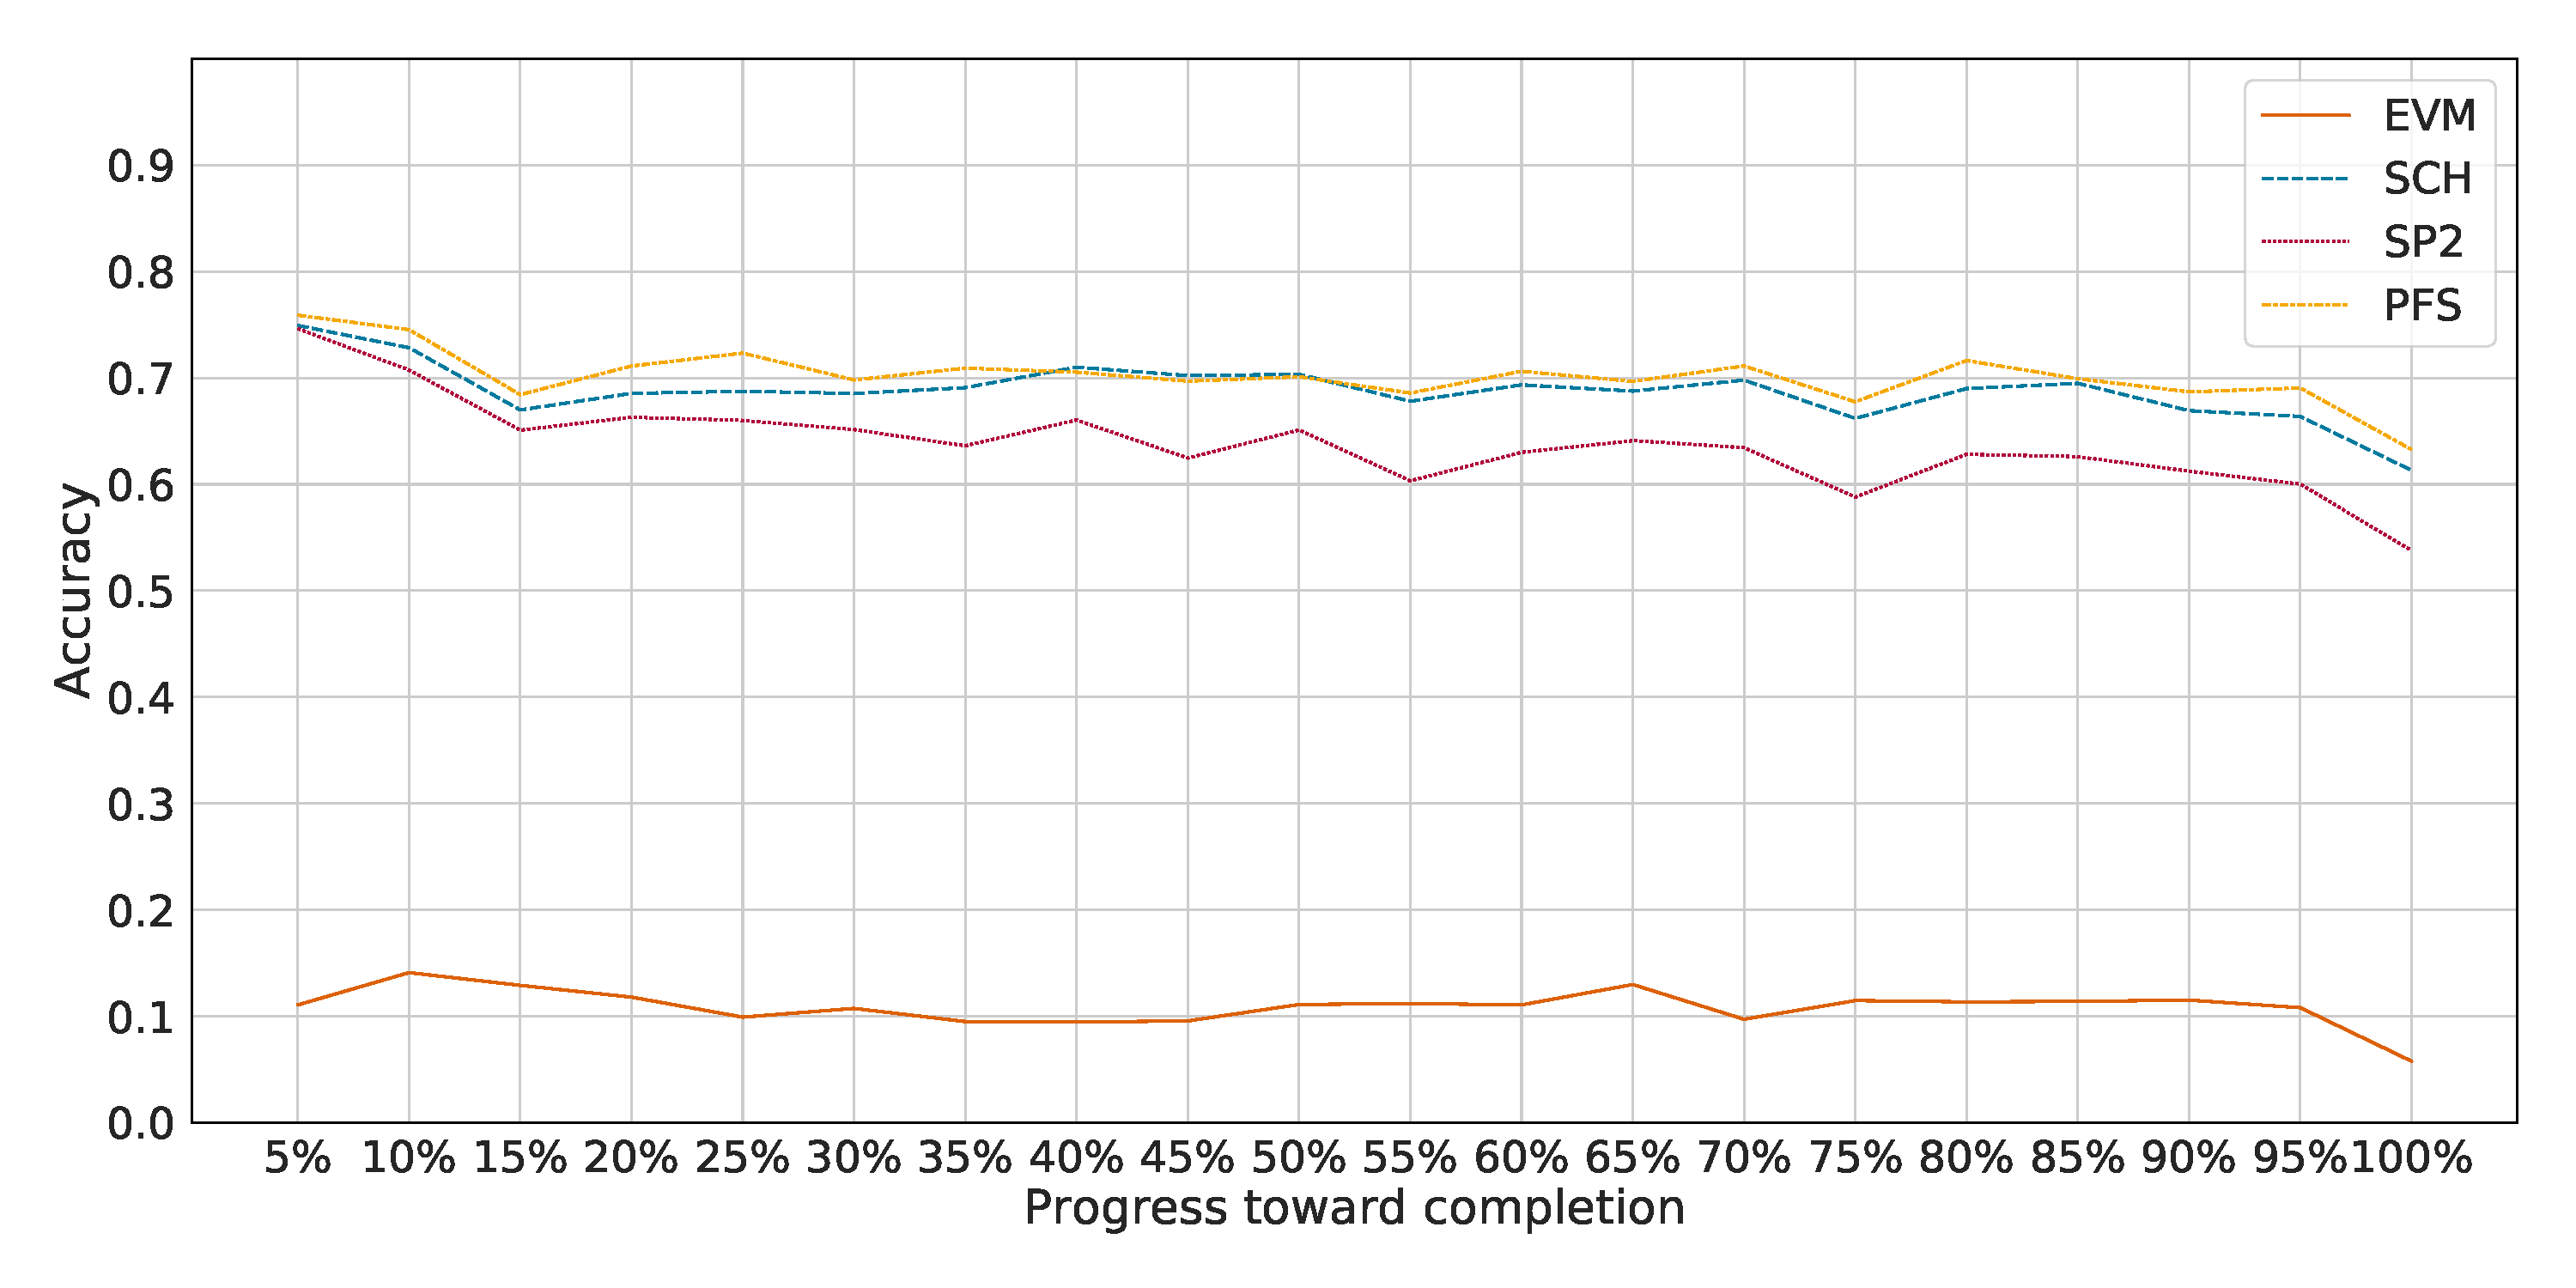
\includegraphics[width=\textwidth]{gfx/bpic2011/grouped_stability.pdf}
    \caption{Stability curves for grouping strategy on BPIC11}
    \label{fig:bpic11-grouped-stability}
\end{figure}

\paragraph{Verdict on stability}
In our verdict on the stability measurements across all datasets, we focus on five key observations.

First, we observed that many accuracy curves started with a drop in accuracy.
Similarly, accuracy spiked up towards the end of the process, like on the BPIC12 log.
The BPIC12 log contains traces from a process that covers a loan application.
On this log, the accuracies taper off until $85\%$ progress, when they spike up again.

\begin{figure}[!htb]
    \centering
    \begin{adjustbox}{center}
    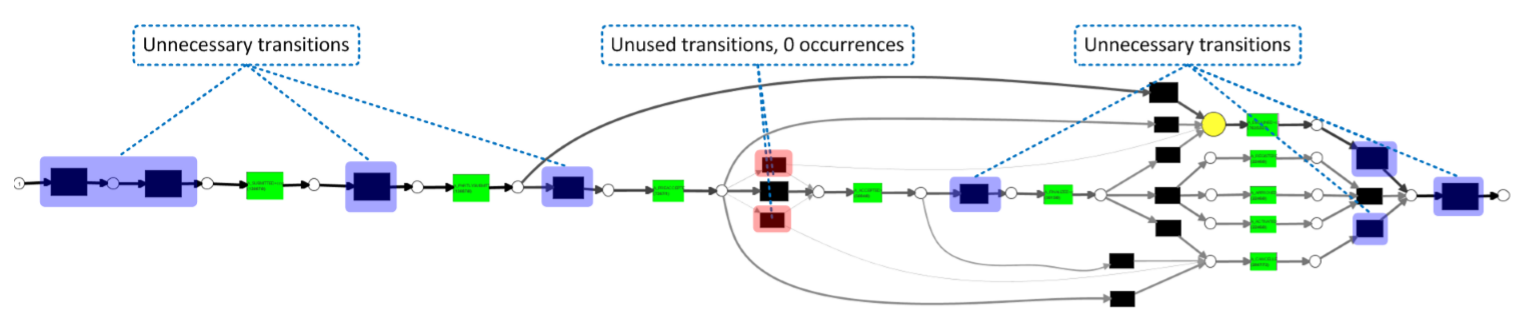
\includegraphics[width=1.25\textwidth]{gfx/bpic12-mined-process.png}
    \end{adjustbox}
    \caption[A mined process model from BPIC12]{A mined process model from BPIC12. Illustration taken from~\cite{adriansyah2012mining}}
    \label{fig:bpic12-mined-process}
\end{figure}

\autoref{fig:bpic12-mined-process} reveals a process model that was mined from BPIC12 in \cite{adriansyah2012mining}.
Seeing the model in context with the stability curve reveals that the accuracy drops and spikes could be related to the varying degrees of complexity in different stages of the process.
Every application begins in the same way, i.e. variability in the first stages of the process is low, which might cause accuracy to be high.
As the process progresses, the variability becomes higher, which correlates with the accuracy decline until $80\%$ progress.
The processes in BPIC12 always end either on approval or dismissal of the application, boosting accuracy from the moment that no more splits have to be anticipated.
This could hint at a connection between prediction accuracy and complexity of the stage of a process.

Second, we realized that the grouping strategy did not only contribute to high overall results but brought curves closer together for the SCH, SP2 and PFS models.
This might be a symptom of a harmonizing effect of the strategy.
We visualized this effect in \autoref{fig:grouping-accuracy-harmonization}.
The heatmap shows the standard deviation among the best accuracies of the SCH, SP2 and PFS models for each dataset and strategy.
It is clear that the grouping strategy leads to the lowest standard deviations.

\begin{figure}
    \centering
    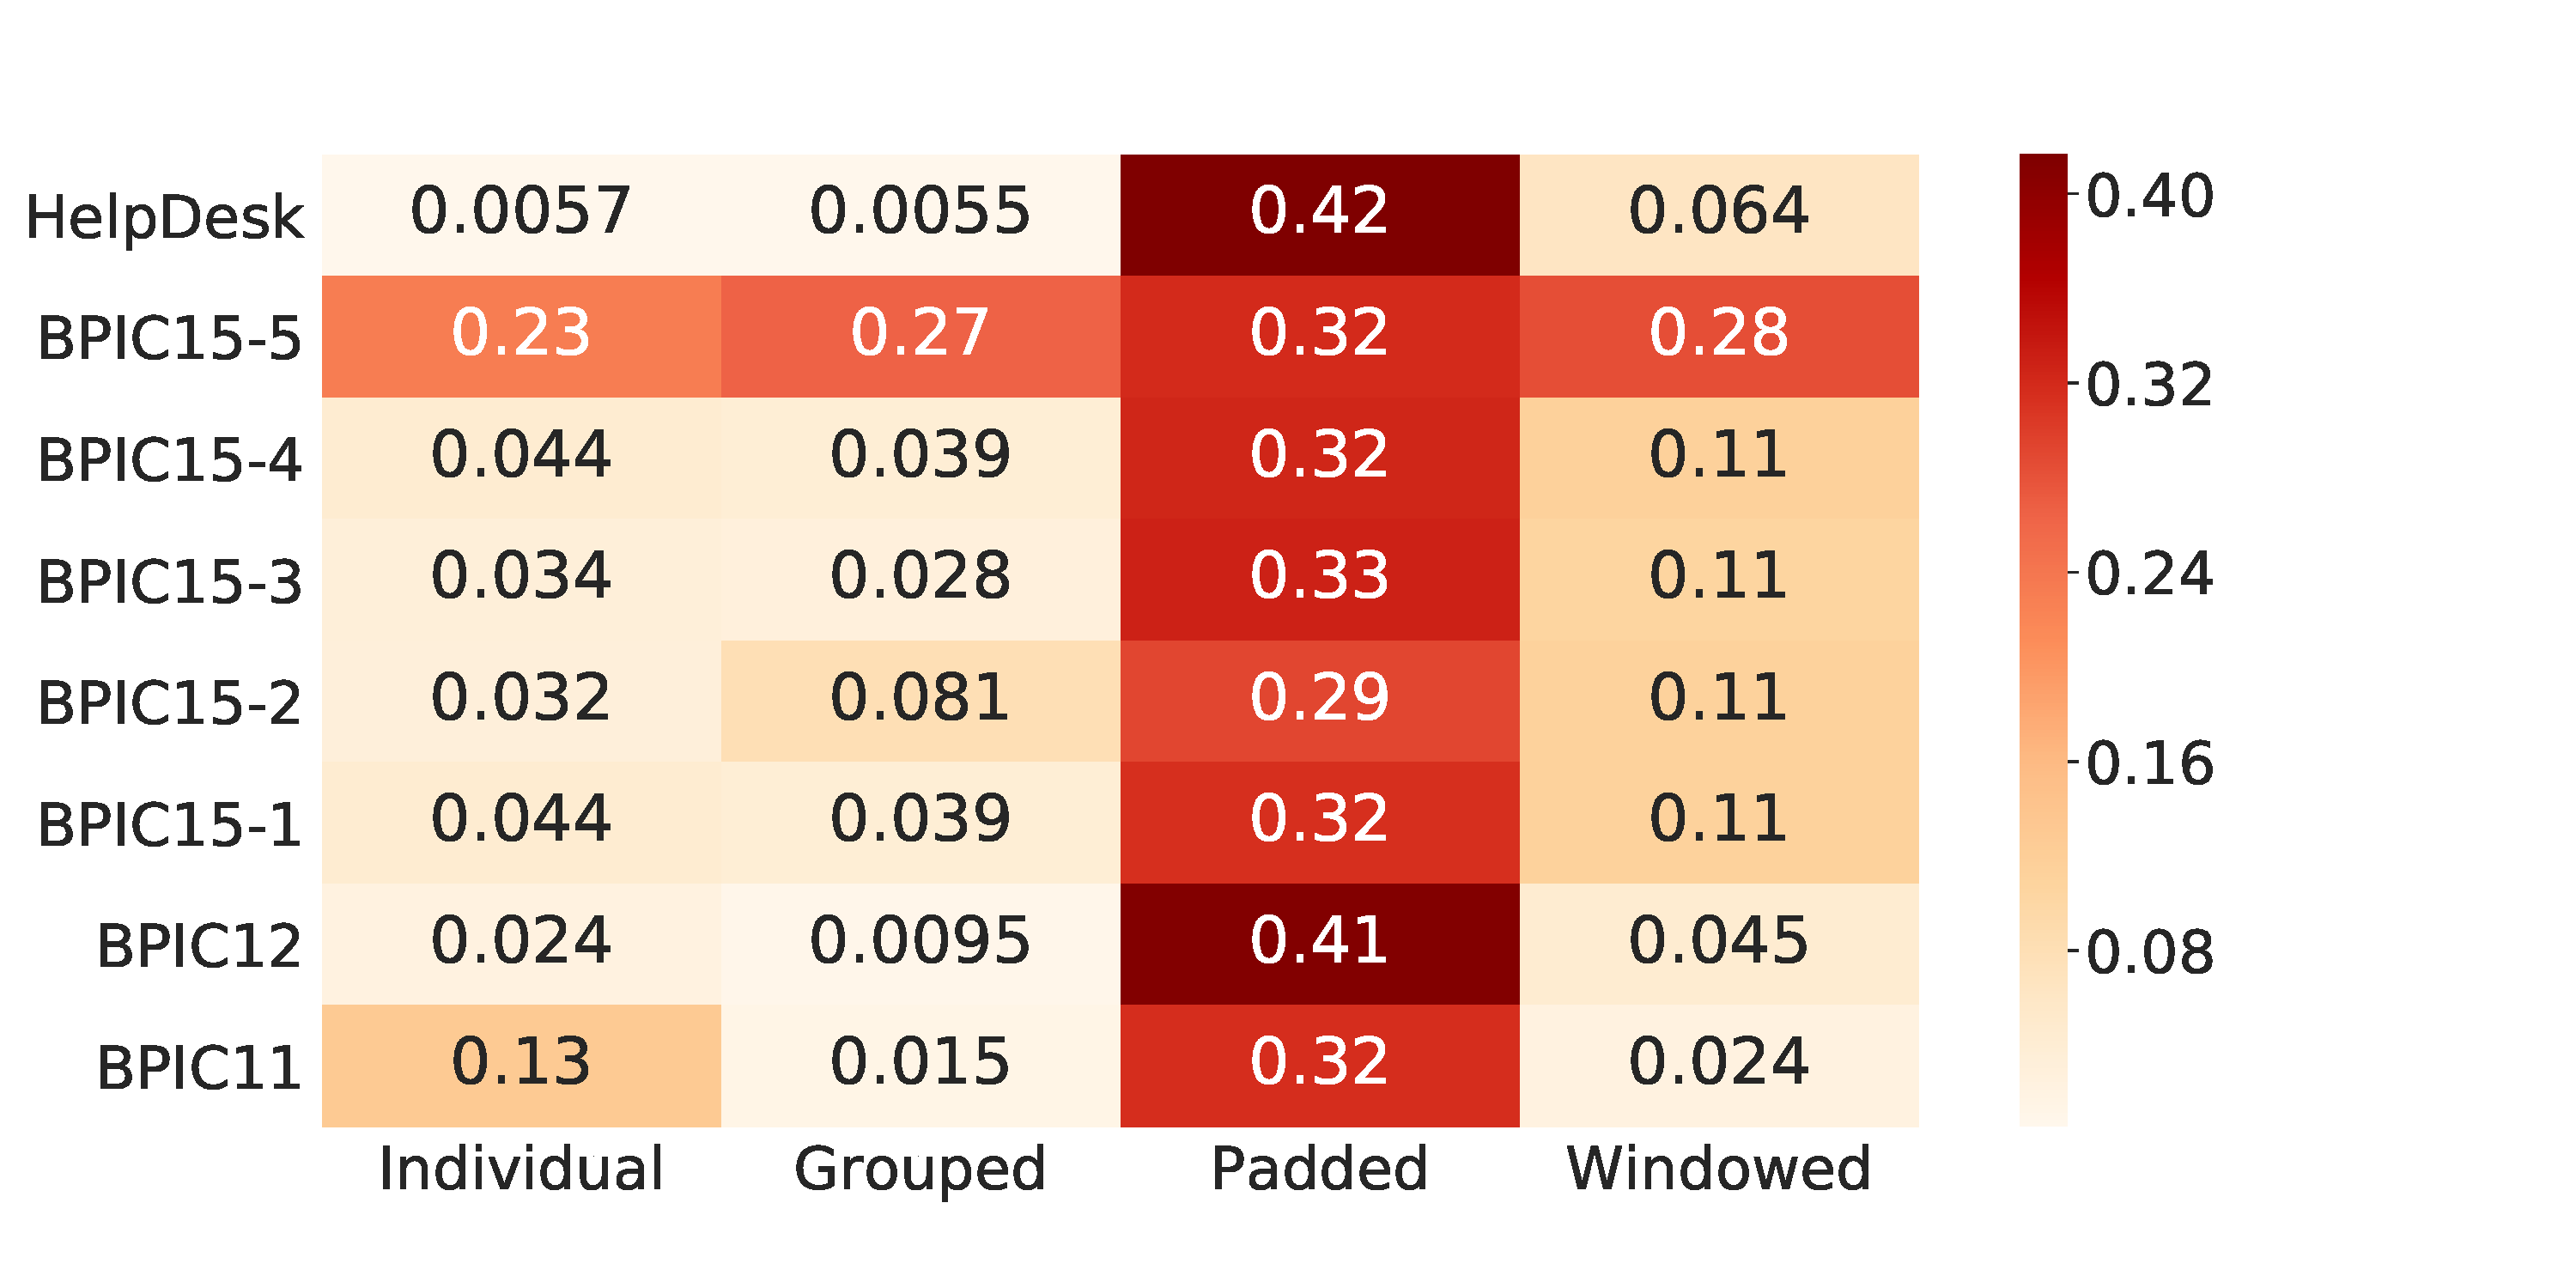
\includegraphics[width=\textwidth]{gfx/grouping-accuracy-harmonization.pdf}
    \caption[Batching strategy harmonizes top accuracies]{The grouping strategy often reduces the standard deviation between the highest accuracies of SCH, SP2 and PFS models}
    \label{fig:grouping-accuracy-harmonization}
\end{figure}

Third, the SCH, SP2 and PFS models all produce similar accuracy curves.
The EVM curves are different in that they are not only deficient, they also do not show the same corrections.

Fourth, the windowing strategy incurs very unstable curves.
While this statement seems to be especially true for the longer processes in BPIC11 and BPIC15, the windowing strategy seems to have less of an impact with shorter processes as evidenced with BPIC12.

Fifth, the SP2 model best handles the missing history on the windowing strategy.
Its curves are the highest among the windowing strategy measurements on any dataset.
Also, the SP2 accuracy curves on the windowing strategy are among those with the smallest fluctuations.\\

We will connect these observations to the other findings from the other verdicts in the following section.

\section{Discussion}\label{sec:eval:discussion}
In this section, we connect the observations made in the previous sections on accuracy, timing, and stability of the models.
Furthermore, we discuss resulting learnings and potential reasons.\\

The EVM model consistently underperforms, although it trains faster.
Furthermore, it has phases in some processes during which it delivers $0$ accuracy.
The SCH model works a lot better, although both architectures are very similar.
Indicated by the barely converging loss curves in \autoref{appendix:loss-curves}, there is reason to believe that something prevents the EVM model from improving.
The fundamental difference between the EVM and SCH models is an embedding layer, which we suspect to be the cause for the low accuracy.
We believe that the embedding layer requires more datapoints per target class than currently included to perform well.
In the HelpDesk log, there is a tiny number of classes and a large number of traces, which could be a reason for the EVM model scoring above $0.720$.
The faster training speed can be attributed to the use of the SGD optimizer, which is commonly known to produce the fastest convergence.
Another reason for the big difference between our accuracies and those of Evermann et al. could be the implementation.
\todo[inline]{cite here, do you know a source haojin?}
The original authors used the low-level Tensorflow framework directly, which could have enabled further optimizations.\\

We find that the grouping strategy frequently delivers the best results in terms of speed and accuracy.
Nonetheless, there is potential for optimization, as the relatively low accuracy on BPIC12 suggests.
The reason for this accuracy can be found in \autoref{tab:dataset-characteristics} and \autoref{tab:batch-sizes}.
BPIC12 has the highest number of traces, and a relatively even distribution of lengths, resulting in a small standard deviation.
This makes the strategy place too many traces into a single batch, causing lost optimization opportunities.
With this in mind, the grouping strategy should be enhanced to split batches if they exceed a certain size threshold.\\

We were also able to confirm Klinkmüller et al. and their statement that the windowing strategy leads to unstable results~\cite{klinkmuller2018reliablemonitoring}.
While it may be a performant strategy to use for time-series prediction, it does not work very well for predicting the future of a single case.\\

Furthermore, we expected the models to become more accurate toward the end of the process.
This did not turn out to be the case, but instead, we saw a connection of process complexity and accuracy.
This connection was visible both in absolute accuracy and in accuracy stability measurements.
\autoref{tab:strategy-top-accuracies} on page \pageref{tab:strategy-top-accuracies} shows that the mean accuracy of the three top-performing models on each dataset goes down as the process complexity goes up.
In the stability measurements, it was possible to see that the models gave very accurate predictions in phases of low variability.
For instance, the BPIC12 and HelpDesk logs cover processes which start with a receiving phase.
The reception of an application or the creation of a ticket always entails the same steps.
For this reason, the accuracy is high in these initial stages.
A similar phenomenon can be seen toward the end of these processes.
An application is either rejected or accepted, and a ticket is always closed.
This simplicity at the end of the process could explain the jumps in accuracy.

It is worth reflecting on this last point.
If a machine learning model is incapable of understanding the choices made in certain phases of a process, it could either be a data problem or a process problem.
In the latter case, a potential reason could be that decisions in phases of low accuracy are not standardized or overly complicated.
Using the stability information in this way could create a feedback loop for process optimization.\\

After discussing potential reasons for our findings and consequences thereof, we compare our accuracy measurements to other works on the same datasets.

\section{Comparison to other works}
We end the evaluation with a comparison of our best results with publications that also based their results on the BPIC12 and HelpDesk logs.
The comparison is presented in \autoref{tab:accuracy-comparison}.

We want to stress that while Evermann et al.~\cite{evermann2016} were able to obtain an accuracy of $0.768$ for predicting the next event, they did not focus on specific cases, but on the whole event stream.
Thus they were not able to predict the future of a single case.

Böhmer et al. and Tax et al. worked on next-activity prediction for a particular case.
Böhmer et al. used a method based on probability distributions and obtained $0.77$ on both logs.
Tax et al. made use of neural networks, and obtained $0.71$ on the BPIC12 log and $0.76$ on the HelpDesk log.

The comparison table shows that the three models that have consistently performed well on all datasets also deliver high accuracies on the two logs.
The PFS model surpasses the accuracies in the other works by $0.09$ or more on the HelpDesk log.
On the BPIC12 log, the SCH model outperforms the other works by $0.08$ or more.
All our models reached these accuracies with the individual strategy, most likely due to the fault of the grouping strategy to create too large batches on this dataset.\\

\begin{table}
\centering
\begin{tabular}{lrr}
\textbf{Model}  &  \textbf{HelpDesk} &  \textbf{BPIC12} \\
\midrule
\textbf{Evermann et al.~\cite{evermann2016}} & - & $0.768$\\
\textbf{Böhmer et al.~\cite{boehmer2018probability}  } & $0.77$ & $0.77$ \\
\textbf{Tax et al.~\cite{tax2017}} & $0.71$ & $0.76$\\
\hline
\textbf{PFS + individual} & $0.862$ & $0.848$ \\
\textbf{SCH + individual} & $0.854$ & $0.853$ \\
\textbf{SP2 + individual} & $0.848$ & $0.850$\\
\end{tabular}
\caption{Comparison of our accuracies to published numbers}
\label{tab:accuracy-comparison}
\end{table}

In this evaluation, we discussed the accuracy, training time and accuracy stability of the models on the individual logs.
We determined that the grouping strategy delivers the most promising results, but can still be optimized.
Furthermore, we noted that the complexity of the traces in the log has a significant impact on stability.
Depending on the amount of variability in different stages of the process, model accuracy varies dramatically.
We could confirm that our models outperform recently published approaches.
The next chapter describes ways to improve and continue our research and concludes the thesis with a summary of the results.
